\documentclass[a4paper,onecolumn,oneside,12pt,extrafontsizes]{memoir}
% W celu przygotowania wydruku  do archiwum można:
% a) przygotować pdf, w którym dwie strony zostaną wstawione na jedną fizyczną stronę i taki dokument wydrukować dwustronnie (podejście zalecane)
%
%   Taki dokument można przygotować poprzez
%   - wydruk z Adobe Acrobat Reader z opcją "Wiele" - sekcja "Rozmiar i obsługa stron"
%   - wykorzystanie narzędzi psutils
%
%      Windows (zakładając, że w dystrybucji MiKTeX jest pakiet miktex-psutils-bin-x64-2.9):
%        "c:\Program Files\MiKTeX 2.9\miktex\bin\x64\pdf2ps.exe" Dyplom.pdf Dyplom.ps
%        "c:\Program Files\MiKTeX 2.9\miktex\bin\x64\psnup.exe" -2 Dyplom.ps Dyplom2.ps
%        "c:\Program Files\MiKTeX 2.9\miktex\bin\x64\ps2pdf.exe" Dyplom2.ps Dyplom2.pdf
%        Del Dyplom2.ps Dyplom.ps
%
%     Linux:
%        pdf2ps Dyplom.pdf - | psnup -2 | ps2pdf - Dyplom2.pdf
%
%
% b) przekomplilować dokument zmniejszając czcionkę (podejście niezalecane, bo zmienia formatowanie dokumentu)
%
%    Do tego wystarczy posłużyć się dwoma poniższymi komendami (zamiast documentclass z pierwszej linijki):
%   \documentclass[a4paper,onecolumn,twoside,10pt]{memoir} 
%   \renewcommand{\normalsize}{\fontsize{8pt}{10pt}\selectfont}

%\usepackage[cp1250]{inputenc} % jeśli kodowanie edytowanych plików to cp1250 
\usepackage[utf8]{inputenc} % jeśli kodowanie edytowanych plików to UTF8
\usepackage[T1]{fontenc}
\usepackage[polish]{babel}
%\DisemulatePackage{setspace}
\usepackage{setspace}
\usepackage{tabularx}
\usepackage{color,calc}
%\usepackage{soul} % pakiet z komendami do podkreślania tekstu

\usepackage{ebgaramond} % pakiet z czcionkami garamond, potrzebny tylko do strony tytułowej, musi wystąpić przed pakietem tgtermes

%% Aby uzyskać polskie literki w pdfie (a nie zlepki) korzystamy z pakietu czcionek tgterms. 
%% W pakiecie tym są zdefiniowane klony czcionek Times o kształtach: normalny, pogrubiony, italic, italic pogrubiony.
%% W pakiecie tym brakuje czcionki o kształcie: slanted (podobny do italic). 
%% Jeśli w dokumencie gdzieś zostanie zastosowana czcionka slanted (np. po użyciu komendy \textsl{}), to
%% latex dokona podstawienia na czcionkę standardową i zgłosi to w ostrzeżeniu (warningu).
%% Ponadto tgtermes to czcionka do tekstu. Wszelkie matematyczne wzory będą sformatowane domyślną czcionką do wzorów.
%% Jeśli wzory mają być sformatowane z wykorzystaniem innych czcionek, trzeba to jawnie zadeklarować.

%% Po zainstalowaniu pakietu tgtermes może będzie trzeba zauktualizować informacje 
%% o dostępnych fontach oraz mapy. Można to zrobić z konsoli (jako administrator)
%% initexmf --admin --update-fndb
%% initexmf --admin --mkmaps

\usepackage{tgtermes}   
\renewcommand*\ttdefault{txtt}

% We wcześniejszej wersji szablonu korzystano z innych czcionek. Dla celów historycznych pozostawiono je w komentarzu
%\usepackage{mathptmx} % pakiet będący następcą pakietów times and mathptm, niestety polskie literki są zlepkami
%\usepackage{newtxtext,newtxmath} % pakiety dostarczające Times dla tekstów i wzorów matematycznych,  
%                                  rozwiązuje problemy występujące w mathptmx, ale wymaga zainstalowania
%                                  dodatkowych pakietów oraz uruchomienia updmap (konsola administratora)
%                                  niestety polskie literki są zlepkami
%\usepackage{newtxmath,tgtermes} % można też połączyć czcionki do tekstu i czcionki do wzorów

\usepackage{listings} % pakiet do prezentacji kodu. 
% Wcześniej był problem z polskimi znakami w otoczeniu lstlisting, stąd poniższe rozwiązanie: 
\lstset{literate=%-
{ą}{{\k{a}}}1 {ć}{{\'c}}1 {ę}{{\k{e}}}1 {ł}{{\l{}}}1 {ń}{{\'n}}1 {ó}{{\'o}}1 {ś}{{\'s}}1 {ż}{{\.z}}1 {ź}{{\'z}}1 {Ą}{{\k{A}}}1 {Ć}{{\'C}}1 {Ę}{{\k{E}}}1 {Ł}{{\L{}}}1 {Ń}{{\'N}}1 {Ó}{{\'O}}1 {Ś}{{\'S}}1 {Ż}{{\.Z}}1 {Ź}{{\'Z}}1 
    {Ö}{{\"O}}1
    {Ä}{{\"A}}1
    {Ü}{{\"U}}1
    {ß}{{\ss}}1
    {ü}{{\"u}}1
    {ä}{{\"a}}1
    {ö}{{\"o}}1
    {~}{{\textasciitilde}}1
		{—}{{{\textemdash} }}1
}%{\ \ }{{\ }}1}


\newcommand{\listingcaption}[1]% dodane, by można było robić podpis nad dwukolumnowym listingiem
{%
\vspace*{\abovecaptionskip}\small 
\refstepcounter{lstlisting}\hfill%
Listing \thelstlisting: #1\hfill%\hfill%
\addcontentsline{lol}{lstlisting}{\protect\numberline{\thelstlisting}#1}
}%

% Styl zapewniający numerowanie linii
\lstset{
  %%basicstyle=\footnotesize\ttfamily,
  %%columns=fullflexible,
	%%showstringspaces=false,
	%%showspaces=false,
  breaklines=true,
  postbreak=\mbox{\textcolor{red}{$\hookrightarrow$}\space},
  %%numbers=left,
  %%firstnumber=1,
  %%numberfirstline=true,
	%%xleftmargin=17pt,
  %%framexleftmargin=17pt,
  %%framexrightmargin=5pt,
  %%framexbottommargin=4pt,
	belowskip=.5\baselineskip
}

% Styl bez numerownia linii
%%\lstset{
  %%basicstyle=\footnotesize\ttfamily,
  %%columns=fullflexible,
	%%showstringspaces=false,
	%%showspaces=false,
  %%breaklines=true,
  %%postbreak=\mbox{\textcolor{red}{$\hookrightarrow$}\space},
%%}

%% Poniżej sposób ostylowania sposobu podświetlania składni wybranych języków
%%\lstloadlanguages{% Check Dokumentation for further languages ...
%%C,
%%C++,
%%csh,
%%Java
%%}
%%
%%\definecolor{red}{rgb}{0.6,0,0} % for strings
%%\definecolor{blue}{rgb}{0,0,0.6}
%%\definecolor{green}{rgb}{0,0.8,0}
%%\definecolor{cyan}{rgb}{0.0,0.6,0.6}
%%
%%\lstdefinestyle{sqlstyle}{
%%language=SQL,
%%basicstyle=\footnotesize\ttfamily, 
%%numbers=left, 
%%numberstyle=\tiny, 
%%numbersep=5pt, 
%%tabsize=2, 
%%extendedchars=true, 
%%breaklines=true, 
%%showspaces=false, 
%%showtabs=true, 
%%xleftmargin=17pt,
%%framexleftmargin=17pt,
%%framexrightmargin=5pt,
%%framexbottommargin=4pt,
%%keywordstyle=\color{blue}, 
%%commentstyle=\color{green}, 
%%stringstyle=\color{red}, 
%%}
%%
%%\lstdefinestyle{sharpcstyle}{
%%language=[Sharp]C,
%%basicstyle=\footnotesize\ttfamily, 
%%numbers=left, 
%%numberstyle=\tiny, 
%%numbersep=5pt, 
%%tabsize=2, 
%%extendedchars=true, 
%%breaklines=true, 
%%showspaces=false, 
%%showtabs=true, 
%%xleftmargin=17pt,
%%framexleftmargin=17pt,
%%framexrightmargin=5pt,
%%framexbottommargin=4pt,
%%morecomment=[l]{//}, %use comment-line-style!
%%morecomment=[s]{/*}{*/}, %for multiline comments
%%showstringspaces=false, 
%%morekeywords={  abstract, event, new, struct,
                %%as, explicit, null, switch,
                %%base, extern, object, this,
                %%bool, false, operator, throw,
                %%break, finally, out, true,
                %%byte, fixed, override, try,
                %%case, float, params, typeof,
                %%catch, for, private, uint,
                %%char, foreach, protected, ulong,
                %%checked, goto, public, unchecked,
                %%class, if, readonly, unsafe,
                %%const, implicit, ref, ushort,
                %%continue, in, return, using,
                %%decimal, int, sbyte, virtual,
                %%default, interface, sealed, volatile,
                %%delegate, internal, short, void,
                %%do, is, sizeof, while,
                %%double, lock, stackalloc,
                %%else, long, static,
                %%enum, namespace, string},
%%keywordstyle=\color{cyan},
%%identifierstyle=\color{red},
%%stringstyle=\color{blue}, 
%%commentstyle=\color{green},
%%}

\renewcommand\lstlistlistingname{Spis listingów}
\makeatletter
%\renewcommand*{\l@lstlisting}[2]{\@dottedtocline{1}{0em}{2.3em}{#1}{#2}}
\g@addto@macro\insertchapterspace{\addtocontents{lol}{\protect\addvspace{10pt}}}
\renewcommand*{\l@lstlisting}{\@dottedtocline{1}{0em}{2.3em}}
\makeatother

\renewcommand*{\lstlistlistingname}{Spis listingów} \newlistof{lstlistoflistings}{lol}{\lstlistlistingname}



% Choć możliwe jest zastosowanie różnych pakietów formatujących tabele, zaleca się tego nie robić.
%\usepackage{longtable}
%\usepackage{ltxtable}
%\usepackage{tabulary}

%%%%%%%%%%%%%%%%%%%%%%%%%%%%%%%%%%%%%%%%%%%%%%%%%%%
%% Ustawienia odpowiedzialne za sposób łamania dokumentu
%% i ułożenie elementów pływających
%%%%%%%%%%%%%%%%%%%%%%%%%%%%%%%%%%%%%%%%%%%%%%%%%%%
%\hyphenpenalty=10000		% nie dziel wyrazów zbyt często
\clubpenalty=10000      %kara za sierotki
\widowpenalty=10000  % nie pozostawiaj wdów
%\brokenpenalty=10000		% nie dziel wyrazów między stronami - trzeba było wyłączyć, bo nie łamały się linie w lstlisting
%\exhyphenpenalty=999999		% nie dziel słów z myślnikiem - trzeba było wyłączyć, bo nie łamały się linie w lstlisting
\righthyphenmin=3			% dziel minimum 3 litery

%\tolerance=4500
%\pretolerance=250
%\hfuzz=1.5pt
%\hbadness=1450

\renewcommand{\topfraction}{0.95}
\renewcommand{\bottomfraction}{0.95}
\renewcommand{\textfraction}{0.05}
\renewcommand{\floatpagefraction}{0.35}

%%%%%%%%%%%%%%%%%%%%%%%%%%%%%%%%%%%%%%%%%%%%%%%%%%%
%%  Ustawienia rozmiarów: tekstu, nagłówka i stopki, marginesów
%%  dla dokumentów klasy memoir 
%%%%%%%%%%%%%%%%%%%%%%%%%%%%%%%%%%%%%%%%%%%%%%%%%%%
\setlength{\headsep}{10pt} 
\setlength{\headheight}{13.6pt} % wartość baselineskip dla czcionki 11pt tj. \small wynosi 13.6pt
\setlength{\footskip}{\headsep+\headheight}
\setlength{\uppermargin}{\headheight+\headsep+1cm}
\setlength{\textheight}{\paperheight-\uppermargin-\footskip-1.5cm}
\setlength{\textwidth}{\paperwidth-5cm}
\setlength{\spinemargin}{2.5cm}
\setlength{\foremargin}{2.5cm}
\setlength{\marginparsep}{2mm}
\setlength{\marginparwidth}{2.3mm}
%\settrimmedsize{297mm}{210mm}{*}
%\settrims{0mm}{0mm}	
\checkandfixthelayout[fixed] % konieczne, aby się dobrze wszystko poustawiało
%%%%%%%%%%%%%%%%%%%%%%%%%%%%%%%%%%%%%%%%%%%%%%%%
%%  Ustawienia odległości linii, wcięć, odstępów
%%%%%%%%%%%%%%%%%%%%%%%%%%%%%%%%%%%%%%%%%%%%%%%%
\linespread{1}
%\linespread{1.241}
\setlength{\parindent}{14.5pt}
%\setlength{\cftbeforechapterskip}{0.3em} % odstępy w spisie treści
%\setbeforesecskip{10pt plus 0.5ex}%{-3.5ex \@plus -1ex \@minus -.2ex}
%\setaftersecskip{10pt plus 0.5ex}%\onelineskip}
%\setbeforesubsecskip{8pt plus 0.5ex}%{-3.5ex \@plus -1ex \@minus -.2ex}
%\setaftersubsecskip{8pt plus 0.5ex}%\onelineskip}
%\setlength\floatsep{6pt plus 2pt minus 2pt} 
%\setlength\intextsep{12pt plus 2pt minus 2pt} 
%\setlength\textfloatsep{12pt plus 2pt minus 2pt} 

%%%%%%%%%%%%%%%%%%%%%%%%%%%%%%%%%%%%%%%%%%%%%%%%%%%
%%  Pakiety i komendy zastosowane tylko do zamieszczenia informacji o użytych komendach i fontach
%%  Normalnie nie są potrzebne, można je zamarkować podczas redakcji pracy
%%%%%%%%%%%%%%%%%%%%%%%%%%%%%%%%%%%%%%%%%%%%%%%%%%%
\usepackage{memlays}     % extra layout diagrams, zastosowane w szblonie do 'debuggowania', używa pakietu layouts
%\usepackage{layouts}
\usepackage{printlen} % pakiet do wyświetlania wartości zdefiniowanych długości, stosowany do 'debuggowania'
\uselengthunit{pt}
\makeatletter
\newcommand{\showFontSize}{\f@size pt} % makro wypisujące wielkość bieżącej czcionki
\makeatother
% do pokazania ramek można byłoby użyć:
%\usepackage{showframe} 


%%%%%%%%%%%%%%%%%%%%%%%%%%%%%%%%%%%%%%%%%%%%%%%%%%%
%%  Formatowanie list wyliczeniowych, wypunktowań i własnych otoczeń
%%%%%%%%%%%%%%%%%%%%%%%%%%%%%%%%%%%%%%%%%%%%%%%%%%%

% Domyślnie wypunktowania mają zadeklatorowane znaki, które nie występują w tgtermes
% Aby latex nie podstawiał w ich miejsca znaków z czcionki standardowej można zrobić podstawienie:
%    \DeclareTextCommandDefault{\textbullet}{\ensuremath{\bullet}}
%    \DeclareTextCommandDefault{\textasteriskcentered}{\ensuremath{\ast}}
%    \DeclareTextCommandDefault{\textperiodcentered}{\ensuremath{\cdot}}
% Jednak jeszcze lepszym pomysłem jest zdefiniowanie otoczeń z wykorzystaniem enumitem
\usepackage{enumitem} % pakiet pozwalający zarządzać formatowaniem list wyliczeniowych
\setlist{noitemsep,topsep=4pt,parsep=0pt,partopsep=4pt,leftmargin=*} % zadeklarowane parametry pozwalają uzyskać 'zwartą' postać wypunktowania bądź wyliczenia
\setenumerate{labelindent=0pt,itemindent=0pt,leftmargin=!,label=\arabic*.} % można zmienić \arabic na \alph, jeśli wyliczenia mają być z literkami
\setlistdepth{4} % definiujemy głębokość zagnieżdżenia list wyliczeniowych do 4 poziomów
\setlist[itemize,1]{label=$\bullet$}  % definiujemy, jaki symbol ma być użyty w wyliczeniu na danym poziomie
\setlist[itemize,2]{label=\normalfont\bfseries\textendash}
\setlist[itemize,3]{label=$\ast$}
\setlist[itemize,4]{label=$\cdot$}
\renewlist{itemize}{itemize}{4}

%%%http://tex.stackexchange.com/questions/29322/how-to-make-enumerate-items-align-at-left-margin
%\renewenvironment{enumerate}
%{
%\begin{list}{\arabic{enumi}.}
%{
%\usecounter{enumi}
%%\setlength{\itemindent}{0pt}
%%\setlength{\leftmargin}{1.8em}%{2zw} % 
%%\setlength{\rightmargin}{0zw} %
%%\setlength{\labelsep}{1zw} %
%%\setlength{\labelwidth}{3zw} % 
%\setlength{\topsep}{6pt}%
%\setlength{\partopsep}{0pt}%
%\setlength{\parskip}{0pt}%
%\setlength{\parsep}{0em} % 
%\setlength{\itemsep}{0em} % 
%%\setlength{\listparindent}{1zw} % 
%}
%}{
%\end{list}
%}

\makeatletter
\renewenvironment{quote}{
	\begin{list}{}
	{
	\setlength{\leftmargin}{1em}
	\setlength{\topsep}{0pt}%
	\setlength{\partopsep}{0pt}%
	\setlength{\parskip}{0pt}%
	\setlength{\parsep}{0pt}%
	\setlength{\itemsep}{0pt}
	}
	}{
	\end{list}}
\makeatother

%%%%%%%%%%%%%%%%%%%%%%%%%%%%%%%%%%%%%%%%%
%%  Pakiet do generowania indeksu (ważne, aby wstawić przed hyperref)
%%%%%%%%%%%%%%%%%%%%%%%%%%%%%%%%%%%%%%%%%
\DisemulatePackage{imakeidx}
\usepackage[makeindex,noautomatic]{imakeidx} % tutaj mówimy, żeby indeks nie generował się automatycznie, 

%\usepackage[noautomatic]{imakeidx} 
\makeindex

\makeatletter
%%%\renewenvironment{theindex}
							 %%%{\vskip 10pt\@makeschapterhead{\indexname}\vskip -3pt%
								%%%\@mkboth{\MakeUppercase\indexname}%
												%%%{\MakeUppercase\indexname}%
								%%%\vspace{-3.2mm}\parindent\z@%
								%%%\renewcommand\subitem{\par\hangindent 16\p@ \hspace*{0\p@}}%%
								%%%\phantomsection%
								%%%\begin{multicols}{2}
								%%%%\thispagestyle{plain}
								%%%\parindent\z@                
								%%%%\parskip\z@ \@plus .3\p@\relax
								%%%\let\item\@idxitem}
							 %%%{\end{multicols}\clearpage}
%%%
\makeatother


\usepackage{ifpdf}
%\newif\ifpdf \ifx\pdfoutput\undefined
%\pdffalse % we are not running PDFLaTeX
%\else
%\pdfoutput=1 % we are running PDFLaTeX
%\pdftrue \fi
\ifpdf
 \usepackage[pdftex,bookmarks,breaklinks,unicode]{hyperref}
 \usepackage[pdftex]{graphicx}
 \DeclareGraphicsExtensions{.pdf,.jpg,.mps,.png}
\pdfcompresslevel=9
\pdfoutput=1
\makeatletter
\AtBeginDocument{  % Poniżej zdefiniowano metadane, jakie zapisane zostaną w dokumencie pdf - należy je właściwie uzupełnić
  \hypersetup{
	pdfinfo={
    Title = {\@title},
    Author = {\@author},
    Subject={},
    Keywords={słowa kluczowe},  
		Producer={producer},
		Creator={pdftex}
	}}
}
\pdftrailerid{} %Remove ID
\pdfsuppressptexinfo15 %Suppress PTEX.Fullbanner and info of imported PDFs

\makeatother
\else
\usepackage{graphicx}
\DeclareGraphicsExtensions{.eps,.ps,.jpg,.mps,.png}
\fi
\sloppy

%\graphicspath{{rys01/}{rys02/}}


%%%%%%%%%%%%%%%%%%%%%%%%%%%%%%%%%%%%%%%%%
% Metadane dla pdfa


%\ifpdf
%\pdfinfo{
   %/Author (Nicola Talbot)
   %/Title  (Creating a PDF document using PDFLaTeX)
   %/CreationDate (D:20040502195600)
   %/ModDate (D:\pdfdate)
   %/Subject (PDFLaTeX)
   %/Keywords (PDF;LaTeX)
%}
%\fi

% Deklaracja głębokościu numeracji
\setcounter{secnumdepth}{2}
\setcounter{tocdepth}{2}
\setsecnumdepth{subsection} % activating subsubsec numbering in doc


% Kropki po numerach sekcji
\makeatletter
\def\@seccntformat#1{\csname the#1\endcsname.\quad}
\def\numberline#1{\hb@xt@\@tempdima{#1\if&#1&\else.\fi\hfil}}
\makeatother

\renewcommand{\chapternumberline}[1]{#1.\quad}
\renewcommand{\cftchapterdotsep}{\cftdotsep}

%\definecolor{niceblue}{rgb}{.168,.234,.671}

% Czcionka do podpisów tabel i rysunków
\captionnamefont{\small}
\captiontitlefont{\small}
% makro pozwalające zmienić sposób wypisywania rozdziału
%\def\printchaptertitle##1{\fonttitle \space \thechapter.\space ##1} 

%\usepackage{ltcaption}
% The ltcaption package supports \CaptionLabelFont & \CaptionTextFont introduced by the NTG document classes
%\renewcommand\CaptionLabelFont{\small}
%\renewcommand\CaptionTextFont{\small}

% Przedefiniowanie etykiet w podpisach tabel i rysunków
%\AtBeginDocument{% 
        \addto\captionspolish{% 
        \renewcommand{\tablename}{Tab.}% 
}%} 

%\AtBeginDocument{% 
%        \addto\captionspolish{% 
%        \renewcommand{\chaptername}{Rozdział}% 
%}} 

%\AtBeginDocument{% 
        \addto\captionspolish{% 
        \renewcommand{\figurename}{Rys.}% 
}%}


%\AtBeginDocument{% 
        \addto\captionspolish{% 
        \renewcommand{\bibname}{Literatura}% 
}%}

%\AtBeginDocument{% 
        \addto\captionspolish{% 
        \renewcommand{\listfigurename}{Spis rysunków}% 
}%}

%\AtBeginDocument{% 
        \addto\captionspolish{% 
        \renewcommand{\listtablename}{Spis tabel}% 
}%}

%\AtBeginDocument{% 
        \addto\captionspolish

%%%%%%%%%%%%%%%%%%%%%%%%%%%%%%%%%%%%%%%%%%%%%%%%%%%%%%%%%%%%%%%%%%                  
%% Definicje stopek i nagłówków
%%%%%%%%%%%%%%%%%%%%%%%%%%%%%%%%%%%%%%%%%%%%%%%%%%%%%%%%%%%%%%%%%%                  
\addtopsmarks{headings}{%
\nouppercaseheads % added at the beginning
}{%
\createmark{chapter}{both}{shownumber}{}{. \space}
%\createmark{chapter}{left}{shownumber}{}{. \space}
\createmark{section}{right}{shownumber}{}{. \space}
}%use the new settings

\makeatletter
\copypagestyle{outer}{headings}
\makeoddhead{outer}{}{}{\small\itshape\rightmark}
\makeevenhead{outer}{\small\itshape\leftmark}{}{}
\makeoddfoot{outer}{\small\@author:~\@titleShort}{}{\small\thepage}
\makeevenfoot{outer}{\small\thepage}{}{\small\@author:~\@title}
\makeheadrule{outer}{\linewidth}{\normalrulethickness}
\makefootrule{outer}{\linewidth}{\normalrulethickness}{2pt}
\makeatother

% fix plain
\copypagestyle{plain}{headings} % overwrite plain with outer
\makeoddhead{plain}{}{}{} % remove right header
\makeevenhead{plain}{}{}{} % remove left header
\makeevenfoot{plain}{}{}{}
\makeoddfoot{plain}{}{}{}

\copypagestyle{empty}{headings} % overwrite plain with outer
\makeoddhead{empty}{}{}{} % remove right header
\makeevenhead{empty}{}{}{} % remove left header
\makeevenfoot{empty}{}{}{}
\makeoddfoot{empty}{}{}{}


%%%%%%%%%%%%%%%%%%%%%%%%%%%%%%%%%%%%%%%
%% Definicja strony tytułowej 
%%%%%%%%%%%%%%%%%%%%%%%%%%%%%%%%%%%%%%%
\makeatletter
%Uczelnia
\newcommand\uczelnia[1]{\renewcommand\@uczelnia{#1}}
\newcommand\@uczelnia{}
%Wydział
\newcommand\wydzial[1]{\renewcommand\@wydzial{#1}}
\newcommand\@wydzial{}
%Kierunek
\newcommand\kierunek[1]{\renewcommand\@kierunek{#1}}
\newcommand\@kierunek{}
%Specjalność
\newcommand\specjalnosc[1]{\renewcommand\@specjalnosc{#1}}
\newcommand\@specjalnosc{}
%Tytuł po angielsku
\newcommand\titleEN[1]{\renewcommand\@titleEN{#1}}
\newcommand\@titleEN{}
%Tytuł krótki
\newcommand\titleShort[1]{\renewcommand\@titleShort{#1}}
\newcommand\@titleShort{}
%Promotor
\newcommand\promotor[1]{\renewcommand\@promotor{#1}}
\newcommand\@promotor{}

%\usepackage[absolute]{textpos} % zamarkowano, bo ostatecznie wykorzystano otoczenie picture

\def\maketitle{%
  \pagestyle{empty}%
%%\garamond 
	\fontfamily{\ebgaramond@family}\selectfont % na stronie tytułowej czcionka garamond
%%%%%%%%%%%%%%%%%%%%%%%%%%%%%%%%%%%%%	
%% Poniżej, w otoczniu picture, wstawiono tytuł i autora. 
%% Tytuł (z autorem) musi znaleźć się w obszarze 
%% odpowiadającym okienku 110mmx75mm, którego lewy górny róg 
%% jest w położeniu 77mm od lewej i 111mm od górnej  krawędzi strony 
%% (tak wynika z wycięcia na okładce). 
%% Poniższy kod musi być użyty dokładnie w miejscu gdzie jest.
%% Jeśli tytuł nie mieści się w okienku, to należy tak pozmieniać 
%% parametry użytych komend, aby ten przydługi tytuł jednak 
%% upakować go do okienka.
%%
%% Sama okładka (kolorowa strona z wycięciem, do pobrania z dydaktyki) 
%% powinna być przycięta o 3mm od każdej z krawędzi.
%% Te 3mm pewnie zostawiono na ewentualne spady czy też specjalną oprawę.
%%%%%%%%%%%%%%%%%%%%%%%%%%%%%%%%%%%%%	
\newlength{\tmpfboxrule}
\setlength{\tmpfboxrule}{\fboxrule}
\setlength{\fboxsep}{2mm}
\setlength{\fboxrule}{0mm} 
%\setlength{\fboxrule}{0.1mm} %% jeśli chcemy zobaczyć ramkę
\setlength{\unitlength}{1mm}
\begin{picture}(0,0)
\put(26,-124){\fbox{
\parbox[c][71mm][c]{104mm}{\centering%\lineskip=34pt 
\fontsize{16pt}{18pt}\selectfont \@title\\[5mm]
\fontsize{16pt}{18pt}\selectfont \@titleEN\\[20mm]
\fontsize{16pt}{18pt}\selectfont AUTOR:\\[2mm]
\fontsize{14pt}{16pt}\selectfont \@author}
}
}
\end{picture}
\setlength{\fboxrule}{\tmpfboxrule} 
%%%%%%%%%%%%%%%%%%%%%%%%%%%%%%%%%%%%%
%% Reszta strony z nazwą uczelni, wydziału, kierunkiem, specjalnością
%% promotorem, oceną pracy, miastem i rokiem
	{\centering%\vspace{-1cm}
		{\fontsize{22pt}{24pt}\selectfont \@uczelnia}\\[0.4cm]
		{\fontsize{22pt}{24pt}\selectfont \@wydzial}\\[0.5cm]
		  \hrule %\vspace*{0.7cm}
	}
{\flushleft\fontsize{14pt}{16pt}\selectfont%
\begin{tabular}{ll}
KIERUNEK: & \@kierunek\\
SPECJALNOŚĆ: & \@specjalnosc\\
\end{tabular}\\[1.3cm]
}
{\centering
{\fontsize{32pt}{36pt}\selectfont PRACA DYPLOMOWA}\\[0.5cm]
{\fontsize{32pt}{36pt}\selectfont INŻYNIERSKA}\\[2.5cm]
}
\vfill
\begin{tabularx}{\linewidth}{p{6cm}X}
		&{\fontsize{16pt}{18pt}\selectfont PROWADZĄCY PRACĘ:}\\[2mm] %UWAGA: tutaj jest miejsce na nazwisko promotora pracy
		&{\fontsize{14pt}{16pt}\selectfont \@promotor}\\[10mm]
		&{\fontsize{16pt}{18pt}\selectfont OCENA PRACY:}\\[20mm]
	\end{tabularx}
\vspace{2cm}
\hrule\vspace*{0.3cm}
{\centering
{\fontsize{16pt}{18pt}\selectfont \@date}\\[0cm]
}
%\ungaramond
\normalfont
 \cleardoublepage
}
\makeatother
%%%%%%%%%%%%%%%%%%%%%%%%%%%%%%%%%%%%%%%%%

%\AtBeginDocument{\addtocontents{toc}{\protect\thispagestyle{empty}}}




%%%%%%%%%%%%%%%%%%%%%%%%%%%%%%%%%%%%%%%%%
%%  Metadane dokumentu 
%%%%%%%%%%%%%%%%%%%%%%%%%%%%%%%%%%%%%%%%%
\title{Aplikacja mobilna ulepszająca jakość podróży w samochodach elektrycznych123}
\titleEN{Mobile app to improve travel quality in electric cars}
\author{Nikita Stepanenko}
\uczelnia{POLITECHNIKA WROCŁAWSKA}
\wydzial{WYDZIAŁ ELEKTRONIKI}
\kierunek{INFORMATYKA}
\specjalnosc{INŻYNIERIA SYSTEMÓW INFORMATYCZNYCH}
\promotor{dr inż. Tomasz Kubik, Wydział Elektroniki, Katedra Informatyki}
\date{WROCŁAW, 2020}

% Ustawienie odstępu od góry w nienumerowanych rozdziałach oraz wykazach:
% Spis treści, Spis tabel, Spis rysunków, Indeks rzeczowy

%\newlength{\linespace}
%\setlength{\linespace}{-\beforechapskip-\topskip+\headheight+\topsep}
%\makechapterstyle{noNumbered}{%
%\renewcommand\chapterheadstart{\vspace*{\linespace}}
%}

%% powyższa komenda załatwia to, co robią komendy poniższe dla spisów
%\renewcommand*{\tocheadstart}{\vspace*{\linespace}}
%\renewcommand*{\lotheadstart}{\vspace*{\linespace}}
%\renewcommand*{\lofheadstart}{\vspace*{\linespace}}

%%%%%%%%%%%%%%%%%%%%%%%%%%%%%%%%%%%%%%%%%
%                  Początek dokumentu 
%%%%%%%%%%%%%%%%%%%%%%%%%%%%%%%%%%%%%%%%%
%\includeonly{skroty,rozdzial01} % jeśli chcemy kompilować tylko fragmenty, to można tu je wpisać

\begin{document}
% Tutaj można przełączyć odstęp między liniami
%\SingleSpacing
%\OnehalfSpacing
%\DoubleSpacing

%\settypeoutlayoutunit{cm} % do debugowania
%\typeoutstandardlayout    % wypisuje na stdout informacje o ustawieniach
\pdfbookmark[0]{Tytuł}{Tytul.1}
\maketitle


\chapterstyle{noNumbered}
\pagestyle{outer}
\mbox{}\pdfbookmark[0]{Spis treści}{spisTresci.1}
\tableofcontents* 

\newpage
\mbox{}\pdfbookmark[0]{Spis rysunków}{spisRysunkow.1}
%\addcontentsline{toc}{chapter}{Spis rysunków}
\listoffigures*

\newpage
\mbox{}\pdfbookmark[0]{Spis listingów}{spisListingow.1}
%\addcontentsline{toc}{chapter}{Spis listingów}
\lstlistoflistings*


%{%
%\let\oldnumberline\numberline%
%\renewcommand{\numberline}{\figurename~\oldnumberline}%
%\listoffigures%
%}


\newpage
\mbox{}\pdfbookmark[0]{Spis tabel}{spisTabel.1}
%\addcontentsline{toc}{chapter}{Spis tabel}
\listoftables*

\chapter*{Skróty i definicje}\mbox{}\pdfbookmark[0]{Skróty}{skroty.1}
\label{sec:skroty}
\noindent
\begin{description}[labelwidth=*]
  \item [API] (ang. \ \emph{Application Programming Interface}) -- interfejs programowania aplikcji.
  \item [JSON] (ang. \ \emph{JavaScript Object Notation}) -- tekstowy format do wymiany danych, którego podstawą jest Java Scrypt.
  \item [BSON] (ang. \ \emph{Binary JavaScript Object Notation}) -- binarny zapis formatu JSON.
  \item [JWT] (ang. \ \emph{JSON Web Token}) -- standard tworzenia tokenów dostępu.
  \item [SQL] (ang. \ \emph{Structured Query Language}) -- język programowania strukturalnych zapytań. Najczęściej używa się go do skutecznego zapisywania danych, wyszukiwania, zmiany, pobierania oraz usuwania danych z bazy. 
  \item [NoSQL] (ang. \ \emph{Not only SQL}) -- szereg podejść, których celem jest tworzenie systemów zarządzania bazami danych, które mają dużą różnicę w porównaniu do modeli tradycyjnych relacyjnych baz danych.
  \item [SDK] (ang. \ \emph{software development kit}) -- narzędzia programistyczne, umożliwiające tworzenie aplikacji w ramach określonego pakietu oprogramowania.
  \item [Rest] (ang. \ \emph{Representational state transfer}) -- styl architektury oprogramowania przeznaczony do systemów rozproszonych. Zwykle używany do budowy usług internetowych.
  \item [URL] (ang. \ \emph{Uniform Resource Locator}) -- standardem zapisu linków do obiektów w Internecie.
  \item [YAML] (ang. \ \emph{Yet Another Markup Language}) -- język znaczników.
  \item [UUID] (ang. \ \emph{universally unique identifier}) -- standard identyfikacji stosowany w tworzeniu oprogramowania.
  \item [HTTP] (ang. \ \emph{HyperText Transfer Protocol}) -- protokół wymiany danymi (w pierwszej kolejności hipertekstu).
\end{description} %skróty można sobie pominąć
\chapterstyle{default}
\chapter{Wstęp}

\section{Wprowadzenie}
Ochrona Ziemi przed zgubnymi skutkami zanieczyszczeń, właściwa gospodarka odpadami, racjonalne zużycie wody -- to wyzwania, którym ludzka cywilizacja musi czym prędzej stawić czoło. Od wielu już lat podkreślają to różne organizacje oraz społeczności. Za tymi wyzwaniami ukryte są jednak liczne problemy, które spowalniają czy też utrudniają podejmowanie pro-ekologicznych działań. Dotyczą one technologii, kultury, polityki i innych obszarów. Wśród nich szczególne miejsce zajmują problemy motoryzacji. Od dawna podkreśla się negatywny wpływ emisji gazów cieplarnianych oraz wyników spalania paliw na ekologię Ziemi. Zahamowanie trwającej od kilku dziesięcioleci tendencji powinno nastąpić w wyniku zastosowania w samochodach napędów hybrydowych lub czysto elektrycznych. Według różnych źródeł liczba samochodów elektrycznych rośnie z każdym rokiem i ten wzrost powinien utrzymać się przez długi czas (rys. \ref{fig:car_chart}) \cite{iea1,mam1}. Wraz z nimi rośnie potrzeba rozbudowy infrastruktury pozwalającej na szybkie uzupełnianie w tych samochodach energii. 
% TO DO: można byłoby wstawić tu przerysowany wykres, wtedy Cel i zakres pracy wylądowałyby na nowej stronie
% TO VERIFY:
\begin{figure}[ht]
    \centering
        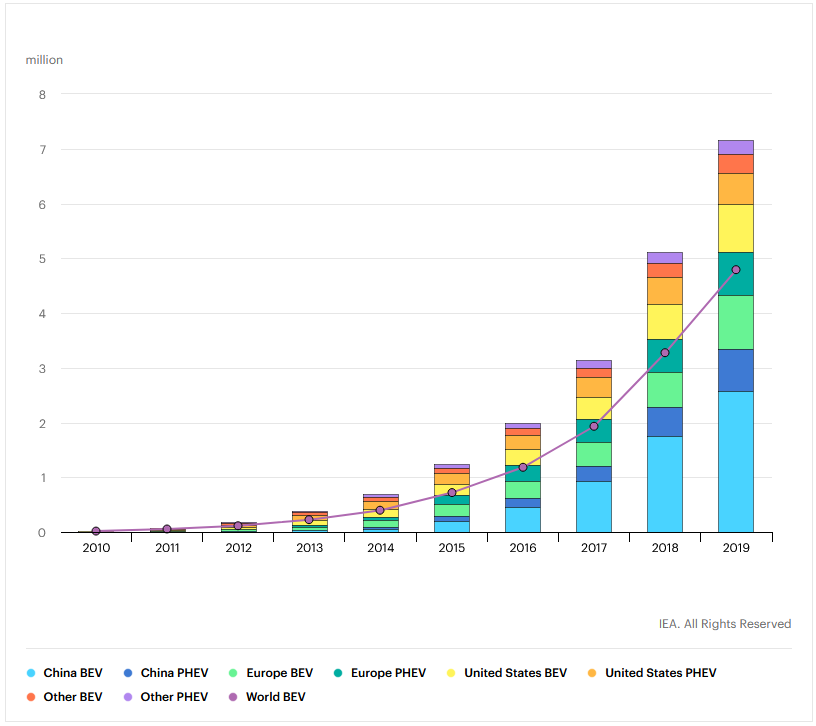
\includegraphics[width=1\linewidth]{rys01/chart.png}
        \caption{Ilość samochodów elektrycznych w różnych krajach z ciągiem czasu \cite{car_chart}}
    \label{fig:car_chart}
\end{figure}

W krajach WNP (Wspólnoty Niepodległych Państw), i być może nie tylko w nich, sporym problemem okazuje się znalezienie stacji do ładowania samochodów elektrycznych. Zdarzają się sytuacje, w których po przybyciu do stacji ładowania stacja ta okazuje się nieczynna lub położona w niedostępnym miejscu (na przykład na prywatnym terenie), a przewody umożliwiające podłączenie się są za krótkie. Dlatego nasuwa się pytanie, czy nie dałoby się jakoś poinformować właścicieli elektrycznych samochodów o tym gdzie i na jakich warunkach będą oni mogli doładować swoje pojazdy. 

Niniejsza praca jest próbą udzielenia odpowiedzi na takie pytanie. Jej temat zredagowano z myślą o stworzeniu aplikacji, która pomogłaby znaleźć działające i dostępne stacje ładowania uwzględniając bieżące położenie elektrycznego pojazdu. Ponieważ zwykle kierujący pojazdem człowiek najczęściej posługuje się telefonem (jest on znacznie poręczniejszy niż komputer, laptop czy tablet) skupiono się na aplikacji mobilnej. Biorąc pod uwagę rankingi popularności systemów na urządzenia mobilne zdecydowano, że aplikacja ta przeznaczona będzie dla urządzeń z systemem Android \cite{avi1}.


\section{Cel i zakres pracy}
Celem pracy jest zaprojektowanie i zaimplementowanie aplikacji mobilnej z połączeniem internetowym, pozwalającej ułatwiającą wyszukiwanie miejsc do ładowania samochodów elektrycznych. Aplikacja ta powinna umożliwiać gromadzenia danych o stacjach ładowania, wystawianie o nich opinii, jak również powinna pozwalać na przeglądanie zgromadzonych informacji. 

W ramach pracy powstać ma projekt aplikacji webowej, z wyróżnionymi częściami: aplikacją mobilną, usługą sieciową oraz bazą danych.
Aplikacja mobilna ma służyć do komunikacji użytkownika z usługą sieciową oraz do wizualizacji treści.
Aplikacja sieciowa zaś ma przetwarzać gromadzone informacje i zarządzać bazą danych, w której informacje te będą one składowane.

\subsection{Układ pracy}
Praca składa się z pięciu rozdziałów. W pierwszym znajduje się ogólna informacja o pracy.
W drugim skupiono się na wymaganiach dotyczących mającej powstać aplikacji oraz na wykorzystanych technologiach.
Trzeci rozdział przeznaczono na opis szczegółów implementacji poszczególnych części aplikacji.
W czwartym rozdziale opisano zagadnienie testowania stworzonej aplikacji.
% Piąty rozdział opisuję wdrożenie części serwerowej.
W ostatnim, piątym rozdziale zamieszczono podsumowanie zawierające wnioski oraz plany dalszego rozwoju aplikacji.
\chapter{Założenia projektowe}
W rozdziale opisano główny problem oraz potencjalne ścieżki prowadzące do jego rozwiązania. Zamieszczono w nim również wynik przeprowadzonej analizy wymagań funkcjonalnych i niefunkcjonalnych dla mającej powstać aplikacji. Zaproponowano ponadto makiety interfejsu użytkownika oraz przedstawiono narzędzia i technologie wybrane do realizacji celu pracy.

\section{Zarys architektury systemu}
% Описание проблемы:
% Существует проблема найти рабочую станцию зарядки, когда остается мало зарядки в автомобиле.
% Станция может не работать, плохо заряжать, может быть установлена так, что ей невозможно пользоваться, 
% различные сервисы, зачастую, ориентируются на конкретную фигрму заправок и могут не иметь самую актуальную информацию о появлении станций других производителей.
% Хочется просто взять телефон и прямо на карте увидеть где есть станции и посмотреть о ней отзывы реальных людей.

% В результате работы должно быть создано мобильное приложение в которм:
% Водители жлекторомобилей могут легко и быстро находить ближайшие зарядные станции и выбирать лучшую.
% Владельцы стнаций могут добавлять свои станции, что даст им дополнительную рекламу.
% Для определения качества станции должна использоваться система актуальных коментариев и оценок зарегестрированных пользователей.
% Каждый пользователь должен иметь собственный аккаунт для возможности пользоваться приложениемю
% Эта система позволит повысить качество зарядных пунктов.
% Это приложение полнстью поддеживается сообществом: создание и оценка станций производится пользователями.

% В пользовательском интерфейсе, которым я вляется мобильное приложение, должна быть интегрирована карта для упрощения поиска и создания мест.
% Должна быть реализована система регистарции и входа.
% Кроме пользовательского интерфейса долен быть реализована серверная часть, для обработки действий пользователей.
% А также база данных дляхранения станций и коментариев.

% Предположительный макет сервиса:
\paragraph{Opis problemu:}
Istnieje problem ze znalezieniem dobrej stacji ładującej pojazdy elektryczne.
Stacja może nie działać, źle ładować, może być zainstalowana tak, że nie można jej używać.
Większość istniejących aplikacji najczęściej ma dostęp tylko do stacji konkretnych firm i mogą nie mieć najbardziej aktualnych informacji o pojawieniu się stacji innych producentów oraz ocen rzeczywistych użytkowników.
Istnieje chęć po prostu wziąć telefon i zobaczyć bezpośrednio na mapie, gdzie są stacje i zobaczyć recenzje prawdziwych ludzi na ten temat.

\paragraph{W wyniku pracy ma powstać aplikacja mobilna w której:}
Kierowcy samochodów elektrycznych mogą łatwo i szybko znaleźć najbliższe stacje ładowania i wybrać najlepszą.
Właściciele stacji mogą dodawać swoje stacje, co da im dodatkową reklamę.
Aby określić jakość stacji, należy użyć systemu aktualnych komentarzy i ocen zarejestrowanych użytkowników.
Każdy użytkownik musi posiadać własne konto, aby móc korzystać z aplikacji.
Taki system może spowodować zwiększenie jakośi punktów ładowania pojazdów elektrycznych.
Ta aplikacja musi być w pełni wspierana przez społeczność: tworzenie i ocena stacji odbywa się przez użytkowników.

\paragraph{Przypuszczalny układ serwisu:}
Interfejs użytkownika, którym jest aplikacja mobilna, musi mieć zintegrowaną mapę, aby ułatwić wyszukiwanie i tworzenie miejsc.
Należy wdrożyć system rejestracji i logowania.
Oprócz interfejsu użytkownika musi być zaimplementowana część serwerowa do obsługi działań użytkowników.
A także baza danych do przechowywania stacji i komentarzy. Ten układ widać na rysunku \ref{fig:zarysuskladuserwisu}.
\begin{figure}[ht]
    \centering
        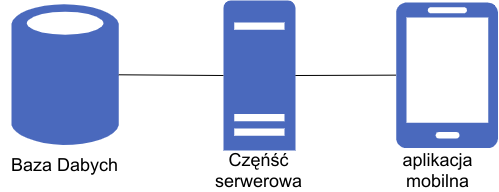
\includegraphics[width=0.4\linewidth]{rys02/uklad_wstepny.png}
        \caption{zarys uskladu serwisu \cite{diagrams_net}}
    \label{fig:zarysuskladuserwisu}
\end{figure}\newline

\section{Analiza wymagań}
\subsection{Wymagania funkcjonalne}
W tabeli \ref{tab:wymaganiafunkcjonalne} przedstawione wymagania funkc do aplikacji mobilnej razem z celem ich wdrożenia.
\begin{table}[htb] \small
    \caption{Wymagania funkcjonalne}
    \label{tab:wymaganiafunkcjonalne}
    \begin{tabular}{| m{0.5cm} | m{7cm} | m{7cm} |} 
    \hline
    № & Opis & Cel \\
    \hline
    1 & Użytkownik loguje się do własnego konta. & Umożliwia korzystanie z funkjalności aplikacji. \\ 
    \hline
    2 & Użytkownik rejestruje się. & Założenie konta tworzy nowy wpis w bazie danych pozwalający na logowanie. \\ 
    \hline
    3 & Użytkownik wyszkuję stacje ładownicze obok wybranego miejca  & dać użytkownikowi możliwość wyboru dogodnej dla niego stacji \\
    \hline
    4 & Użytkownik ma możliwość określenia własnej pozycji & Wyszukiwanie wygodniejszych stacji bardziej intuicyjne dla użytkownika  \\
    \hline
    5 & Użytkownik ma możliwość przęgliądania mapy razem ze swoją lokalizacją oraz stacji łaowniczych obok wybranego mijsca. & Ułatwienie wyszukiwania najwygodniejszej stacji ładowniczej. \\
    \hline
    6 & Użytkownik ma możliwość wyszukiwania stacji ładowniczej według słów kluczowych & Wyszukiwanie najwygoniejszej stacji z punktu widzenia typu lub nazwy stacji \\
    \hline
    7 & Użytkownik ma możliwość przeglądania informacji dotyczącej stacji ładowniczej, w tym liku oceny i komentarzy innych użytkowników & Podjęcie decyzji i dobór odpowiedniej dla użytkownika stacji ładowniczej \\
    \hline
    8 & Użytkownik ma możliwość wystawienia oceny i napisania komentarzy do wybranej stacji ładowniczej & Określenie jakości stacji. Pozwala na aktualizację danuch dotyczących stacji ladowniczej \\
    \hline
    9 & Użytkownik ma możliwość dowdawania (oznaczenia, tworzenie) nowej stacji ładowniczej & Aktualizacja informacji o dostępnych stacjach \\
    \hline
    10 & Użytkownik, który stworzył stację, ma możliwość zmiany informacji o tej stacji ładowniczej & Aktualizacja informacji istniejącej statji \\
    \hline
\end{tabular}
\end{table}

\paragraph{Diagram Przypadków użycia\newline}
Diagram przypadków użycia (rys.~\ref{fig:usecasediagram}) graficznie pokazuje użytkowników oraz funkcje aplikacji dostępne do różnych rodzajów użytkowników (w tym przypadku jeden rodzaj).
\begin{figure}[ht]
    \centering
        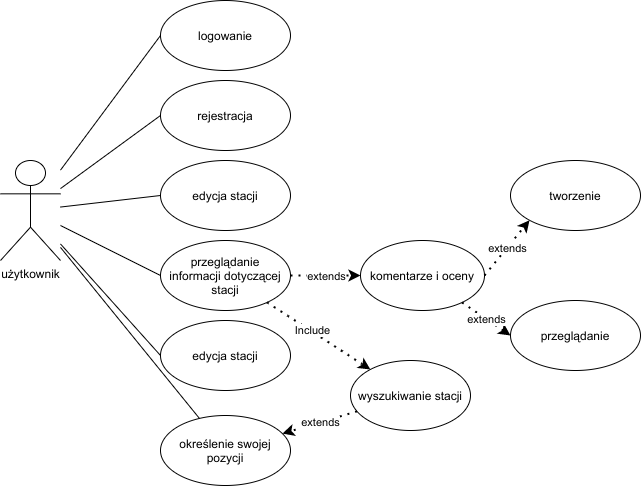
\includegraphics[width=0.7\linewidth]{rys02/use_case_diagram.png}
        \caption{dagram przypadków uzycia \cite{diagrams_net}}
    \label{fig:usecasediagram}
\end{figure}

\subsection{Wymagania niefunkcjonalne}
W tabeli \ref{tab:wymaganianiefunkcjonalne} przdstawione wymagania niefunkcjonalne: krótki opis wymagania, typ (jakiej dziedziny to dotyczy) oraz uwagi do tego wymagania.
\begin{table}[htb] \small
    \caption{Wymagania niefunkcjonalne}
    \label{tab:wymaganianiefunkcjonalne}
    \begin{tabular}{| m{0.5cm} | m{3cm} | m{5.75cm} | m{5.75cm} |} 
    \hline
    № & typ & Opis & Uwagi \\
    \hline
    1 & Bezpiczeństwo & Hasła muszą być przechowywane w biezpicznej formie & Hasła nie przchowyją się w pierwotnej formie, tylko w formie zaszyfrowanej \\ 
    \hline
    2 & Bezpiczeństwo & Małe ryzyka przechwytywania hasła przez trzecich osób podczas komunikacji interfejsu użytkownika i części serwerowej & Autentykacja użytkownika na serwerze powinna zachodzić za pomocą tokenów \\ 
    \hline
    3 & Przenoszlność & wdrożenie systemu powinno być szybkie i łatwe & \\ 
    \hline
    4 & Konfigurowalność & Zmiana ustaleń bez konieczosści rekompilacji części serwerowej & Zarządzaniem portu na którym działa część serwerowa, wymiana adresu oraz nazwy kolekcji bazy danuch, musi być możliwa za pomocą pliku konfiguracyjnego \\ 
    \hline
    5 & Estetyczne & Przyjazny interfajs użytkownika & Intuicyjny i zrozumiały interfejs \\ 
    \hline
    6 & Ergonomia & Interfejs w języku angielskim & Możliwość kożystania z aplikacji przez dużą libzi \\
    \hline
    7 & Przenoszlność & Aplikacja mobilna musi działać na 90\% lub więcej telefonów pracujących na systemie Android & Możliwość kożystania z aplikacji przez dużą ilość ludzi \\
    \hline
    8 & Estetyczne & kolory muszą być odpowiednio dopasowane & Wykorzystanie małej dopasowanych do sobie ilośći kolorów  \\
    \hline
    9 & Wydajność & Srzybka reakcja systemu & System musi szybko reagować na działania użytkownika \\
    \hline
    10 & Informatywność & System powinien powiadomiać o błędach i sukcesach  & Podczas rażądzania systemem użytkownik powinin zawze wiedzieć jaki wynik jego działania \\
    \hline
    11 & Ergonomia & Wykorzystanie z aplikacji mobilnej za pomocą jednej ręki & Przyciski muszą znajdować się w dolnej części ekranu lub znajdować się w dostępnym miejscu \\
    \hline
    12 & Estetyczne & Wszystkie elementy muszą być w jednym stylu & Niedopuszczalne jest użycie różnych czcionek oraz ciągłej zmiany kolorów \\
    \hline
    13 & Dostęp & Część serwerowa zrobiona zgodnie z regułami Rest (ang. \textit{Representational State Transfer}) API (ang. \textit{Application Programming Interface}) & Przestrzeganie się Best Prakties Rest API \cite{rest_api_best}] \\
    \hline
    14 & Ergonomia & Dla realizacji mapy wykorzystuję się Google Maps[index] & Ułatwia rozumienie interfejsu dla użytkowników \\
    \hline
\end{tabular}
\end{table}
\newpage
\subsection{Nażędzia i technologie}
Do sworzenia aplikacji mobilnej, części serwerowej oraz bazy daych zostały wybrane następujące narzędzia i technologie:
\begin{multicols}{3}
\begin{itemize}
    \item Visual Studio Code;
    \item Go;
    \item REST API;
    \item JWT;
    \item MongoDB;
    \item Redis;
    \item Android Studio;
    \item Gradle;
    \item Android SDK;
    \item Java JDK 8;
    \item RxJava 2;
    \item Google Cloud Platform;
    \item GMS;
    \item Docker;
\end{itemize}
\end{multicols}
\paragraph{Visual Studio Code} \cite{vscode} to darmowy edytor kodu źródłowego, który został wyprodukowany przez Microsoft. Działa na systemach Windows, Linux, macOS. Jest rozszerzalny za pomocą plug-inów.
Lista podtrzymywanych języków i możliwości jest dość wielka i może być rozszerzona za pomocą plug-inów. Kilka funkcji: podświetlanie składni, IntelliSense, refaktoryzacja, debugowanie i inne.

\paragraph{Go} (golang) \cite{golang1,golang2,golang3,godoc} jest językiem programowania. Kompilowany, wielowątkowy. Stworzony przez Google. Kod tego języku może być kompilowany do Linux, Windows, macOS, FreeBSD, Android i inne.
Język jest przeznaczony do budowania serwisów z wysokim obciążeniem i efektywnością, które pracują na systemach rozproszonych z wielowątkowymi procesorami.

\paragraph{REST API} (ang. \textit{REpresentational State Transfer}) (ang. \textit{Application Programming Interface}) \cite{rest_api,rest_api_best} Jest to popularne podejście w architekturze tworzenia interfejsów programistycznych.
Podstawowe zasady to: architektura klient-serwer (na przykład przydzielamy klienta i magazyn danych), brak stanu (serwer nie przechowuje stanu klienta, wszystkie potrzebne informacje są wysyłane wraz z żądaniem),
buforowalność (buforowanie danych jest dozwolone, jeśli w odpowiedzi jest na to zgoda), jednorodność interfejsu (ograniczenia stylu pisania), wielopoziomowość systemu (komponenty systemu mają bezpośredni dostęp tylko do sąsiednich warstw), łatwość rozszerzenia funkcjonalności (opcjonalnie).

\paragraph{JWT} (ang. \textit{JSON Web Token}) \cite{jwt} jest standardem, który jest przeznaczony do tworzenia tokenów dostępu. Za pomocą JWT sprawdza się, czy wchodzące dane zostały wysłane przez autoryzowane źródło.
Składa się z trzech części: nagłówek (informacja o tym, w jaki sposób odszyfrować token), dane (zaszyfrowane dane) oraz sygnatura. Każdy taki token ma czas działania. Nie może być oznaczony jako nieroboczy, dopóki nie skończy się czas jego działania.

\paragraph{MongoDB} \cite{mongoDB,mongoDB_doc,mongodb_habr} jest NoSQL (ang. \textit{Not only Structured Query Language}) rozwiązaniem do przechowywania danych. Dane przehowywane w formacie BSON (ang. \textit{Binary JavaScript Object Notation}).
Format licencji SSPL (ang. \textit{Server Side Public License}). Wykorzystuje technikę segmentacji obiektów bazy danych, co pozwala na bilansowanie obciążenia.

\paragraph{Redis} \cite{redis} system zarządzania bazami danych klasy NoSQL, który współpracuje ze strukturami danych typu ,,klucz-wartość''. Najczęściej używa sie do implementacji baz dabych, pamięci podręcznej, brokerów wiadowmości.

\paragraph{Android Studio} \cite{android_doc,android_studio} zintegrowane środowisko programistyczne, które zostało wyprodukowane przez JetBrains na podstawie IelliJ IDEA, do budowania aplikacji na platformie Android. Jest dostępna do systemów Windows, Linux, macOS. Jest udostępniona za pomocą bezpłatnej licencji Apache 2.0.

\paragraph{Gradle} \cite{gradle,gradle_android_doc} jest systemem automatycznego budowania aplikacji oraz zarządzania zależnościami, który służy do uproszczenia pracy z językiem Java.

\paragraph{Android SDK} \cite{android_studio} (ang. \textit{Software development kit}) jest narzędziem do tworzenia aplikacji mobilnych dla systemów na bazie Android, które został wyprodukowane przez Google.
Ten zestaw SKD zawiera nażędzia programistyczne: zestaw bibliotek Android i Java, emulator telefonu, debugger, dokunentację, szablony prostych aplikacji.

\paragraph{Java JDK 8} (and. \textit{Java Development Kit}) \cite{java_doc} jest zestawem programisty do programowania w języku Java. Zawiera: kompilator języka Java, przykłady, dokumentację, system uruchomiania koda Java (JDK (ang. \textit{Java Runtime Environment})).
Java jest językiem ogólnego zastosowania, obiektowym, krosplatformowym, dzięki uruchomianiu się kodu na maszynie wirtualnej. Został wyprodukowany przez Sun Microsystems.
Przy tworzeniu aplikacji został użyty język wersji 8, ponieważ kompatybilność tej wersji jest bardzo wysoka.

\paragraph{RxJava 2} jest to biblioteka pozwalająca na stosowanie reaktywnego programowania w języku Java. Programowanie reaktywne jest paradygmatem programowania pozwalającym na programowanie z asynchronicznymi strumieniami (sekwencja stałych zderzeń, które posortowane według czasu) danych.
Ta biblioteka jest bardzo przydatna na przykład, żeby interfejs użytkownika ciągle był dostępny do użycia, nawet w podczas obliczania jakiejś logiki, na przykład oczekiwanie odpowiedzi od serwera.

\paragraph{Google Cloud} \cite{google_cloud} jest pakietem Google usług w chmurze. Ten serwis pozwala na wykorzystanie serwisów Google Search, Gmail, przechowywanie plików, Youtube, obliczenie i przechowywanie danych, uczenie maszynowe i inne usługi, z których korzysta Google w swoich projektach.
Usługa ta jest płatna. Różne części mają różne koszty w zależności od ilości zapytań do serwisów Google. Jeśli koszty użycia tych serwisów mniej niż 200 dolarów miesięcznie, Google nie pobiera opłaty. W tej pracy inżynierskiej został wykorzystany serwis Static Maps \cite{google_cloud_pricing}.
Ten serwis jest darmowy przy tworzeniu oprogramowania do telefonów (Android Maps SDK for Android (ang. \textit{Maps Software development kit for Android}) \cite{maps_sdk}).

\paragraph{GMS}  (and. \textit{Google Mobile Services}) jest to zestaw aplikacji dostarczonych przez Google: Goole Maps, Google Paly Store, Gmail Google Drive Google Duo, Google Chrome, Google Photos, Google TV, YOutube, Youtube Music.

\paragraph{Docker} \cite{docker,docker_doc} jest to oprogramowanie przeznaczone do automatyzacji wdrażania i zarządzania aplikacjami. Aplikacje uruchamiają się w kontenerach. Docker pozwala na upakowanie aplikacji oraz wszystkich zależności w niezależny od podstawowego systemu kontener, który może być łatwo przeniesiony na dowolny *nix system.

% Jako Baza danych wykorzystuje się NoSQL (ang. (ang. \textit{Not only Structured Query Language}) baza danych MongoDB \cite{mongoDB,mongoDB_doc}.
% Część serwerowa napisana w języku Go \cite{golang1,golang2,golang3,godoc} w architekturze Rest API \cite{rest_api_best}.
% Część serwerowa i Baza Danych muszą uruchamiać się w Docker kontenerze \cite{docker,docker_doc}.
% Aplikacja mobilna działa w systemie Android za pomocą Android Studio \cite{android_doc,android_studio,gradle,gradle_android_doc} w języku Java \cite{java_doc}.
% Dla realizacji Google Maps w aplikacji mobilnej wykorzystuję się serwis Google Cloud \cite{google_cloud} Maps SDK for Android (ang. \textit{Maps Software development kit for Android}) \cite{maps_sdk}.
% 
\subsection{Makiety interfejsu użytkownika}
Po analizie wymagań zostały stworzone możliwe makiety aplikacji, która ma powstać.

Na dole ekranu aplikacji znajduje się główne menu zawierające 4 pozycje: mapę, wyszukiwanie stacji, tworzenie stacji i parametry.
Na rysunku \ref{fig:search_makiet}a przedstawiono pierwszy etap wyszukiwania stacji ładowania.
Pod polem wyszukiwania znajduje się rozwijane menu, które pozwala wybierać typ wyszukiwania, w tym wyszukiwanie na podstawie pozycji użytkownika oraz nazwy i opisu stacji.
Poniżej znajduje się możliwość do zmiany dystansu wyszukiwania oraz przycisk wyszukiwania.
\begin{figure}[ht]
	\centering
  \begin{tabular}{@{}rl@{\hspace{10mm}}rl@{}}
  a) & \vtop{\vskip-2ex\hbox{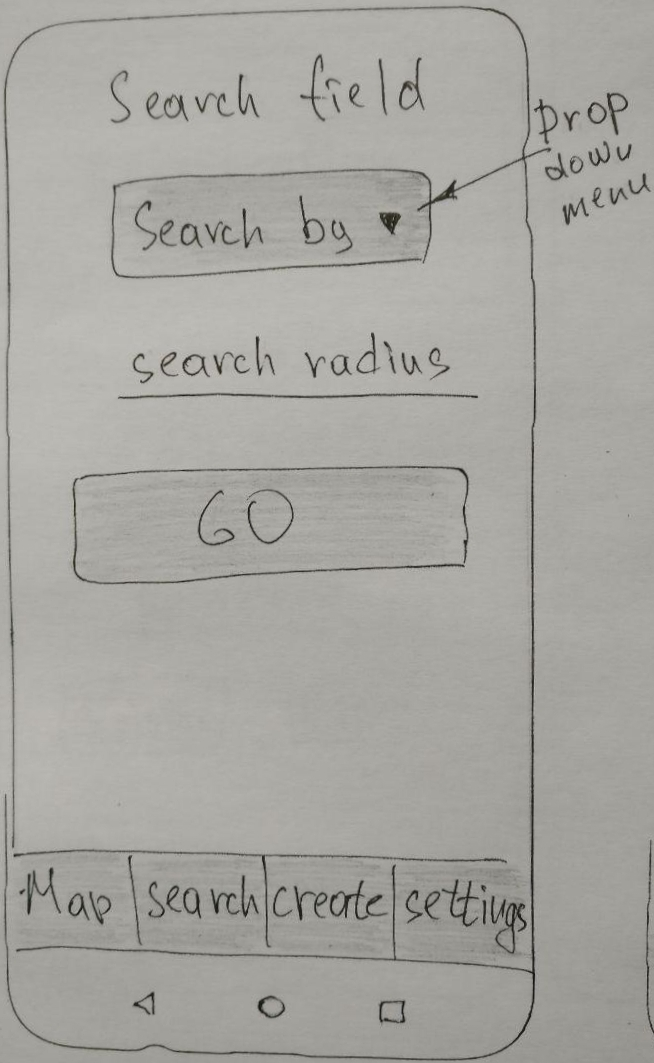
\includegraphics[width=0.30\linewidth]{rys02/search_makiet.jpg}}} &
	b) & \vtop{\vskip-2ex\hbox{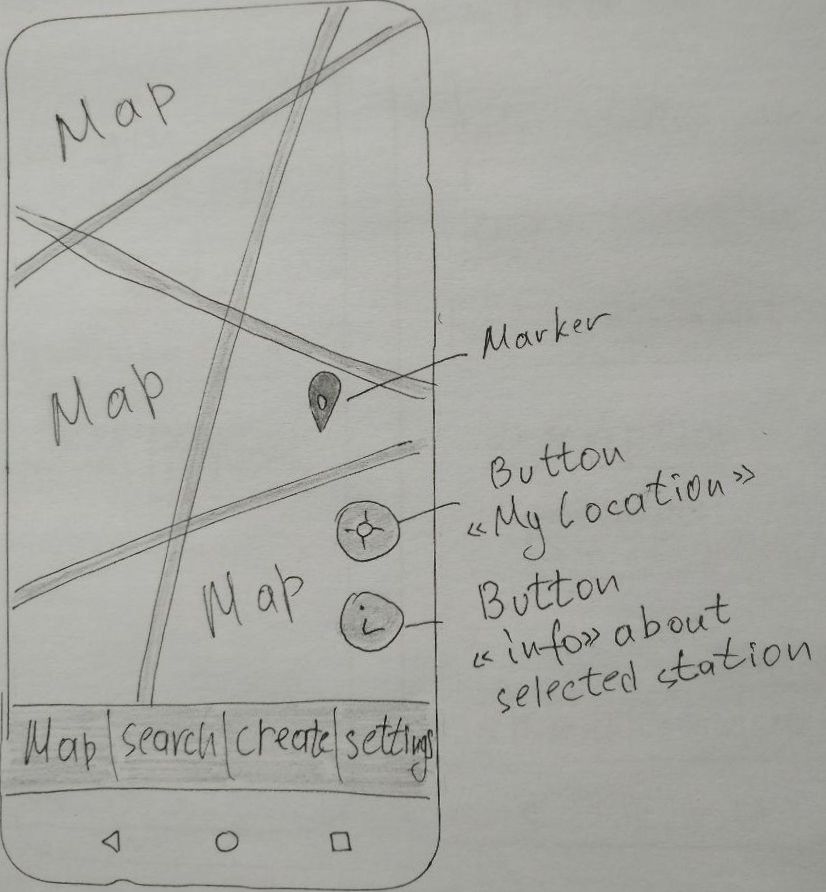
\includegraphics[width=0.45\linewidth]{rys02/main_makiet.jpg}}} 
		\end{tabular}
        \caption{Makiety interfejsów aplikacji mobilnej: a) strona wyszukiwania stacji ładowania, b) strona główna.}
    \label{fig:search_makiet}
\end{figure}

Na rysunku~\ref{fig:search_makiet}b przedstawiono makietę pozwalającą dokonać wyboru stacji ładowania. Stacje poznaczone znacznikami na mapie. Dla otrzymania informacji o wybranej stacji (wybierany jest markier na mapie) oraz wyświetlania pozycji użytkownika wykorzystują się okrągłe przyciski z lewej strony ekranu.

Podczas tworzenia stacji ładowania (rys. \ref{fig:create_makiet}) dla wygody użytkowania można wybrać miejsce na mapie poprzez odpowiedni przycisk.
\begin{figure}[ht]
    \centering
        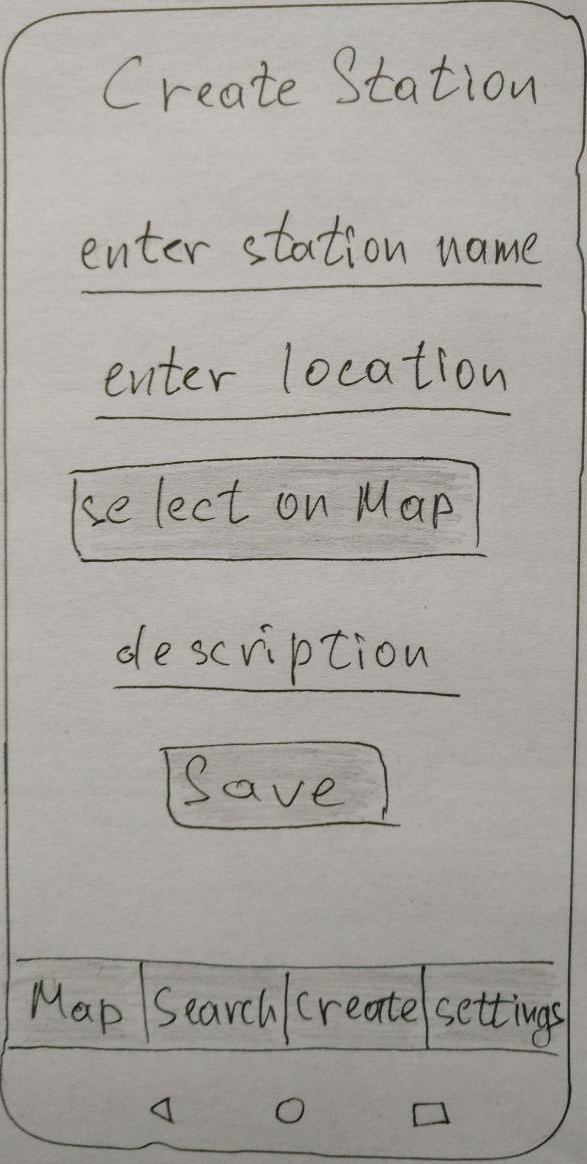
\includegraphics[width=0.3\linewidth]{rys02/create_makiet.jpg}
        \caption{makiet strony tworzenia stacji ładowania}
    \label{fig:create_makiet}
\end{figure}
\newpage
Na stronie informacji o stacji (rys.\ref{fig:station_makiet}) oprócz nazwy stacji, opisu oraz oceny, wyliczonej na podstawie komentarzy oceny, znajdują się komentarzy uzytkowników w porządku: najpierw najnowsze.
% TO DO: proszę ułożyć dwie makiety obok siebie, jak w przykładzie powyżej
\begin{figure}[ht]
    \centering
        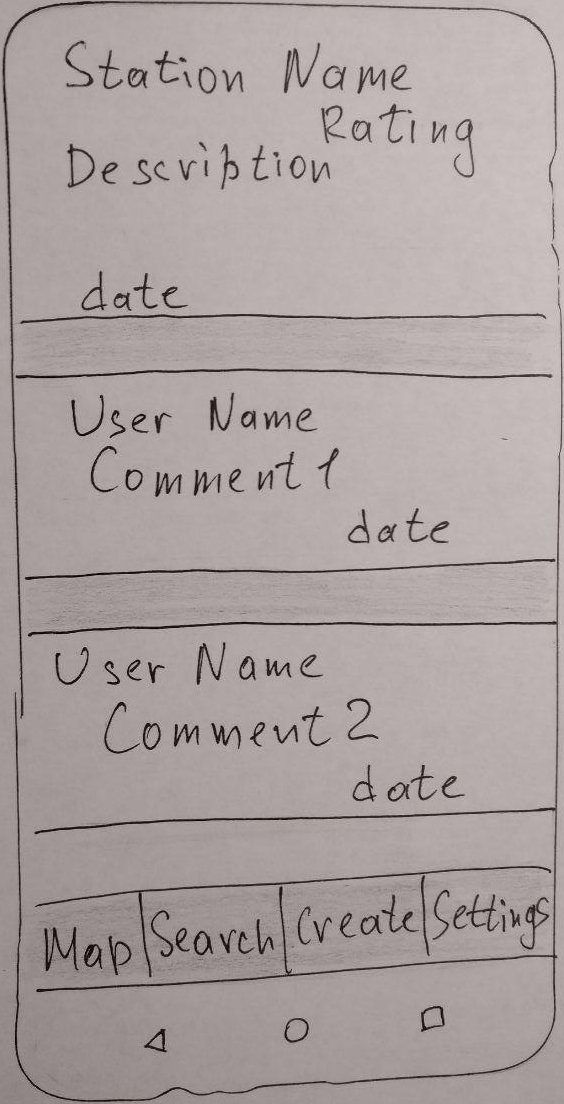
\includegraphics[width=0.3\linewidth]{rys02/station_makiet.jpg}
        \caption{makiet strony informacji o stacji ładowania}
    \label{fig:station_makiet}
\end{figure}
\newline
Dla rejestracji i logowania wykorzystują się dwa różne ekrany (rys.\ref{fig:login_makiet} oraz \ref{fig:register_makiet})
\begin{figure}[ht]
    \centering
        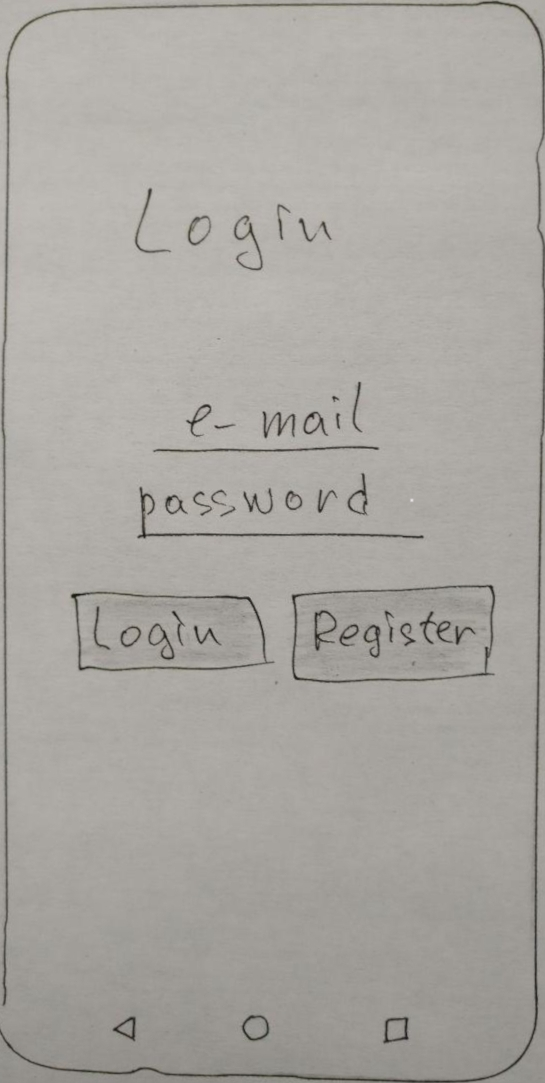
\includegraphics[width=0.3\linewidth]{rys02/login_makiet.jpg}
        \caption{makiet strony logowania}
    \label{fig:login_makiet}
\end{figure}
\begin{figure}[ht]
    \centering
        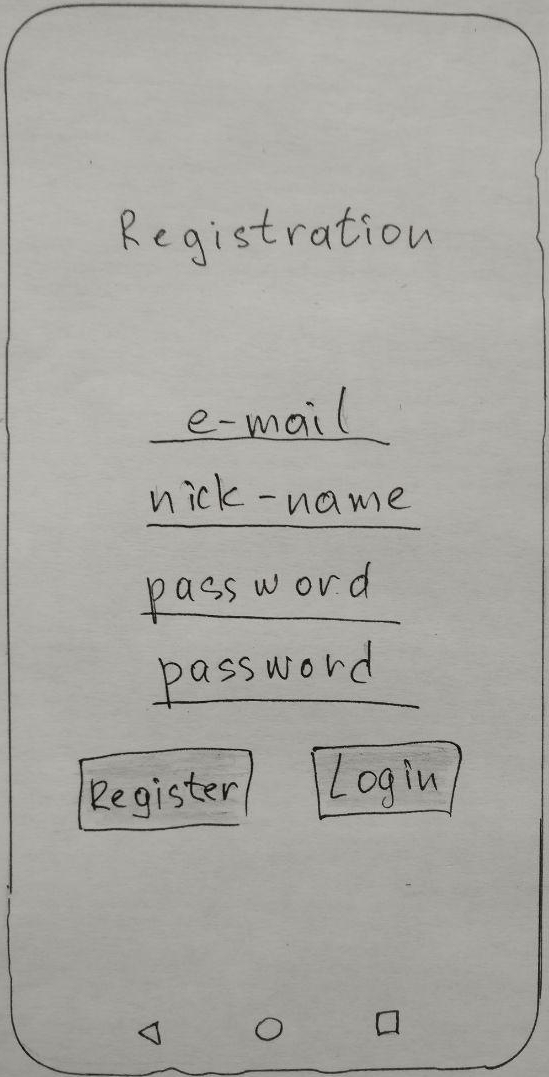
\includegraphics[width=0.3\linewidth]{rys02/register_makiet.jpg}
        \caption{makiet strony rejestracji}
    \label{fig:register_makiet}
\end{figure}
\newpage



% \paragraph{Część serwerowa:}
% \begin{itemize}
%     \item Visual Studio Code
%     \item Go
%     \item MongoDB
%     \item Redis
%     \item Docker ?
%     \item Docker-compose ?
%     \item Go Modules
%     \item gorilla/mux
%     \item sirupsen/logrus
%     \item mongo-driver
%     \item go-redis/redis
%     \item go-ozzo/ozzo-validation
%     \item yaml.v2
%     \item google/uuid
% \end{itemize}

% \paragraph{Aplikacja mobilna:}
% \begin{itemize}
%     \item Android Studio
%     \item Java   
%     \item ? gradle ?
%     \item RxJava
%     \item OkHttp 3
%     \item Retrofit 2
%     \item Maps SDK for Android
%     \item Google Play services APIs
%     \item gson
% \end{itemize}

% \paragraph{Testowanie: ??}
% \begin{itemize}
%     \item Postman
%     \item MongoDB Compass
%     \item stretchr/testify ??
% \end{itemize}


% \paragraph{Paragraf}
% Tekst\newline
% Tekst

\chapter{Implementacja aplikacji}
%
\section{Model bazy danych}
W systemie wykorzystano dwie nierelacyjne bazy danych: MongoDB i Redis.
MongoDB jest przeznaczona do przechowywania danych aplikacji.
Redis wykorzystuje się tylko do czasowego przechowywania tokenów.

% 
\paragraph{MongoDB\newline}
% TO DO: proszę stosować czcionkę maszynową do kodu źródłowego, nazw zmiennych i klas, nazw plików itp.
% DONE: dziękuję, po prostu nie wiedziałem jak to zrobić z nazwami.
% TO DO: aby zdefiniować zawartość plików json można posłużyć się specyfikacją json schema : https://json-schema.org/
% TO DO: prawdopodobnie dokumenty w MongoDB powstają poprzez mapowanie z obiektów dostępnych w języku programowania,
%  jeśli tak jest, to należy o tym powiedzieć (w opisie implementacji można pokazać diagram klas zawierających odpowiednie pola)
% TO VERIFY: ten json jest wycinkiem z konsoli bazy danych ,,mongo'' po wprowadzeniu odpowiedniego zapytania (,,db.nazwakolekcji.find({});''), różni się od odpowiedzi, które otrzymałem w tej konsoli tym, że sformatowano do czytelnego tekstu, a nie wszystko w jednej linii.
Baza danych składa się z dwóch kolekcji: \texttt{station} i \texttt{user}. Kolekcja \texttt{user} składa się z następujących pól:
\texttt{
    \begin{itemize}
        \item \_id : ObjectId(String)
        \item user\_name : String
        \item email : String
        \item password : String
        \item Model : Object :
        \begin{itemize}
            \item create\_at : ISODate
            \item update\_at : ISODate
            \item delete\_at : ISODate
        \end{itemize}
    \end{itemize}
}

Przykład encji:
\begin{lstlisting}[basicstyle=\tiny\ttfamily]
    {
        "_id":ObjectId("5fb93e4b721953b7c60983c6"),
        "user_name":"newtest",
        "email":"newtest@test.test",
        "password":"$2a$04$o0WfZvdk4WUpsct.BH3zw.3MFJFmUuLe8VjJx2OeyxtZuBliMOrl.",
        "model":{
            "create_at":ISODate("2020-11-21T16:20:27.044Z"),
            "update_at":ISODate("2020-11-21T16:20:27.044Z"),
            "delete_at":ISODate("0001-00-00T00:00:00Z")
        }
    }
\end{lstlisting}

Kolekcja \texttt{station} składa się z następujących pól:
\texttt{
    \begin{itemize}
        \item \_id : String
        \item station\_name : String
        \item owner\_id : String
        \item rating : Double
        \item latitude : Double
        \item longitude : Double
        \item description : String
        \item comments : Array :
        \begin{itemize}
            \item \_id : String
            \item user\_id : String
            \item user\_name : String
            \item text : String
            \item rating : Double
            \item model : Object :
            \begin{itemize}
                \item create\_at : ISODate
                \item update\_at : ISODate
                \item delete\_at : ISODate
            \end{itemize}
        \end{itemize}
        \item model : Object :
        \begin{itemize}
            \item create\_at : ISODate
            \item update\_at : ISODate
            \item delete\_at : ISODate
        \end{itemize}
    \end{itemize}
}

Przykład encji:
\begin{lstlisting}[basicstyle=\tiny\ttfamily]
    {
        "_id":ObjectId("5fca6f81bb37f04ad438c1a5"),
        "station_name":"Station Name",
        "owner_id":"5fb828babe10c57ba70d49cd",
        "rating":3.6666666666666665,
        "description":"description",
        "latitude":57.12662933894774,
        "longitude":14.208925142884254,
        "model":{
            "create_at":ISODate("2020-12-04T17:18:57Z"),
            "update_at":ISODate("2020-12-04T17:20:55Z"),
            "delete_at":ISODate("0001-00-00T00:00:00Z")
        },
        "comments":[
            {
                "_id":"5fca6ff7bb37f04ad438c1a8",
                "user_id":"5fb828babe10c57ba70d49cd",
                "user_name":"test",
                "text":"  Comment 3",
                "rating":5,
                "model":{
                    "create_at":ISODate("2020-12-04T17:20:55Z"),
                    "update_at":ISODate("2020-12-04T17:20:55Z"),
                    "delete_at":ISODate("0001-00-00T00:00:00Z")
                }
            },
            {
                "_id":"5fca6fe5bb37f04ad438c1a7",
                "user_id":"5fb828babe10c57ba70d49cd",
                "user_name":"test",
                "text":" Comment 2",
                "rating":3,
                "model":{
                    "create_at":ISODate("2020-12-04T17:20:37Z"),
                    "update_at":ISODate("2020-12-04T17:20:37Z"),
                    "delete_at":ISODate("0001-00-00T00:00:00Z")
                }
            },
            {
                "_id":"5fca6fb8bb37f04ad438c1a6",
                "user_id":"5fb828babe10c57ba70d49cd",
                "user_name":"test",
                "text":"Comment 1",
                "rating":3,
                "model":{
                    "create_at":ISODate("2020-12-04T17:19:52Z"),
                    "update_at":ISODate("2020-12-04T17:19:52Z"),
                    "delete_at":ISODate("0001-00-00T00:00:00Z")
                }
            }
        ]
    }
\end{lstlisting}

% 
\paragraph{Redis\newline}
Baza danych Redis wykorzystana tylko dla przechowywania tokenów użytkowników, które już wylogowane, ponieważ jedną z wad JWT tokenów jest to, że wygenerowany token nie można zrobić nieważny, dopóki nie skończy się czas jego działania.
Redis częściowo eliminuje ten problem.

W nim przechowuje się para klucz - wartość, pewny czas. Po upływie tego czasu zapis automatycznie jest usuwany.
Dla szybkiego wyszukiwania encja wygląda w następujący sposób: \texttt{token}, \texttt{token}. To pozwala często wylogować użytkowniku, ale zajmuje więcej miejsca niż encja typu: \texttt{user\_id}, \texttt{token}.

\section{Implementacja części serwerowej}
% 
\subsection{Struktura RestApi}
% 
\subsubsection{Narzędzia, technologie, biblioteki}
Do stworzenia serwerowej części aplikacji użyto następujących technologii:
\begin{itemize}
\item Visual Studio Code - środowisko programistyczne;
\item Go - język programowania;
\item Go Modules - system zarządzania zależnościami;
\item gorilla/mux - Router mapuje przychodzące żądania na listę zarejestrowanych tras i wywołuje moduł obsługi tego żądania, który odpowiada URL (ang. \textit{Uniform Resource Locator}) adresowi;
\item sirupsen/logrus - rejestrator strukturalny;
\item mongo-driver - sterowanie MongoDB z języka Go;
\item go-redis/redis - sterowanie Redis z języka Go;
\item dgrijalva/jwt-go - realizacja JWT w języku Go;
\item crypto/bcrypt - realizuje algorytm haszowania bcrypt Provosa i Mazierao;
\item go-ozzo/ozzo-validation - pakiet wspomagający na walidację danych;
\item yaml.v2 - implementuje obsługę YAML (ang. \textit{Yet Another Markup Language});
\item google/uuid - sprawdza i generuje UUID (ang. \textit{universally unique identifier});
\end{itemize}

% 
\subsubsection{Struktura plików RestApi}
Na rysunku \ref{fig:backend_file_structure} została przedstawiona struktura plików części serwerowej. Obok plików, niezbędnych do działania aplikacji, znajdują się pliki pozwalające na prowadzenie testów jednostkowych. Te pliki mają nazwę w postaci \texttt{*\_test.go}.
% TO DO: proszę poukładać obrazki ze strukturami plików obok siebie (pojedynczo zajmują za dużo miejsca)
% TO VERIFY:
\begin{figure}[ht]
\centering
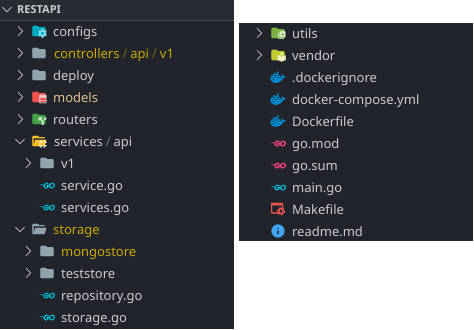
\includegraphics[width=0.25\linewidth]{rys03/backend_file_structure.png}
\caption{Struktura plików}
\label{fig:backend_file_structure}
\end{figure}
\begin{figure}[ht]
	\centering
    \begin{tabular}{@{}rl@{\hspace{3mm}}rl@{\hspace{3mm}}rl@{}}
        a) & \vtop{\vskip-2ex\hbox{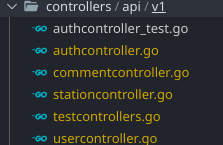
\includegraphics[width=0.25\linewidth]{rys03/controllers.png}}} &
        b) & \vtop{\vskip-2ex\hbox{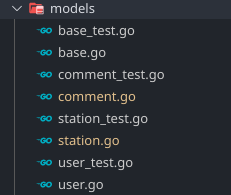
\includegraphics[width=0.25\linewidth]{rys03/model.png}}} &
        c) & \vtop{\vskip-2ex\hbox{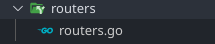
\includegraphics[width=0.25\linewidth]{rys03/routers.png}}}
    \end{tabular}
    \caption{Struktura plików: a) kontrolery, b) modeli danych, c) routery.}
    \label{fig:backend_file_structure_1}
\end{figure}
\begin{figure}[ht]
	\centering
    \begin{tabular}{@{}rl@{\hspace{3mm}}rl@{\hspace{3mm}}rl@{}}
        a) & \vtop{\vskip-2ex\hbox{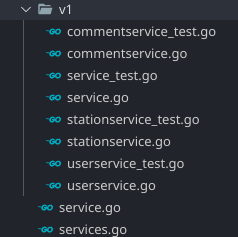
\includegraphics[width=0.25\linewidth]{rys03/services.png}}} &
        b) & \vtop{\vskip-2ex\hbox{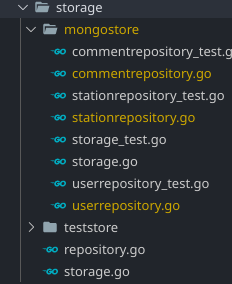
\includegraphics[width=0.25\linewidth]{rys03/storage.png}}} &
        c) & \vtop{\vskip-2ex\hbox{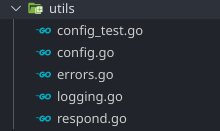
\includegraphics[width=0.25\linewidth]{rys03/utils.png}}}
    \end{tabular}
    \caption{Struktura plików: a) serwisy, b) wszpółdziałania z bazą danych, c) narzędzia.}
    \label{fig:backend_file_structure_2}
\end{figure}

Katalog \texttt{config} zawiera pliki konfiguracyjne. W katalogu \texttt{controllers} (rys.~\ref{fig:backend_file_structure_1}a) znajdują się kontrolery, które są wykorzystywanie do połączenia poziomu serwisów z punktami końcowymi serwera (ang.~\emph{endpoints}).

Do katalogu \texttt{deploy} jest kompilowana aplikacja przy uruchomieniu \texttt{Makefile}.

Katalog \texttt{models}(rys. \ref{fig:backend_file_structure_1}b) zawiera modeli danych do przechowywania w bazie danych oraz do przekazania do interfejsu użytkownika.

Katalog \texttt{routers} (rys. \ref{fig:backend_file_structure_1}c) zawiera plik, w którym zachodzi mapowanie punktów końcowych z kontrolerami.

Funkcje lub metody przechowywane w katalogu \texttt{services} (rys. \ref{fig:backend_file_structure_2}a) prowadzą obróbkę danych i podejmują decyzję co z nimi trzeba zrobić.

Współpraca z bazą danych zachdzi w katalogu \texttt{storage} (rys. \ref{fig:backend_file_structure_2}b). Katalog \texttt{mongostore} wspódziałuje z MongoDB, notomiast \texttt{teststore} wykorzystuje się do testowania, które będzie omówione w odpowiednim rozdiale \ref{ch:Testy}.

W katalogu \texttt{utils} (rys. \ref{fig:backend_file_structure_2}c) znajdują się rzeczy wspomagające, naprykład lista błedów lub rejestracja działania serwera.


\subsubsection{KOnfiguracja serwera}
Do zapobiegania ponowniej kompilacji w przypadku zmiany portu, na którym działa serwer lub adresów baz danych, została utworzona struktura \texttt{Config} \ref{list:config_restapi} (plikutils/config.go), która przy uruchomienui aplikacji pobiera dane z pliku, który zostanie podany jako parametr wejściowy.
Plik musi być typu \texttt{yaml}. Za pomocą biblioteki \texttt{yaml.v2} ten plik jest parsowany do obiektu struktury \texttt{Config} \ref{list:config_restapi_new}. Przykład pliku:
\begin{lstlisting}[basicstyle=\tiny\ttfamily]
    bind_addr: :8081
    database_url: mongodb://127.0.0.1:27017
    db_name: elCharge
    db_user_collection: user
    db_station_collection: station
    db_redis: 127.0.0.1:6379
    jwtKey: 21d5680b6a
\end{lstlisting}

\begin{lstlisting}[label=list:config_restapi,caption=Klasa konfiguracyjna części serwerowej,basicstyle=\tiny\ttfamily]
    type Config struct {
        BindAddr            string `yaml:"bind_addr"`
        DatabaseURL         string `yaml:"database_url"`
        DbName              string `yaml:"db_name"`
        DbUserCollection    string `yaml:"db_user_collection"`
        DbStationCollection string `yaml:"db_station_collection"`
        RedisDB             string `yaml:"db_redis"`
        JWTKey              string `yaml:"jwtKey"`
    }
\end{lstlisting}

\begin{lstlisting}[label=list:config_restapi_new,caption=Wczytanie pliku konfiguracyjnego części serwerowej,basicstyle=\tiny\ttfamily]
    func NewConfig(path string) (*Config, error) {
        configFile, err := ioutil.ReadFile(path)
        if err != nil {
            return nil, err
        }
        config := &Config{}
        err = yaml.Unmarshal(configFile, config)
        if err != nil {
            return nil, err
        }
        return config, nil
    }
\end{lstlisting}
% 
\subsubsection{Przepływ danych}
Na rysunku \ref{fig:backend_data_flow} został przedstawiony schemat przetwarzania i przepływu danych przy wysyłaniu zapytania do części serwerowej niniejszej aplikacji.
% TO DO: rysunek do przerysowania (proszę zacieśnić bloczki, wtedy przy skalowaniu do szerokości strony czcionka stanie się większa
% DONE:
\begin{figure}[ht]
\centering
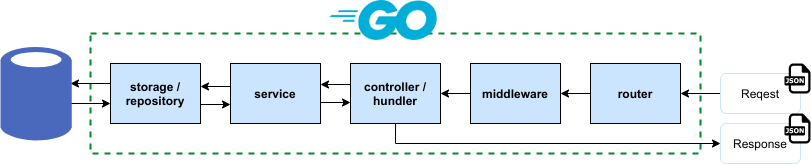
\includegraphics[width=1\linewidth]{rys03/backend_data_flow.png}
\caption{Przepływ danych}
\label{fig:backend_data_flow}
\end{figure}

% 
\subsubsection{Punkty końcowe}
Część serwerowa jest napisana zgodnie z modelem Rest API. Wymiana danymi zachodzi za pomocą standardów: HTTP (ang. \textit{HyperText Transfer Protocol}), URL, JSON.
W tabeli \ref{tab:endpoints} przedstawiony spis endpointów razem z metodą ich wysłania oraz krótkim opisem.
\begin{table}[htb] \small
    \caption{Lista Enpointów części serwerowej}
    \label{tab:endpoints}
    \begin{tabularx}{\linewidth}{| m{0.45cm} | m{1.5cm} | m{6cm} | X |}
    \hline
    № & Metoda & Endpoint & Opis \\
    \hline
    1 & GET & /api/v1 & Endpoint do testowania działania serwera. \\
    \hline
    2 & POST & /api/v1/login & Zalogowanie się użytkownika. \\
    \hline
    3 & GET & /api/v1/logout & Wylogowanie się użytkownika. \\
    \hline
    4 & POST & /api/v1/users & Tworzenie użytkownika / rejestracja \\
    \hline
    5 & GET & /api/v1/users/{id} & Wczytywanie danych jednego użytkownika. \\
    \hline
    6 & PUT & /api/v1/users/{id} & Edycja użytkownika. \\
    \hline
    7 & DELETE & /api/v1/users/{id} & Usuwanie użytkownika. \\
    \hline
    8 & GET & /api/v1/users/read?skip=""\&limit="" & Wczytywanie danych limitowanej listy użytkowników użytkownika. \\
    \hline
    9 & POST & /api/v1/stations & Tworzenie stacji ładowniczej. \\
    \hline
    10 & GET & /api/v1/stations/{id} & Wczytywanie danych jednej stacji ładowniczej. \\
    \hline
    11 & PUT & /api/v1/stations/{id}?ownid="" & Edycja stacji. \\
    \hline
    12 & DELETE & /api/v1/stations/{id} & Usuwanie stacji ładowniczej. \\
    \hline
    13 & GET & /api/v1/stations/read?skip=""\&limit=""\&lat=""\&lng=""\&dist=""\&descr=""\&nam="" & Wyszukiwnaie stacji ładowniczej w zależności od parametrów. \\
    \hline
    14 & POST & /api/v1/stations/{sid}/comments & Tworzenie komentarza. \\
    \hline
    15 & GET & /api/v1/stations/{sid}/comments{id} & Wczytywanie danych jednego komentarza. \\
    \hline
    16 & PUT & /api/v1/stations/{sid}/comments{id} & Edycja komentarza. \\
    \hline
    17 & DELETE & /api/v1/stations/{sid}/comments{id} & Usuwanie komentarza. \\
    \hline
    18 & GET & /api/v1/stations/{sid}/read?skip=""\&limit="" & Wczytywanie danych limitowanej listy komentarzy należących do pewnej stacji. \\
    \hline
    \end{tabularx}
\end{table}

Kodem \ref{list:routers} została przedstawiona implementacja endpointów.
Dla rejestracji połączeń wchodzących zostanły użyte metody medialne \texttt{s.logger.SetRequestID} do przyznaczenia id każdemu połączniu oraz \texttt{s.logger.LogRequest} do wypisywania tego do konsoli.
Dla większości przypadków też jest sprawdzano czy jest użytkownik zalogowany do systemu \texttt{s.authController.CheckToken}. To będzie wyjaśnione później (sekcja \ref{sec:autentykacja}).
\begin{lstlisting}[label=list:routers,caption=Implementacja punktów końcowych,basicstyle=\tiny\ttfamily]
func (s *Server) SetupRouters() *mux.Router {
	v1 := "/api/v1"
	s.router.Schemes("http")
	s.router.Use(s.logger.SetRequestID) // middleware
	s.router.Use(s.logger.LogRequest)   // middleware
	s.router.HandleFunc(v1, s.testController.TestAPIV1()).Methods("GET")
	s.router.HandleFunc(v1+"/users", s.authController.CreateUser()).Methods("POST")
	s.router.HandleFunc(v1+"/login", s.authController.Login()).Methods("POST")
	s.router.HandleFunc(v1+"/logout/{id}", s.authController.Logout()).Methods("GET")

	user := s.router.PathPrefix(v1 + "/users").Subrouter()
	user.Use(s.authController.CheckToken)
	user.HandleFunc("/read", s.userController.Read()).Methods("GET")
	user.HandleFunc("/{id}", s.userController.FindByID()).Methods("GET")
	user.HandleFunc("/{id}", s.userController.DeleteByID()).Methods("DELETE")
	user.HandleFunc("/{id}", s.userController.UpdateByID()).Methods("PUT")

	stat := s.router.PathPrefix(v1 + "/stations").Subrouter()
	stat.Use(s.authController.CheckToken)
	stat.HandleFunc("", s.statController.CreateStation()).Methods("POST")
	stat.HandleFunc("/read", s.statController.Read()).Methods("GET")
	stat.HandleFunc("/{id}", s.statController.FindByID()).Methods("GET")
	stat.HandleFunc("/{id}", s.statController.DeleteByID()).Methods("DELETE")
	stat.HandleFunc("/{id}", s.statController.UpdateByID()).Methods("PUT")

	comm := stat.PathPrefix("/{sid}/comments").Subrouter()
	comm.Use(s.authController.CheckToken)
	comm.HandleFunc("/read", s.commController.Read()).Methods("GET")
	comm.HandleFunc("", s.commController.CreateComment()).Methods("POST")
	comm.HandleFunc("/{id}", s.commController.FindByID()).Methods("GET")
	comm.HandleFunc("/{id}", s.commController.DeleteByID()).Methods("DELETE")
	comm.HandleFunc("/{id}", s.commController.UpdateByID()).Methods("PUT")
	return s.router
}
\end{lstlisting}

% 
\subsection{Funkcje części serwerowej}
W tej sekcji są opisane implementacje endpointów części serwerowej.
% 
\subsubsection{Użytkownik}
Użytkownik jest niezbędny w pierwszej kolejności do uwierzytelniania. Niektóre dane użytkownika też są używane dla rozumienia: do kogo należy stacja ładownicza lub komentarz.

W listingu \ref{list:user_model} jest przedstawiona struktura użytkownika, wraz ze sposobem konwersji do JSON i BSON, która znajdująca się w pliku \texttt{models/user}.
\begin{lstlisting}[label=list:user_model,caption=Model danych użytkownika,basicstyle=\tiny\ttfamily]
    type User struct {
        ID       string `bson:"_id,omitempty" json:"_id,omitempty"`
        UserName string `bson:"user_name,omitempty" json:"user_name,omitempty"`
        Email    string `bson:"email,omitempty" json:"email,omitempty"`
        Password string `bson:"password,omitempty" json:"password,omitempty"`
        Model
    }
\end{lstlisting}

% 
% \paragraph{Dodawanie}\mbox{}\\
% Do tworzenia użytkownika został zaimplementowany endpoint \texttt{/api/v1/users}.
% Metoda zapytania \texttt{POST}.
% Jako ciało zapytania należy wysyłać obiekt w formacie JSON. Przykład:
% \begin{lstlisting}[basicstyle=\tiny\ttfamily]
%     {
%         "email": "email@test3.com",
%         "user_name": "test_user_1",
%         "password": "password"
%     }
% \end{lstlisting}
% Na serwerze nie sprawdza się, czy jest użytkownik już zalogowany, ponieważ ten endpoint również używany przy rejestracji.
% Zwraca JSON obiekt stworzonego użytkownika.

% Za pomocą routera jest realizowane przekierowanie z URL do wywołania metody kontrolera \texttt{CreateUser()} (listing \ref{list:user_controller_create}), w którym zaczyna się obróbka biznesowa zapytania.
% W tej metodzie są dekodowane dane z ciała zapytania, które są w formacie JSON, i przekazane do metody serwisu \texttt{CreateUser()} (listing \ref{list:user_service_create}). Po otrzymaniu danych z serwisu jest wysyłana odpowiedź.
% \begin{lstlisting}[label=list:user_controller_create,caption=Kontroler tworzenia użytkownika,basicstyle=\tiny\ttfamily]
%     func (c *UserController) CreateUser() http.HandlerFunc {
%         return http.HandlerFunc(func(w http.ResponseWriter, r *http.Request) {
%             u := &models.User{}
%             err := json.NewDecoder(r.Body).Decode(u)
%             if err != nil {
%                 utils.Error(w, r, http.StatusBadRequest, err)
%                 return
%             }
%             u, err = c.service.User().CreateUser(u)
%             if err != nil {
%                 utils.Error(w, r, http.StatusBadRequest, err)
%                 return
%             }
%             utils.Respond(w, r, http.StatusCreated, u)
%         })
%     }
% \end{lstlisting}

% W metodzie \texttt{CreateUser()} (listing \ref{list:user_service_create}) zachodzi:
% \begin{itemize}
%     \item walidacja danych;
%     \item sprawdzanie, czy istnieje użytkownik z taką pocztą mailową;
%     \item jeśli nie istnieje, to zachodzi szyfrowanie hasła oraz ustalenie czasu tworzenia i edycji obiektu. Jeśli już istnieje, to zwraca błąd;
%     \item tworzenie nowego użytkownika w bazie danych;
%     \item przygotowanie obiektu użytkownika do transmisji: usuwanie hasła i daty tworzenia dla bezpieczeństwa oraz szybkości transmisji danych.
% \end{itemize}
% Ta metoda znajduje się w pliku \texttt{services/v1/userservice.go}.
% \begin{lstlisting}[label=list:user_service_create,caption=Serwis tworzenia użytkownika,basicstyle=\tiny\ttfamily]
%     func (s *UserService) CreateUser(u *models.User) (*models.User, error) {
%         if err := u.Validate(); err != nil {
%             return u, err
%         }
%         _, err := s.storage.User().FindByEmail(u.Email)
%         if err != utils.ErrRecordNotFound {
%             if err != nil {
%                 return nil, err
%             }
%             return u, utils.ErrRecordAlreadyExists
%         }
%         if err := u.BeforeCreate(); err != nil {
%             return u, err
%         }
%         id, err := s.storage.User().Create(u)
%         if err != nil {
%             return nil, err
%         }
%         u, err = s.storage.User().FindByID(id)
%         if err != nil {
%             return nil, err
%         }
%         u.Sanitize()
%         return u, nil
%     }
% \end{lstlisting}

% Metoda \texttt{Create()} (listing \ref{list:user_repository_create}) tworzy zapis nowego użytkownika w bazie danych i zwraca jego ID.
% Ona znajduję się w \texttt{/storage/mongostore/userrepository.go}.
% \begin{lstlisting}[label=list:user_repository_create,caption=Zachowanie użytkownika do bazy danych,basicstyle=\tiny\ttfamily]
%     func (r *UserRepository) Create(u *models.User) (string, error) {
%         res, err := r.col.InsertOne(context.TODO(), u)
%         if err != nil {
%             return "", err
%         }
%         id := res.InsertedID.(primitive.ObjectID).Hex()
%         return id, nil
%     }
% \end{lstlisting}

% 
\paragraph{Wczytywanie}\mbox{}\\

Do wczytywania konkretnego użytkownika został zaimplementowany endpoint \texttt{/api/v1/users/{id}}.
Metoda zapytania \texttt{GET}.
W adresie URL musi być podany id użytkownika.
Dla korzystania z danego endpointu użytkownik musi być zalogowany.
Zwraca JSON obiekt znalezionego użytkownika.

Za pomocą routera jest realizowane przekierowanie z URL do wywołania metody kontrolera użytkownika \texttt{FindByID()} (listing \ref{list:user_controller_findbyid}), która zaczyna obróbkę biznesową zapytania.
W tej metodzie jest wywoływana metoda serwisu \texttt{FindByID()} (listing \ref{list:user_service_findbyid}). Później jest wysyłana odpowiedź.
\begin{lstlisting}[label=list:user_controller_findbyid,caption=Kontroler wczytywania użytkownika,basicstyle=\tiny\ttfamily]
    func (c *UserController) FindByID() http.HandlerFunc {
        return http.HandlerFunc(func(w http.ResponseWriter, r *http.Request) {
            params := mux.Vars(r)
            id, ok := params["id"]
            if !ok {
                utils.Error(w, r, http.StatusBadRequest, utils.ErrWrongRequest)
                return
            }
            u, err := c.service.User().FindByID(id)
            if err != nil {
                utils.Error(w, r, http.StatusNoContent, err)
                return
            }
            utils.Respond(w, r, http.StatusFound, u)
        })
    }
\end{lstlisting}
% 
Metoda \texttt{FindByID()} (listing \ref{list:user_service_findbyid}) z pliku \texttt{services/v1/userservice.go}:
\begin{lstlisting}[label=list:user_service_findbyid,caption=Serwis wczytywania użytkownika,basicstyle=\tiny\ttfamily]
    func (s *UserService) FindByID(id string) (*models.User, error) {
        u, err := s.storage.User().FindByID(id)
        if err != nil {
            return nil, err
        }
        u.Sanitize()
        return u, nil
    }
\end{lstlisting}
% 
Metoda \texttt{FindByID()} (listing \ref{list:user_repository_findbyid}) wyszukuje użytkownika z pewnym ID w bazie dabych.
Ona znajduję się w \texttt{/storage/mongostore/userrepository.go}.
\begin{lstlisting}[label=list:user_repository_findbyid,caption=Wczytywanie uzytkownika z bazy danych,basicstyle=\tiny\ttfamily]
    func (r *UserRepository) FindByID(id string) (*models.User, error) {
        idi, err := primitive.ObjectIDFromHex(id)
        if err != nil {
            return nil, err
        }
        filter := bson.M{"_id": idi}
        res := r.col.FindOne(context.TODO(), filter)
        u := &models.User{}
        err = res.Decode(u)
        if err != nil {
            return nil, utils.ErrRecordNotFound
        }
        return u, nil
    }
\end{lstlisting}

% 
\paragraph{Edycja}\mbox{}\\

Do edycji użytkownika został zaimplementowany endpoint \texttt{/api/v1/users/{id}}.
Metoda zapytania \texttt{PUT}.
W adresie URL musi być podany id użytkownika.
Jako ciało zapytania należy wysyłać obiekt w formacie JSON. Przykład:
\begin{lstlisting}[basicstyle=\tiny\ttfamily]

    {
        "user_name": "test_user_2",
        "update_at": "2020-11-01T13:27:31.105Z"
    }
\end{lstlisting}
Dla korzystania z danego endpointu użytkownik musi być zalogowany.

Za pomocą routera jest realizowane przekierowanie z URL do wywołania metody kontrolera użytkownika \texttt{UpdateByID()} (listing \ref{list:user_controller_UpdateByID}), która zaczyna obróbkę biznesową zapytania.
W tej metodzie jest wywoływana metoda serwisu \texttt{UpdateByID()} (listing \ref{list:user_service_UpdateByID}). Później jest wysyłana odpowiedź.
\begin{lstlisting}[label=list:user_controller_UpdateByID,caption=Kontroler edycji użytkownika,basicstyle=\tiny\ttfamily]
    func (c *UserController) UpdateByID() http.HandlerFunc {
        return http.HandlerFunc(func(w http.ResponseWriter, r *http.Request) {
            params := mux.Vars(r)
            id, ok := params["id"]
            if !ok {
                utils.Error(w, r, http.StatusNoContent, utils.ErrWrongRequest)
                return
            }
            u := &models.User{}
            err := json.NewDecoder(r.Body).Decode(u)
            if err != nil {
                utils.Error(w, r, http.StatusBadRequest, err)
                return
            }
            u, err = c.service.User().UpdateByID(id, u)
            if err != nil {
                utils.Error(w, r, http.StatusNotFound, err)
                return
            }
            utils.Respond(w, r, http.StatusOK, u)
        })
    }
\end{lstlisting}
% % 
Metoda \texttt{UpdateByID()} (listing \ref{list:user_service_UpdateByID}) z pliku \texttt{services/v1/userservice.go}:
\begin{lstlisting}[label=list:user_service_UpdateByID,caption=Serwis edycji użytkownika,basicstyle=\tiny\ttfamily]
    func (s *UserService) UpdateByID(id string, u *models.User) (*models.User, error) {
        if u.Password != "" {
            tmp, err := models.EncryptString(u.Password)
            u.Password = tmp
            if err != nil {
                return nil, err
            }
        }
        err := s.storage.User().UpdateByID(id, u)
        if err != nil {
            return nil, err
        }
        u, err = s.storage.User().FindByID(id)
        if err != nil {
            return nil, err
        }
        u.Sanitize()
        return u, nil
    }
\end{lstlisting}
% % 
Metoda \texttt{UpdateByID()} (listing \ref{list:user_repository_UpdateByID}) wyszukuje i aktualizuje użytkownika z pewnym ID i \texttt{update\_at} w bazie dabych.
Ona znajduję się w \texttt{/storage/mongostore/userrepository.go}.
\begin{lstlisting}[label=list:user_repository_UpdateByID,caption=Edycja uzytkownika w bazie danych,basicstyle=\tiny\ttfamily]
    func (r *UserRepository) UpdateByID(id string, u *models.User) error {
        idi, err := primitive.ObjectIDFromHex(id)
        if err != nil {
            return err
        }
        filter := bson.M{
            "_id":             idi,
            "model.update_at": u.UpdateAt,
        }
        update := bson.M{
            "model.update_at": models.GetTimeNow(),
        }
        if u.UserName != "" {
            update["user_name"] = u.UserName
        }
        if u.Email != "" {
            update["email"] = u.Email
        }
        if u.Password != "" {
            update["password"] = u.Password
        }
        _, err = r.col.UpdateOne(context.TODO(), filter, bson.M{
            "$set": update})
        if err != nil {
            return err
        }
        return nil
    }
\end{lstlisting}

% % 
\paragraph{Usunięcie}\mbox{}\\

Do Usunięcia użytkownika został zaimplementowany endpoint \texttt{/api/v1/users/{id}}.
Metoda zapytania \texttt{DELETE}.
W adresie URL musi być podany id użytkownika.

Dla korzystania z danego endpointu użytkownik musi być zalogowany.

Za pomocą routera jest realizowane przekierowanie z URL do wywołania metody kontrolera użytkownika \texttt{DeleteByID()} (listing \ref{list:user_controller_DeleteByID}), która zaczyna obróbkę biznesową zapytania.
W tej metodzie jest wywoływana metoda serwisu \texttt{DeleteByID()} (listing \ref{list:user_service_DeleteByID}). Później jest wysyłana odpowiedź.
\begin{lstlisting}[label=list:user_controller_DeleteByID,caption=Kontroler usunięcia użytkownika,basicstyle=\tiny\ttfamily]
    func (c *UserController) DeleteByID() http.HandlerFunc {
        return http.HandlerFunc(func(w http.ResponseWriter, r *http.Request) {
            params := mux.Vars(r)
            id, ok := params["id"]
            if !ok {
                utils.Error(w, r, http.StatusBadRequest, utils.ErrWrongRequest)
                return
            }
            err := c.service.User().DeleteByID(id)
            if err != nil {
                utils.Error(w, r, http.StatusNoContent, err)
                return
            }
            utils.Respond(w, r, http.StatusOK, nil)
        })
    }
\end{lstlisting}
% % 
Metoda \texttt{DeleteByID()} (listing \ref{list:user_service_DeleteByID}) z pliku \texttt{services/v1/userservice.go}:
\begin{lstlisting}[label=list:user_service_DeleteByID,caption=Serwis usunięcia użytkownika,basicstyle=\tiny\ttfamily]
    func (s *UserService) DeleteByID(id string) error {
        return s.storage.User().DeleteByID(id)
    }
\end{lstlisting}
% 
Metoda \texttt{DeleteByID()} (listing \ref{list:user_repository_DeleteByID}) usuwa użytkownika z pewnym ID z bazy dabych.
Ona znajduję się w \texttt{/storage/mongostore/userrepository.go}.
\begin{lstlisting}[label=list:user_repository_DeleteByID,caption=Usunięcie uzytkownika z bazy danych,basicstyle=\tiny\ttfamily]
    func (r *UserRepository) DeleteByID(id string) error {
        idi, err := primitive.ObjectIDFromHex(id)
        if err != nil {
            return err
        }
        filter := bson.M{"_id": idi}
        res, err := r.col.DeleteOne(context.TODO(), filter)
        if err != nil {
            return err
        }
        if res.DeletedCount == 0 {
            return utils.ErrRecordNotFound
        }
        return nil
    }
\end{lstlisting}

\subsubsection{Autentykacja / Logowanie i rejestracja}
\label{sec:autentykacja}
Dla autentykacji został wykorzystany JWT token, który jest generowany na serwerze, przy znalezieniu użytkownika o podanym adresie mailowym i haśle w bazie danych, i za tym jest wysłany w nagłówku odpowiedzi razem z danymi tego użytkownika.
Ten token jest ważny jeden tydzień, za tym traci ważność i należy zalogować się ponownie. Wewnątrz tokena znajduje się nagłówek, sygnatura, czas ważności i id użytkownika.
Większość endpointów dostępny tylko dla uwierzytelnionych użytkowników. W nagłówku zapytania musi znajdować się ważny token oraz ten token nie musi znajdować się na czarnej liście tokenów przechowywanych w bazie danych Redis.

\paragraph{Logowanie\newline}
Dla zalogowania należy wysłać metodą POST zapytanie na endpoint \texttt{api/v1/login} z ciałem zawierającym \texttt{email} i \texttt{password} w formacie JSON:
\begin{lstlisting}[basicstyle=\tiny\ttfamily]
    {
        "email": "test@test.test",
        "password": "password"
    }
\end{lstlisting}

Mapowanie routera przekieruje to zapytanie do metody \texttt{Login()}, która się znajduje w \texttt{controllers/api/authcontroller.go} \ref{list:authcontroller_login}.
W tej metodzie, po znalezieniu użytkownika o takim adresie mailowym i hasle (\ref{list:authcontroller_login}), jest generowany token JWT (\ref{list:get_jwt_token}) i wysyła się odpowidż zawierająca nagłówek z tokenem oraz ciało z danymi użytkownika.
\begin{lstlisting}[label=list:authcontroller_login,caption=Kontroller logowania użytkownika,basicstyle=\tiny\ttfamily]
    func (c *AuthController) Login() http.HandlerFunc {
        return http.HandlerFunc(func(w http.ResponseWriter, r *http.Request) {
            u := &models.User{}
            err := json.NewDecoder(r.Body).Decode(u)
            if err != nil {
                utils.Error(w, r, http.StatusBadRequest, err)
                return
            }
            u, err = c.service.User().Login(u)
            if err != nil {
                utils.Error(w, r, http.StatusUnauthorized, utils.ErrIncorrectEmailOrPassword)
                return
            }
            token, err := c.createTokenString(u.ID)
            if err != nil {
                utils.Error(w, r, http.StatusInternalServerError, err)
                return
            }
            w.Header().Set("Authorization", "Bearer "+token)
            utils.Respond(w, r, http.StatusOK, u)
        })
    }
\end{lstlisting}

\begin{lstlisting}[label=list:get_jwt_token,caption=Generacja JWT tokena,basicstyle=\tiny\ttfamily]
    func (c *AuthController) createTokenString(uid string) (string, error) {
        expirationTime := time.Now().Add(168 * time.Hour)
        claims := &Claims{
            UID: uid, // user id
            StandardClaims: jwt.StandardClaims{
                ExpiresAt: expirationTime.Unix(), //lifetime
            },
        }
        token := jwt.NewWithClaims(jwt.SigningMethodHS256, claims)
        tokenString, err := token.SignedString([]byte(c.jwtKey))
        if err != nil {
            return "", err
        }
        return tokenString, nil
    }
\end{lstlisting}

Dla wyszukiwania użytkownika o podanym adresie mailowym i haśle jest używana metoda \texttt{Login} (\ref{list:userservice_login}) znajdująca się w \texttt{serwices/api/v1/userservice.go},
która wyszukuje w bazie danych użytkownika o podanym adresie (adresy mailowe są unikalne) za pomocą metody \texttt{FindByEmal()} (\ref{list:userrepository_findbyemail}) z pliku \texttt{storage/mongostore/userrepository.go} i porównuje hashowane hasło, z bazy danych, z nie haszowanym, z zapytania (\ref{list:validate_password}).
\begin{lstlisting}[label=list:userservice_login,caption=Serwis logowania uzytkownika,basicstyle=\tiny\ttfamily]
    func (s *UserService) Login(u *models.User) (*models.User, error) {
        if err := u.Validate(); err != nil {
            return nil, err
        }
        u2, err := s.storage.User().FindByEmail(u.Email)
        if err != nil {
            return nil, err
        }
        if !u2.VerifyPassword(u.Password) {
            return nil, utils.ErrIncorrectEmailOrPassword
        }
        u2.Sanitize()
        return u2, nil
    }
\end{lstlisting}

\begin{lstlisting}[label=list:userrepository_findbyemail,caption=Wysukiwanie użytkownika w bazie po adresie mailowym,basicstyle=\tiny\ttfamily]
    func (r *UserRepository) FindByEmail(email string) (*models.User, error) {
        filter := bson.M{"email": email}
        res := r.col.FindOne(context.TODO(), filter)
        u := &models.User{}
        err := res.Decode(u)
        if err != nil {
            return nil, utils.ErrRecordNotFound
        }
        return u, nil
    }
\end{lstlisting}

\begin{lstlisting}[label=list:validate_password,caption=Porównywanie hasła,basicstyle=\tiny\ttfamily]
    func (u *User) VerifyPassword(p string) bool {
        return bcrypt.CompareHashAndPassword([]byte(u.Password), []byte(p)) == nil
    }
\end{lstlisting}

\paragraph{Rejestracja\newline}
Aby zarejestrować nowego użytkownika, należy wysłać zapytanie POST na adres \texttt{api/v1/users} z odpowiednim ciałem JSON:
\begin{lstlisting}[basicstyle=\tiny\ttfamily]
    {
        "email": "email@test3.com",
        "user_name": "test_user_1",
        "password": "password"
    }
\end{lstlisting}

Dalej zostanie wykonana metoda \texttt{CreateUser()} z pliku \texttt{controllers/api/v1/authcontroller.go} \ref{list:user_controller_create}.
W tej metodzie są dekodowane dane z ciała zapytania, które są w formacie JSON, i przekazane do metody \texttt{CreateUser()} (listing \ref{list:user_service_create}), która znajduje się w pliku \texttt{services/api/v1/userservice.go}. Po otrzymaniu danych z serwisu jest tworzony token oraz wysyłana odpowiedź, która zawiera wygenerowany token i dane utworzonego użytkownika.
\begin{lstlisting}[label=list:user_controller_create,caption=Kontroler tworzenia użytkownika,basicstyle=\tiny\ttfamily]
    func (c *UserController) CreateUser() http.HandlerFunc {
        return http.HandlerFunc(func(w http.ResponseWriter, r *http.Request) {
            u := &models.User{}
            err := json.NewDecoder(r.Body).Decode(u)
            if err != nil {
                utils.Error(w, r, http.StatusBadRequest, err)
                return
            }
            u, err = c.service.User().CreateUser(u)
            if err != nil {
                utils.Error(w, r, http.StatusBadRequest, err)
                return
            }
            utils.Respond(w, r, http.StatusCreated, u)
        })
    }
\end{lstlisting}

W metodzie \texttt{CreateUser()} (listing \ref{list:user_service_create}) zachodzi:
\begin{itemize}
    \item walidacja danych;
    \item sprawdzanie, czy istnieje użytkownik z taką pocztą mailową;
    \item jeśli nie istnieje, to zachodzi haszowanie hasła \ref{list:hash_pass} oraz ustalenie czasu tworzenia i edycji obiektu. Jeśli już istnieje, to zwraca błąd;
    \item tworzenie nowego użytkownika w bazie danych;
    \item przygotowanie obiektu użytkownika do transmisji: usuwanie hasła i daty tworzenia dla bezpieczeństwa oraz szybkości transmisji danych.
\end{itemize}
Ta metoda znajduje się w pliku \texttt{services/api/v1/userservice.go}.
\begin{lstlisting}[label=list:user_service_create,caption=Serwis tworzenia użytkownika,basicstyle=\tiny\ttfamily]
    func (s *UserService) CreateUser(u *models.User) (*models.User, error) {
        if err := u.Validate(); err != nil {
            return u, err
        }
        _, err := s.storage.User().FindByEmail(u.Email)
        if err != utils.ErrRecordNotFound {
            if err != nil {
                return nil, err
            }
            return u, utils.ErrRecordAlreadyExists
        }
        if err := u.BeforeCreate(); err != nil {
            return u, err
        }
        id, err := s.storage.User().Create(u)
        if err != nil {
            return nil, err
        }
        u, err = s.storage.User().FindByID(id)
        if err != nil {
            return nil, err
        }
        u.Sanitize()
        return u, nil
    }
\end{lstlisting}
\begin{lstlisting}[label=list:hash_pass,caption=Haszowanie hasła,basicstyle=\tiny\ttfamily]
    func EncryptString(str string) (string, error) {
        b, err := bcrypt.GenerateFromPassword([]byte(str), bcrypt.MinCost)
        if err != nil {
            return "", err
        }
        return string(b), nil
    }
\end{lstlisting}

Metoda \texttt{Create()} (listing \ref{list:user_repository_create}) tworzy zapis nowego użytkownika w bazie danych i zwraca jego ID.
Ona znajduję się w \texttt{/storage/mongostore/userrepository.go}.
\begin{lstlisting}[label=list:user_repository_create,caption=Zachowanie użytkownika do bazy danych,basicstyle=\tiny\ttfamily]
    func (r *UserRepository) Create(u *models.User) (string, error) {
        res, err := r.col.InsertOne(context.TODO(), u)
        if err != nil {
            return "", err
        }
        id := res.InsertedID.(primitive.ObjectID).Hex()
        return id, nil
    }
\end{lstlisting}

\paragraph{Sprawdzenie tokenu\newline}
Większość, jak juz zostało powiedziano, endpointów pracują tylko z uwierzytelnionymi użytkownikami. Dla realizacji tej funkcji należy sprawdzić token, który zawiera nagłówek zapytania.
Token musi nie tylko nie stracić ważności, ale i nie znajdować się w czarnej liście tokenów, która znajduje się Redis, bazie danych wykonującej rolę pamięci podręcznej.
Metoda \texttt{CheckToken()} sprawdza te rzeczy (\ref{list:CheckToken}).
\begin{lstlisting}[label=list:CheckToken,caption=Walidacja JWT tokenu,basicstyle=\tiny\ttfamily]
    func (c *AuthController) CheckToken(next http.Handler) http.Handler {
        return http.HandlerFunc(func(w http.ResponseWriter, r *http.Request) {
            tokenString := r.Header.Get("Authorization")
            if len(tokenString) == 0 {
                utils.Error(w, r, http.StatusUnauthorized, errors.New("Missing Authorization Header"))
                return
            }
            tokenString = strings.Replace(tokenString, "Bearer ", "", 1)
            claims := &Claims{}
            tkn, err := jwt.ParseWithClaims(tokenString, claims, func(token *jwt.Token) (interface{}, error) {
                return []byte(c.jwtKey), nil
            })
            if err != nil {
                if err == jwt.ErrSignatureInvalid {
                    utils.Error(w, r, http.StatusUnauthorized, err)
                    return
                }
                utils.Error(w, r, http.StatusBadRequest, err)
                return
            }
            if !tkn.Valid {
                utils.Error(w, r, http.StatusUnauthorized, err)
                return
            }
            _, err = c.rClient.Get(tokenString[37:]).Result() // find tocken in Redis
            if err != redis.Nil {
                utils.Error(w, r, http.StatusUnauthorized, errors.New("Invalid token"))
                return
            }
            next.ServeHTTP(w, r)
        })
    }
\end{lstlisting}

\paragraph{Wylogowanie\newline}
Po wysłaniu zapytania GET na adres \texttt{api/v1/logout}, zostanie wywoływana metoda \texttt{Logout()} (\ref{list:logout}) podczas działania której zostanie sprawdzony token (\ref{list:CheckToken}), za tym dodany do bazy danych Redis (pamięci podręcznej) oraz usunięty z nagłówka odpowiedzi.
\begin{lstlisting}[label=list:logout,caption=Wylogowanie,basicstyle=\tiny\ttfamily]
    func (c *AuthController) Logout() http.HandlerFunc {
        return http.HandlerFunc(func(w http.ResponseWriter, r *http.Request) {
            tokenString := r.Header.Get("Authorization")
            if len(tokenString) == 0 {
                utils.Error(w, r, http.StatusUnauthorized, errors.New("Missing Authorization Header"))
                return
            }
            tokenString = strings.Replace(tokenString, "Bearer ", "", 1)
            claims := &Claims{}
            tkn, err := jwt.ParseWithClaims(tokenString, claims, func(token *jwt.Token) (interface{}, error) {
                return []byte(c.jwtKey), nil
            })
            if err != nil {
                if err == jwt.ErrSignatureInvalid {
                    utils.Error(w, r, http.StatusUnauthorized, err)
                    return
                }
                utils.Error(w, r, http.StatusBadRequest, err)
                return
            }
            if !tkn.Valid {
                utils.Error(w, r, http.StatusUnauthorized, err)
                return
            }
            _, err = c.rClient.Get(tokenString[37:]).Result() // find in Redis db
            if err != redis.Nil {
                utils.Error(w, r, http.StatusUnauthorized, errors.New("Invalid token"))
                return
            }
            params := mux.Vars(r)
            uid, ok := params["id"]
            if !ok {
                utils.Error(w, r, http.StatusBadRequest, utils.ErrWrongRequest)
                return
            }
            if uid != claims.UID {
                utils.Error(w, r, http.StatusBadRequest, utils.ErrWrongRequest)
                return
            }
            c.rClient.Set(tokenString[37:], tokenString, 168*time.Hour) // save to Redis db
            utils.Respond(w, r, http.StatusOK, nil)
        })
    }
\end{lstlisting}

\subsubsection{Stacja}
Głównym przedmiotem w aplikacji jest stacja ładująca pojazdy elektryczne. Aplikacja została stworzona, aby uzyskać informacje o nich. Stacje można tworzyć, przeglądać, a także, jeśli użytkownik jest właścicielem, może je modyfikować.

W listingu \ref{list:station_model} jest przedstawiona struktura encji stacji ładowniczej, wraz ze sposobem konwersji do JSON i BSON, która znajdująca się w pliku \texttt{models/user}.
\begin{lstlisting}[label=list:station_model,caption=Model danych stacji ładowniczej,basicstyle=\tiny\ttfamily]
    type Station struct {
        ID          string    `bson:"_id,omitempty" json:"_id,omitempty"`
        StationName string    `bson:"station_name,omitempty" json:"station_name,omitempty"`
        OwnerID     string    `bson:"owner_id,omitempty" json:"owner_id,omitempty"`
        Rating      float32   `bson:"rating,truncate" json:"rating,truncate"`
        Description string    `bson:"description,omitempty" json:"description,omitempty"`
        Comments    []Comment `bson:"comments,omitempty" json:"comments,omitempty"`
        Latitude    float64   `bson:"latitude" json:"latitude"`
        Longitude   float64   `bson:"longitude" json:"longitude"`
        Model
    }
\end{lstlisting}

\paragraph{Dodawanie}
Żeby dodać nową stację do systemu, należy wysłać zapytanie \texttt{POST} do części serwerów na endpoint \texttt{api/v1/stations}. Zapytanie musi posiadać działający token JWT w nagłówku. Ciało zapytania musi posiadać następujące pola: \texttt{description}, \texttt{station\_name}, \texttt{owner\_id}, \texttt{longitude}, \texttt{latitude}.
Przykład ciała zapytania:
\begin{lstlisting}[basicstyle=\tiny\ttfamily]
    {
		"description": "testText",
		"station_name": "station name",
		"owner_id": "5fbe4b1a187e72c56a5e4f70",
		"longitude":    15.162,
		"latitude": 12.46
    }
\end{lstlisting}

Router przekieruje, po przechodzeniu przez funkcje medialne, w tym sprawdzenie JWT tokena, dane do kontrolera \texttt{CreateStation()} \ref{list:controller_create_station} (plik \texttt{controllers/api/v1/stationcontoller.go}) który dekoduje wchodzący JSON w obiekt struktury \texttt{station}.
Ta metoda wywołuje serwis \texttt{CreateStation} \ref{list:service_create_station}, znajdujący się w pliku \texttt{services/api/v1/stationservice.go}, w którym sprawdza się, czy istnieje stacja w tej pozycji, tworzy stację w bazie danych (metoda \texttt{Create} \ref{list:repo_create_station} z pliku \texttt{storage/mongostore/stationrepository.go}) oraz, przy udanym wpisie, pobiera się z bazy danych ten dokumenty (listing \ref{list:}) i wysyła się jako ciało odpowiedzi.
Przed tworzeniem wpisu w bazie danych zachodzi walidacja danych oraz uzupełnienie pól niektórych niezbędnych, na przykład czasu tworzenia i ostatniej modyfikacji.
\begin{lstlisting}[label=list:controller_create_station,caption=Kontroler tworzenia stacji ładowniczej,basicstyle=\tiny\ttfamily]
    func (c *StationController) CreateStation() http.HandlerFunc {
        return http.HandlerFunc(func(w http.ResponseWriter, r *http.Request) {
            s := &models.Station{}
            err := json.NewDecoder(r.Body).Decode(s)
            if err != nil {
                utils.Error(w, r, http.StatusBadRequest, err)
                return
            }
            s, err = c.service.Station().CreateStation(s)
            if err != nil {
                utils.Error(w, r, http.StatusBadRequest, err)
                return
            }
            utils.Respond(w, r, http.StatusCreated, s)
        })
    }
\end{lstlisting}

\begin{lstlisting}[label=list:service_create_station,caption=Serwis tworzenia stacji ładowniczej,basicstyle=\tiny\ttfamily]
    func (s *StationService) CreateStation(st *models.Station) (*models.Station, error) {
        if err := st.Validate(); err != nil {
            return st, err
        }
        _, err := s.storage.Station().FindByLocation(st.Latitude, st.Longitude)
        if err != utils.ErrRecordNotFound {
            if err != nil {
                return nil, err
            }
            return st, utils.ErrRecordAlreadyExists
        }
        if err := st.BeforeCreate(); err != nil {
            return st, err
        }
        id, err := s.storage.Station().Create(st)
        if err != nil {
            return nil, err
        }
        st, err = s.storage.Station().FindByID(id)
        if err != nil {
            return nil, err
        }
        return st, nil
    }
\end{lstlisting}

\begin{lstlisting}[label=list:repo_create_station,caption=Dodanie wpisu stacji ładowniczej do bazy danych,basicstyle=\tiny\ttfamily]
    func (r *StationRepository) Create(s *models.Station) (string, error) {
        res, err := r.col.InsertOne(context.TODO(), s)
        if err != nil {
            return "", err
        }
        id := res.InsertedID.(primitive.ObjectID).Hex()
        return id, nil
    }
\end{lstlisting}

\begin{lstlisting}[label=list:before_create_station,caption=Walidacja danych stacji ładowniczej,basicstyle=\tiny\ttfamily]
    func (s *Station) Validate() error {
        return validation.ValidateStruct(
            s,
            validation.Field(&s.StationName, validation.Required, validation.Length(2, 100)),
            validation.Field(&s.Description, validation.Required, validation.Length(5, 512)),
            validation.Field(&s.OwnerID, validation.Required, validation.Length(20, 30)),
            validation.Field(&s.Latitude, validation.Required, validation.Max(float64(90))),
            validation.Field(&s.Latitude, validation.Required, validation.Min(float64(-90))),
            validation.Field(&s.Longitude, validation.Required, validation.Max(float64(180))),
            validation.Field(&s.Longitude, validation.Required, validation.Min(float64(-180))),
        )
    }
\end{lstlisting}Walidacja danych stacji ładowniczej

\begin{lstlisting}[label=list:validation_station,caption=Uzupełnienie danych systemowych dotyczących,basicstyle=\tiny\ttfamily]
    func (s *Station) BeforeCreate() error {
        s.Model.BeforeCreate()
        s.Rating = 0
        return nil
    }
\end{lstlisting}

\paragraph{Wczytywanie}
Do otrzymania danych konkretnej stacji należy wysłać zapytanie \texttt{GET} na URL \texttt{api/v1/stations/{id}}. Na podstawie \texttt{id} podanego w adresie będzie znaleziony odpowiedni wpis w bazie danych lub, jeśli takiego nie istnieje, zwrócony pusty komunikat z nagówkiem \texttt{204 Status No Content}.

Po przekierowaniu przez router z URL do metody kontrolera \texttt{FindByID()} \ref{list:controller_read_station} (plik \texttt{controllers/api/v1/stationcontroller.go}), jest wycięty z URL adresu \texttt{id} stacji ładowniczej orza wywołana metoda \texttt{FindByID()} \ref{list:service_read_station} (plik \texttt{services/api/v1/stationservice.go}).
Tesn serwis tylko wywołuje metodę (\texttt{FindByID} \ref{list:repo_read_station}, która znajduje się w \texttt{/storage/mongostore/stationrepository.go}) która już bezpośrednio zwraca się do sterownika bazą danych MongoDB w języku Go.
% 
\begin{lstlisting}[label=list:controller_read_station,caption=Kontroler wczytywania danych stacji ładowniczej,basicstyle=\tiny\ttfamily]
    func (c *StationController) FindByID() http.HandlerFunc {
        return http.HandlerFunc(func(w http.ResponseWriter, r *http.Request) {
            params := mux.Vars(r)
            id, ok := params["id"]
            if !ok {
                utils.Error(w, r, http.StatusBadRequest, utils.ErrWrongRequest)
                return
            }
            s, err := c.service.Station().FindByID(id)
            if err != nil {
                utils.Error(w, r, http.StatusNoContent, err)
                return
            }
            utils.Respond(w, r, http.StatusFound, s)
        })
    }
\end{lstlisting}

\begin{lstlisting}[label=list:service_read_station,caption=Serwis wczytywania danych stacji ładowniczej,basicstyle=\tiny\ttfamily]
    func (s *StationService) FindByID(id string) (*models.Station, error) {
        st, err := s.storage.Station().FindByID(id)
        if err != nil {
            return nil, err
        }
        return st, nil
    }
\end{lstlisting}

\begin{lstlisting}[label=list:repo_read_station,caption=Wyszukiwanie dokumentu w bazie danych,basicstyle=\tiny\ttfamily]
    func (r *StationRepository) FindByID(id string) (*models.Station, error) {
        idi, err := primitive.ObjectIDFromHex(id)
        if err != nil {
            return nil, err
        }
        filter := bson.M{"_id": idi}
        res := r.col.FindOne(context.TODO(), filter)
        s := &models.Station{}
        err = res.Decode(s)
        if err != nil {
            return nil, utils.ErrRecordNotFound
        }
        return s, nil
    }
\end{lstlisting}

\paragraph{Wyszukiwanie}
W zależności od parametrów w adresie URL przy wysłaniu zapytania metodą \texttt{GET} na adres \texttt{api/v1/stations/read} będzie zrobione wyszukiwanie według różnych parametrów.
Dostęp mają tylko zalogowani użytkownicy.

Lista parametrów (kolejność nie ma znaczenia):
\begin{itemize}
    \item \texttt{skip} -- pominięcie jakiejś ilości elementów (niezbędny parametr);
    \item \texttt{limit} -- ograniczenie ilości zwracanych elementów (niezbędny parametr);
    \item \texttt{name} -- wyszukiwanie według nazwy.
    \item \texttt{descr} (ang. ~\emph{description}) -- wyszukiwanie według opisu.
    \item \texttt{lat} (ang. ~\emph{latitude}) -- szerokość geograficzna. Wyszukiwania według dokładnych współrzędnych geograficznych. Należy używać razem \texttt{lng}.
    \item \texttt{lng}(ang. ~\emph{longitude}) -- długość geograficzna. Wyszukiwania według dokładnych współrzędnych geograficznych. Należy używać razem \texttt{lat}.
    \item \texttt{dist} (ang. ~\emph{distance}) -- promień wyszukiwania wokół współrzędnych geograficznych ustalonych za pomocą \texttt{lat}, \texttt{lng}. Wyszukiwanie zachodzi nie w promieniu od współrzędnych, lecz w kwadracie (odmierzamy dystans na wschód, na zachód, na północ oraz na południe).Jest opcjonalny przy użyciu \texttt{lat} oraz \texttt{lng}. Nie używa się osobno.
\end{itemize}

Przykład użycia: wyszukiwanie dwustu stacji ładowniczych w promieniu 100 kilometrów wokół pewnych współrzędnych geograficznych \texttt{http://127.0.0.1:8081/api/v1/stations/read?lat=57\&lng=15\&skip=0\&limit=200\&dist=100}.

Router przekieruje do metody kontrolera \texttt{Read()} \ref{list:controller_read_station} (plik \texttt{controllers/api/v1/stationcontroller.go}) dalej w zależności od wprowadzonych parametrów będzie wywołana ta czy inna metoda serwisu.
Przy wprowadzaniu dwóch parametrów, na przykład \texttt{name} razem z \texttt{desc} będzie zrobione wyszukiwanie tylko według jednego parametru, w tym przypadku \texttt{name}. Jeśli wyszukiwanie zachodzi według nazwy lub opisu, zostały wykorzystane wyrażenia regularne, co pozwala wyszukiwać wiedząc tylko część nazwy lub opisu.
Dla selekcji wyników w kilku etapów wykorzystana agregacja (metoda \texttt{Aggregare}), która po kolej prowadzi różne przekształcenia danych według sekwencji przenośnika (metoda \texttt{Pipeline}).

Lista przypadków w zależności od parametru (Wszystkie te metody znajdują się w pliku \texttt{services/api/v1/stationservice.go}):
\begin{itemize}
    \item \texttt{name} -- wykonuje się metoda \texttt{FindByName()} \ref{list:service_read_station_FindByName}, która wywołuje się metoda współpracy z bazą danych \texttt{FinDByName()} \ref{list:repo_read_station_FindByName};
    \item \texttt{descr} -- wykonuje się metoda \texttt{FindByDescription()} \ref{list:service_read_station_FindByDescription}, która wywołuje się metoda współpracy z bazą danych \texttt{FindByDescription()} \ref{list:repo_read_station_FindByDescription};
    \item \texttt{dist} razem z \texttt{lat} oraz \texttt{lng} -- wykonuje się metoda \texttt{FindInRadius()} \ref{list:service_read_station_FindInRadius}, która wywołuje się metoda współpracy z bazą danych \texttt{FindInRadius()} \ref{list:repo_read_station_FindInRadius};
    \item \texttt{lat} oraz \texttt{lng} -- wykonuje się metoda \texttt{FindByLocation()} \ref{list:service_read_station_FindByLocation}, która wywołuje się metoda współpracy z bazą danych \texttt{FindByLocation()} \ref{list:repo_read_station_FindByLocation};
    \item \texttt{skip} razem z \texttt{limit} -- bedzie pobrana lista kolejnych dokumentów z bazy danych, która będzie ograniczona przez te parametry (metoda \texttt{Read()} \ref{list:service_read_station_Read}), która wywołuje się metoda współpracy z bazą danych \texttt{Read()} \ref{list:repo_read_station_Read}.
\end{itemize}

\begin{lstlisting}[label=list:controller_read_station,caption=Kontroler wyszukiwania stacji ładowniczych,basicstyle=\tiny\ttfamily]
    func (c *StationController) Read() http.HandlerFunc {
        return http.HandlerFunc(func(w http.ResponseWriter, r *http.Request) {
            params := r.URL.Query()
            skipINT, err := strconv.Atoi(params.Get("skip"))
            if err != nil {
                utils.Error(w, r, http.StatusNoContent, err)
                return
            }
            limitINT, err := strconv.Atoi(params.Get("limit"))
            if err != nil {
                utils.Error(w, r, http.StatusNoContent, err)
                return
            }
            name := params.Get("name")
            if name != "" {
                stations, err := c.service.Station().FindByName(name)
                if err != nil {
                    utils.Error(w, r, http.StatusNoContent, err)
                    return
                }
                utils.Respond(w, r, http.StatusOK, stations)
                return
            }
            descr := params.Get("descr")
            if name != "" {
                stations, err := c.service.Station().FindByDescription(descr)
                if err != nil {
                    utils.Error(w, r, http.StatusNoContent, err)
                    return
                }
                utils.Respond(w, r, http.StatusOK, stations)
                return
            }
            latitude, err := strconv.ParseFloat(params.Get("lat"), 64)
            if err == nil {
                longitude, err := strconv.ParseFloat(params.Get("lng"), 64)
                if err == nil {
                    // if we want to find station in radius around the coordinates
                    distance, err := strconv.Atoi(params.Get("dist"))
                    if err == nil && distance != 0 {
                        stations, err := c.service.Station().FindInRadius(latitude, longitude, distance, skipINT, limitINT)
                        if err != nil {
                            utils.Error(w, r, http.StatusNoContent, err)
                            return
                        }
                        utils.Respond(w, r, http.StatusOK, stations)
                        return
                    }
                    // if we want get station in coordinates
                    station, err := c.service.Station().FindByLocation(latitude, longitude)
                    if err != nil {
                        utils.Error(w, r, http.StatusNoContent, err)
                        return
                    }
                    utils.Respond(w, r, http.StatusOK, station)
                    return
                }
            }
            stations, err := c.service.Station().Read(skipINT, limitINT)
            if err != nil {
                utils.Error(w, r, http.StatusNoContent, err)
                return
            }
            utils.Respond(w, r, http.StatusOK, stations)
        })
    }
\end{lstlisting}
\begin{lstlisting}[label=list:service_read_station_FindByName,caption=Serwis wyszukiwania stacji ładowniczych według nazwy,basicstyle=\tiny\ttfamily]
    func (s *StationService) FindByName(name string) ([]models.Station, error) {
        st, err := s.storage.Station().FindByName(name)
        if err != nil {
            return nil, err
        }
        return st, nil
    }
\end{lstlisting}
\begin{lstlisting}[label=list:repo_read_station_FindByName,caption=Wyszukiwanie stacji ładowniczych w bazie danych według nazwy,basicstyle=\tiny\ttfamily]
    func (r *StationRepository) FindByName(name string) ([]models.Station, error) {
        filter := bson.D{{"station_name", primitive.Regex{Pattern: name, Options: "i"}}}
        cursor, err := r.col.Aggregate(
            context.TODO(),
            mongo.Pipeline{
                bson.D{{"$match",
                    filter}},
            })
        if err != nil {
            return nil, err
        }
        s := []models.Station{}
        err = cursor.All(context.TODO(), &s)
        if err != nil {
            return nil, err
        }
        return s, nil
    }
\end{lstlisting}
\begin{lstlisting}[label=list:service_read_station_FindByDescription,caption=Serwis wyszukiwania stacji ładowniczych według opisu,basicstyle=\tiny\ttfamily]
    func (s *StationService) FindByDescription(text string) ([]models.Station, error) {
        st, err := s.storage.Station().FindByName(text)
        if err != nil {
            return nil, err
        }
        return st, nil
    }
\end{lstlisting}
\begin{lstlisting}[label=list:repo_read_station_FindByDescription,caption=Wyszukiwanie stacji ładowniczych w bazie danych według opisu,basicstyle=\tiny\ttfamily]
    func (r *StationRepository) FindByDescription(text string) ([]models.Station, error) {
        filter := bson.D{{"description", primitive.Regex{Pattern: text, Options: "i"}}}
        log.Println(filter)
        cursor, err := r.col.Aggregate(
            context.TODO(),
            mongo.Pipeline{
                bson.D{{"$match",
                    filter}},
            })
        if err != nil {
            return nil, err
        }
        s := []models.Station{}
        err = cursor.All(context.TODO(), &s)
        if err != nil {
            return nil, err
        }
        return s, nil
    }
\end{lstlisting}
\begin{lstlisting}[label=list:service_read_station_FindInRadius,caption=Serwis wyszukiwania stacji ładowniczych w pobliżu podanych współrzędnych na mapie Ziemi,basicstyle=\tiny\ttfamily]
    func (s *StationService) FindInRadius(latitude float64, longitude float64, radius int, skip int, limit int) ([]models.Station, error) {
        st, err := s.storage.Station().FindInRadius(getLatitude(latitude), getLongitude(longitude), getRadius(radius), skip, limit)
        if err != nil {
            return nil, err
        }
        return st, nil
    }
\end{lstlisting}
\begin{lstlisting}[label=list:repo_read_station_FindInRadius,caption=Wyszukiwanie stacji ładowniczych w bazie danych w pobliżu podanych współrzędnych na mapie Ziemi,basicstyle=\tiny\ttfamily]
    func (r *StationRepository) FindInRadius(latitude float64, longitude float64, radius float64, skip int, limit int) ([]models.Station, error) {
        matchInRadius := bson.D{{"$match", bson.M{
            "$and": []interface{}{
                bson.M{"latitude": bson.M{
                    "$gte": latitude - radius}},
                bson.M{"latitude": bson.M{
                    "$lte": latitude + radius}},
                bson.M{"longitude": bson.M{
                    "$gte": longitude - radius}},
                bson.M{"longitude": bson.M{
                    "$lte": longitude + radius}},
            }},
        }}
        cursor, err := r.col.Aggregate(
            context.TODO(),
            mongo.Pipeline{
                matchInRadius,
                bson.D{{"$skip", skip}},
                bson.D{{"$limit", limit}},
            })
        if err != nil {
            return nil, err
        }
        stations := []models.Station{}
        err = cursor.All(context.TODO(), &stations)
        if err != nil {
            return nil, err
        }
        return stations, nil
    }
\end{lstlisting}
\begin{lstlisting}[label=list:service_read_station_FindByLocation,caption=Serwis wyszukiwania stacji ładowniczych według współrzędnych na mapie Ziemi,basicstyle=\tiny\ttfamily]
    func (s *StationService) FindByLocation(latitude float64, longitude float64) (*models.Station, error) {
        st, err := s.storage.Station().FindByLocation(getLatitude(latitude), getLongitude(longitude))
        if err != nil {
            return nil, err
        }
        return st, nil
    }
\end{lstlisting}
\begin{lstlisting}[label=list:repo_read_station_FindByLocation,caption=Wyszukiwanie stacji ładowniczych w bazie danych współrzędnych pozycji na mapie Ziemi,basicstyle=\tiny\ttfamily]
    func (r *StationRepository) FindByLocation(latitude float64, longitude float64) (*models.Station, error) {
        filter := bson.M{"latitude": latitude, "longitude": longitude}
        res := r.col.FindOne(context.TODO(), filter)
        s := &models.Station{}
        err := res.Decode(s)
        if err != nil {
            return nil, utils.ErrRecordNotFound
        }
        return s, nil
    }
\end{lstlisting}
\begin{lstlisting}[label=list:service_read_station_Read,caption=Serwis wczytania listy kolejnych stacji ładowniczych,basicstyle=\tiny\ttfamily]
    func (s *StationService) Read(skip int, limit int) ([]models.Station, error) {
        st, err := s.storage.Station().Read(skip, limit)
        if err != nil {
            return nil, err
        }
        return st, nil
    }
\end{lstlisting}
\begin{lstlisting}[label=list:repo_read_station_Read,caption=Wczytanie listy kolejnych stacji ładowniczych z bazy danych,basicstyle=\tiny\ttfamily]
    func (r *StationRepository) Read(skip int, limit int) ([]models.Station, error) {
        cursor, err := r.col.Aggregate(
            context.TODO(),
            mongo.Pipeline{
                bson.D{{"$skip", skip}},
                bson.D{{"$limit", limit}},
            })
        if err != nil {
            return nil, err
        }
        stations := []models.Station{}
        err = cursor.All(context.TODO(), &stations)
        if err != nil {
            return nil, err
        }
        return stations, nil
    }
\end{lstlisting}

Dla wyszukiwania listy stacji ładowniczych w pobliżu podanych współrzędnych na mapie Ziemi należy wykorzystać wzór obliczający długość łuku (${L = \alpha R}$, gdzie L - długość łuku w kilometrach, ${\alpha}$ - kąt, R - radius Ziemi (6378 km.)) do przekształcenia kilometrów do stopień kąta (${\alpha = L/R*180/\pi}$). To przekształcenie zachodzi w metodzie \texttt{getRadius()} \ref{list:get_radius.}.
\begin{lstlisting}[label=list:get_radius,caption=Obliczenie dystansu przeszukiwania,basicstyle=\tiny\ttfamily]
    func getRadius(rad int) float64 {
        if rad > 40074 {
            rad = 40074
        }
        radius := float64(float64(float64(rad)/float64(6378)) * float64(180) / math.Pi)
        return radius
    }
\end{lstlisting}

\paragraph{Edycja}

Do edycji stacji ładowniczej został zaimplementowany endpoint \texttt{/api/v1/stations/{id}?ownid=""}.
Metoda zapytania \texttt{PUT}.
W adresie URL musi być podany id użytkownika. Oraz jako parametr id użytkownika, który probuje edytować. Edytować może tylko właściciel stacji oraz dla zapobiegania jednoczesnej edycji musi zgadzać się pole \texttt{update\_at}, które przechowuje datę ostatniej modyfikacji.
Dostęp mają tylko zalogowani użytkownicy.
Jako ciało zapytania należy wysyłać obiekt w formacie JSON. Do edycji dozwolone następujące pola: \texttt{description}, \texttt{station\_name}.
Przykład ciała zapytania:
\begin{lstlisting}[,basicstyle=\tiny\ttfamily]
    {
		"description": "testText",
		"station_name": "station name"
    }
\end{lstlisting}

Router przekieruje z adresu URL do metody kontrolera \texttt{UpdateByID()} \ref{list:controller_station_UpdateByID} z pliku \texttt{controllers/api/v1}. W tej metodzie zostaje pobrany \texttt(id) stacji oraz \texttt(ownid), dla sprawdzenia właściciela.
Dalej jest wywoływania metoda serwisu \texttt{UpdateByID()} \ref{list:service_station_UpdateByID}, w której wywołują się metody współpracy z bazą danych \texttt{UpdateByID()} \ref{list:repo_station_UpdateByID} oraz \texttt{FidByID()} \ref{list:repo_read_station} do zmiany dokumentu we wpisie oraz pobraniu wynikowego dokumentu.
\begin{lstlisting}[label=list:controller_station_UpdateByID,caption=Kontroler edycji stacji ładowniczej,basicstyle=\tiny\ttfamily]
    func (c *StationController) UpdateByID() http.HandlerFunc {
        return http.HandlerFunc(func(w http.ResponseWriter, r *http.Request) {
            params := mux.Vars(r)
            query := r.URL.Query()
            id, ok := params["id"]
            if !ok {
                utils.Error(w, r, http.StatusNoContent, utils.ErrWrongRequest)
                return
            }
            ownid := query.Get("ownid")
            s := &models.Station{}
            err := json.NewDecoder(r.Body).Decode(s)
            if err != nil {
                utils.Error(w, r, http.StatusBadRequest, err)
                return
            }
            s, err = c.service.Station().UpdateByID(id, s, ownid)
            if err != nil {
                utils.Error(w, r, http.StatusNotFound, err)
                return
            }
            utils.Respond(w, r, http.StatusOK, s)
        })
    }
\end{lstlisting}
\begin{lstlisting}[label=list:service_station_UpdateByID,caption=Serwis edycji stacji ładowniczej,basicstyle=\tiny\ttfamily]
    func (s *StationService) UpdateByID(id string, st *models.Station, ownerID string) (*models.Station, error) {
        err := s.storage.Station().UpdateByID(id, st, ownerID)
        if err != nil {
            return nil, err
        }
        st, err = s.storage.Station().FindByID(id)
        if err != nil {
            return nil, err
        }
        return st, nil
    }
\end{lstlisting}
\begin{lstlisting}[label=list:repo_station_UpdateByID,caption=Edycja stacji ładowniczej w bazie danych,basicstyle=\tiny\ttfamily]
    func (r *StationRepository) UpdateByID(id string, s *models.Station, ownerID string) error {
        idi, err := primitive.ObjectIDFromHex(id)
        if err != nil {
            return err
        }
        filter := bson.M{
            "_id":             idi,
            "model.update_at": s.UpdateAt,
            "owner_id":        ownerID,
        }
        update := bson.M{
            "model.update_at": models.GetTimeNow(),
        }
        if s.Description != "" {
            update["description"] = s.Description
        }
        if s.StationName != "" {
            update["station_name"] = s.StationName
        }
        _, err = r.col.UpdateOne(context.TODO(), filter, bson.M{
            "$set": update})
        if err != nil {
            return err
        }
        return nil
    }
\end{lstlisting}

\paragraph{Usunięcie}
\subsubsection{Komentarz}
Stacja ładownicza przechowuje listę komentarzy. Komentarz zawiera tekst napisany przez użytkownika, który go stworzył, oraz oceny, na podstawie której jest oceniana cała stacja.
Struktura komentarza w języku Go, sposób przekazania do obiektu JSON oraz BSON znajduje się w listingu \ref{list:comment_struct}.
\begin{lstlisting}[label=list:comment_struct,caption=Struktura komentarza,basicstyle=\tiny\ttfamily]
    type Comment struct {
        ID       string  `bson:"_id,omitempty" json:"_id,omitempty"`
        UserID   string  `bson:"user_id,omitempty" json:"user_id,omitempty"`
        UserName string  `bson:"user_name,omitempty" json:"user_name,omitempty"`
        Text     string  `bson:"text,omitempty" json:"text,omitempty"`
        Rating   float32 `bson:"rating,omitempty,truncate" json:"rating,omitempty,truncate"`
        Model
    }
\end{lstlisting}

\paragraph{Dodawanie}
W celu umożliwiana tworzenia komentarza został zaimplementowany endpotint \texttt{/api/v1/stations/{sid}/comments}.
Zapytanie wysyła się metodą \texttt{POST}, ciało zawiera następujące pola: \texttt{user\_id}, \texttt{rating}, \texttt{text}, \texttt{user\_name}.
Dla tworzenia komentarza do stacji ładowniczej zapytanie musi posiadać działający token JWT oraz w adresie URL musi być podany \texttt{id} (\texttt{sid} -to \texttt{id} stacji) tej stacji.
Przykład ciała zapytania:
\begin{lstlisting}[basicstyle=\tiny\ttfamily]
    {
		"user_id":   "5fb828babe10c57ba70d49cd",
		"rating":  3,
		"text":     "some text",
		"user_name": "test username"
    }
\end{lstlisting}

Router przekieruje zapytanie, po przechodzeniu autentykacji, do metody kontrolera \texttt{CreateComment()} \ref{list:controller_comment_create} (plik \texttt{controllers/api/v1/commentcontroller.go}), w której zachodzi otrzymanie niezbędnych danych z adresu URL oraz zaczyna się część biznesowa w metodzie \texttt{CreateComment()} \ref{list:service_comment_create} (plik \texttt{services/api/v1/commentservice.go}).
W tym serwisie zachodzi walidacja (\texttt{Validation()} \ref{list:validate_comment}), dodawanie niektórych pól (na przykład czas tworzenia i ostatniej modyfikacji), dodanie nowego komentarza na początek listy komentarzy stacji ładowniczej (jest to edycja dokumenta stacji ładowniczej w bazie danych o podanym numerze \texttt{id} (\texttt{Create} \ref{list:repo_comment_create})) oraz obliczenie oceny wynikowej stacji ładowniczej z uwzględnieniem nowego komentarza za pomocą metody \texttt{UpdateRaitingByID} z pliku (storage/mongostore/stationrepository.go) \ref{list:update_rating}.
Do aktualizaji oceny została wykorzystana agregacja postępów: za pomocą parametru \texttt{\$reduce} została obliczona suma ocen wszytkich komentzry, podzielona (\texttt{\$divide}) przez liczbę komentarzy (\texttt{\$cond}), i zachowana w pole \texttt{rating} za pomocą parametra \texttt{\$set}\ref{list:update_rating}.
\begin{lstlisting}[label=list:controller_comment_create,caption=Struktura komentarza,basicstyle=\tiny\ttfamily]
    func (c *CommentController) CreateComment() http.HandlerFunc {
        return http.HandlerFunc(func(w http.ResponseWriter, r *http.Request) {
            params := mux.Vars(r)
            sid, ok := params["sid"]
            if !ok {
                utils.Error(w, r, http.StatusBadRequest, utils.ErrWrongRequest)
                return
            }
            comm := &models.Comment{}
            err := json.NewDecoder(r.Body).Decode(comm)
            if err != nil {
                utils.Error(w, r, http.StatusBadRequest, err)
                return
            }
            comm, err = c.service.Comment().CreateComment(sid, comm)
            if err != nil {
                utils.Error(w, r, http.StatusBadRequest, err)
                return
            }
            utils.Respond(w, r, http.StatusCreated, comm)
        })
    }
\end{lstlisting}
\begin{lstlisting}label=list:service_comment_create,caption=Kontroler tworzenia komentarza,[basicstyle=\tiny\ttfamily]
    func (s *CommentService) CreateComment(sid string, c *models.Comment) (*models.Comment, error) {
        if err := c.Validate(); err != nil {
            return c, err
        }
        if err := c.BeforeCreate(); err != nil {
            return c, err
        }
        id, err := s.storage.Comment().Create(sid, c)
        if err != nil {
            return nil, err
        }
        go func() {
            err := s.storage.Station().UpdateRaitingByID(sid)
            if err != nil {
                log.Println(err.Error())
            }
        }()
        c, err = s.storage.Comment().FindByID(sid, id)
        if err != nil {
            return nil, err
        }
        return c, nil
    }
\end{lstlisting}
\begin{lstlisting}[label=list:repo_comment_create,caption=Serwis tworzenia komentarza,basicstyle=\tiny\ttfamily]
    func (r *CommentRepository) Create(sid string, c *models.Comment) (string, error) {
        sidi, err := primitive.ObjectIDFromHex(sid)
        if err != nil {
            return "", err
        }
        filter := bson.M{
            "_id": sidi,
        }
        update1 := bson.M{
            "comments": bson.M{
                "$each":     bson.A{c},
                "$position": 0,
            }}
        update2 := bson.M{"model.update_at": models.GetTimeNow()}
        _, err = r.stationRepository.col.UpdateOne(
            context.TODO(),
            filter,
            bson.M{
                "$push": update1,
                "$set":  update2,
            })
        if err != nil {
            return "", err
        }
    
        return c.ID, nil
    }
\end{lstlisting}
\begin{lstlisting}[label=list:update_rating,caption=Aktualizacja oceny stacji,basicstyle=\tiny\ttfamily]
    func (r *StationRepository) UpdateRaitingByID(id string) error {
        idi, err := primitive.ObjectIDFromHex(id)
        filter := bson.M{"_id": idi}
        avg := bson.D{{
            "$set", bson.M{
                "rating": bson.M{
                    "$divide": []interface{}{
                        bson.M{
                            "$reduce": bson.M{
                                "input":        "$comments",
                                "initialValue": 0,
                                "in":           bson.M{"$add": []interface{}{"$$value", "$$this.rating"}},
                            },
                        },
                        bson.M{
                            "$cond": []interface{}{
                                bson.M{"$ne": []interface{}{bson.M{"$size": "$comments"}, 0}},
                                bson.M{"$size": "$comments"},
                                1,
                            },
                        },
                    },
                },
            },
        }}
        _, err = r.col.UpdateOne(
            context.TODO(),
            filter,
            mongo.Pipeline{avg})
        return err
    }
\end{lstlisting}
\begin{lstlisting}[label=list:validate_comment,caption=Tworzenie komentarza w bazie danych,basicstyle=\tiny\ttfamily]
    func (c *Comment) Validate() error {
        return validation.ValidateStruct(
            c,
            validation.Field(&c.UserName, validation.Required, validation.Length(2, 100)),
            validation.Field(&c.UserID, validation.Required, validation.Length(20, 30)),
            validation.Field(&c.Text, validation.Required, validation.Length(8, 256)),
        )
    }
\end{lstlisting}


\paragraph{Wczytywanie}
\paragraph{Edycja}
\paragraph{Usunięcie}
%
\section{Implementacja Interfejsu użytkownika}
Interfejs użytkownika jest aplikacją mobilną dla telefonów z systemem operacyjnym Android.
\subsection{Struktura AndroidUI}
\subsubsection{Narzędzia, technologie, biblioteki}
Do stworzenia serwerowej części aplikacji użyto następujących technologii:
\begin{itemize}
    \item Android Studio - środowisko programistyczne;
    \item Java SDK 8 - Narzędzia programistyczne języka Java wersji 8;
    \item Grable - system zarządzania zależnościami oraz budowaniem projektu;
    \item OkHttp3 - HTTP klient;
    \item Retrofit - Służąca do komunikacji przez interfejsy API opakowanie dla OkHttp3;
    \item RxJava2 - Biblioteka umożliwiająca programowanie reaktywne w języku Java;
    \item gms:play-services-maps - Narzędzia programistyczne do pracy z mapą Google. Jest częścią Google Maps Android API;
    \item gms:play-services-location - Narzędzia programistyczne do pracy z położeniem urządzenia użytkownika. Jest częścią Google Maps Android API;
    \item android-maps-utils - Narzędzia programistyczne do pracy z elementami dodatkowymi mapy (na przykład markery). Jest częścią Google Maps Android API;
    \item gson - Służy do konwersji obiektów do Formaty JSON;
    \item yaml.v2 - implementuje obsługę YAML (ang. \textit{Yet Another Markup Language});
\end{itemize}

\subsubsection{Struktura plików AndroidUI}
Na rysunku \ref{fig:frontend_file_structure} została przedstawiona struktura plików aplikacji mobilnej. Ta struktura ma dość głębokie drzewo, więc dalej będzie wykorzystany jako katalog korzeniowy \texttt{app/src/main}.

\begin{figure}[ht]
\centering
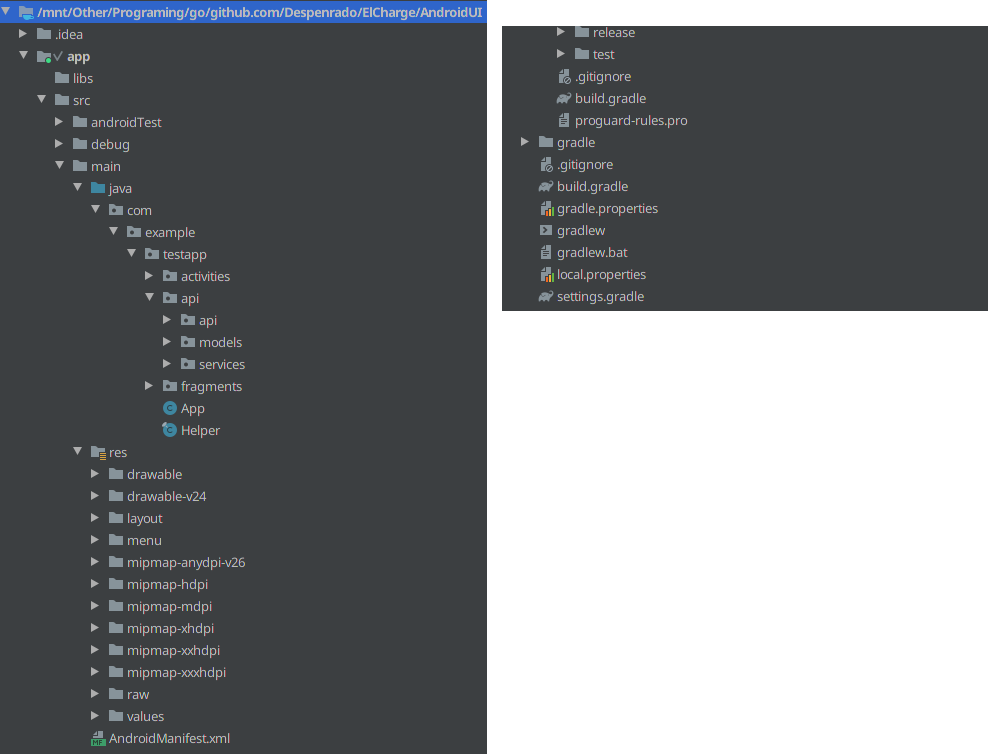
\includegraphics[width=0.4\linewidth]{rys03/frontend_file_struct.png}
\caption{Struktura plików aplikacji mobilnej}
\label{fig:frontend_file_structure}
\end{figure}

Zawartość znaczących katalogów i plików:
\begin{itemize}
    \item katalog \texttt{main/java/com/example/testapp/activities} zawiera klasy \texttt{activity}, są oknami aplikacji, na których umieszczone wszystkie komponenty interfejsu użytkownika.
    \item katalog \texttt{main/java/com/example/testapp/api} zawiera modeli danych (\texttt{katalog models}, sposób komunikacji z częścią serwerową (katalog \texttt{services}) oraz endpointy do połączenia (katalog \texttt{api} \ref{fig:frontend_file_structure_1}a).
    \item katalog \texttt{main/java/com/example/testapp/fragments} zawiera klasy fragmentów (fig. \ref{fig:frontend_file_structure_1}b), które umieszczają się w kontenerze na \texttt{activity} i zawierają elementy interfejsu użytkownika (przyciski, pola tekstowe i inne).
    \item w katalogu \texttt{res} znajdują się zasoby aplikacji, na przykład: plik konfiguracyjny (\texttt{res/raw/config.properties}), opisy komponentów oraz ich dyslokacja na fragmentach i oknach aplikacji (\texttt{res/layout/}) \ref{fig:frontend_file_structure_1}c.
    \item plik \texttt{main/androidManifest.xml} (listing \ref{list:androidManifest}) zawiera informację niezbędną do budowy aplikacji: definiowanie \texttt{activity}, uprawnień, klasy podstawowej.
    \item plik \texttt{main/java/com/example/testapp/App.java} jest klasą podstawową, który jest niezbędny do podtrzymywania globalnego stanu aplikacji (\texttt{ApplicatioContext}).
\end{itemize}
\begin{figure}[ht]
	\centering
    \begin{tabular}{@{}rl@{\hspace{3mm}}rl@{\hspace{3mm}}rl@{}}
        a) & \vtop{\vskip-2ex\hbox{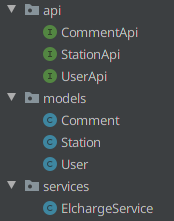
\includegraphics[width=0.253\linewidth]{rys03/frontend_file_struct_api.png}}} &
        b) & \vtop{\vskip-2ex\hbox{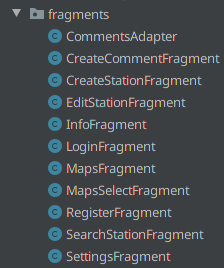
\includegraphics[width=0.27\linewidth]{rys03/frontend_file_struct_fragements.png}}} &
        c) & \vtop{\vskip-2ex\hbox{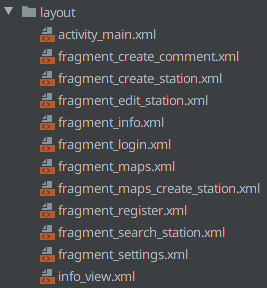
\includegraphics[width=0.30\linewidth]{rys03/frontend_file_struct_layout.png}}}
    \end{tabular}
    \caption{Struktura plików: a) API do połączenia z serwerem, b) klasy fragmentów, c) opis fragmentów.}
    \label{fig:frontend_file_structure_1}
\end{figure}
\begin{lstlisting}[label=list:androidManifest,caption=androidManifest.xml,basicstyle=\tiny\ttfamily]
    <?xml version="1.0" encoding="utf-8"?>
    <manifest xmlns:android="http://schemas.android.com/apk/res/android"
        package="com.example.testapp">
    
        <uses-permission android:name="android.permission.ACCESS_FINE_LOCATION" />
        <uses-permission android:name="android.permission.ACCESS_COARSE_LOCATION" />
        <uses-permission android:name="android.permission.INTERNET" />
        <uses-permission android:name="android.permission.ACCESS_NETWORK_STATE" />
        <uses-permission android:name="android.permission.READ_EXTERNAL_STORAGE" />
        <uses-permission android:name="android.permission.WRITE_EXTERNAL_STORAGE"/>
    
        <application
            android:name=".App"
            android:allowBackup="true"
            android:icon="@mipmap/ic_launcher"
            android:label="@string/app_name"
            android:roundIcon="@mipmap/ic_launcher_round"
            android:supportsRtl="true"
            android:theme="@style/AppTheme"
            android:usesCleartextTraffic="true">
            <meta-data
                android:name="com.google.android.geo.API_KEY"
                android:value="@string/google_maps_key" />
    
            <activity android:name=".activities.MainActivity">
                <intent-filter>
                    <action android:name="android.intent.action.MAIN" />
    
                    <category android:name="android.intent.category.LAUNCHER" />
                </intent-filter>
            </activity>
        </application>
    
    </manifest>
\end{lstlisting}

\paragraph{Modeli danych:} \texttt{User} \ref{list:user_class}, \texttt{Station} \ref{list:station_class}, \texttt{Comment} \ref{list:comment_class}. W listingach komentarz \texttt{// GETTERS and SETTERS} pokazuje, że w kodzie programu tym miejscu znajdują się proste metody do zapisu i wczytania pól klasy.
Adnotacja \texttt{@SerializedName} ustala nazwę do dekodowania do formatu JSON i naodwrót.

\begin{lstlisting}[label=list:user_class,caption=Plik \texttt{main/java/com/example/testapp/api/api/UserApi.java},basicstyle=\tiny\ttfamily]
    public class User {
        @SerializedName("_id")
        private String id;
        @SerializedName("user_name")
        private String userName;
        @SerializedName("email")
        private String email;
        @SerializedName("password")
        private String password;
        @SerializedName("update_at")
        private String updateAt;
    
        public User() {
        }
    
        public User(String id, String userName, String email, String password, String updateAt) {
            this.id = id;
            this.userName = userName;
            this.email = email;
            this.password = password;
            this.updateAt = updateAt;
        }
        // GETTERS and SETTERS
    }
\end{lstlisting}

\begin{lstlisting}[label=list:station_class,caption=Plik \texttt{main/java/com/example/testapp/api/api/StationApi.java},basicstyle=\tiny\ttfamily]
    public class Station {
        @SerializedName("_id")
        private String id;
        @SerializedName("owner_id")
        private String ownerID;
        @SerializedName("description")
        private String description;
        @SerializedName("station_name")
        private String stationName;
        @SerializedName("latitude")
        private double latitude;
        @SerializedName("longitude")
        private double longitude;
        @SerializedName("update_at")
        private String updateAt;
        @SerializedName("rating")
        private float rating;
        @SerializedName("comments")
        private ArrayList<Comment> comments;
    
        public Station() {
        }
    
        public Station(String id, String ownerID, String description, String stationName, double latitude, double longitude, String updateAt, float rating, ArrayList<Comment> comments) {
            this.id = id;
            this.ownerID = ownerID;
            this.description = description;
            this.stationName = stationName;
            this.latitude = latitude;
            this.longitude = longitude;
            this.updateAt = updateAt;
            this.rating = rating;
            this.comments = comments;
        }
        // GETTERS and SETTERS
    }
\end{lstlisting}

\begin{lstlisting}[label=list:comment_class,caption=Plik \texttt{main/java/com/example/testapp/api/api/CommentApi.java},basicstyle=\tiny\ttfamily]
    public class Comment {
        @SerializedName("_id")
        private String id;
        @SerializedName("user_id")
        private String userID;
        @SerializedName("user_name")
        private String userName;
        @SerializedName("text")
        private String text;
        @SerializedName("rating")
        private float rating;
        @SerializedName("create_at")
        private String createAt;
        @SerializedName("update_at")
        private String updateAt;
    
        public Comment() {
        }
    
        public Comment(String id, String userID, String userName, String text, float raiting, String createAt, String updateAt) {
            this.id = id;
            this.userID = userID;
            this.userName = userName;
            this.text = text;
            this.rating = raiting;
            this.createAt = createAt;
            this.updateAt = updateAt;
        }
        // GETTERS and SETTERS
    }
\end{lstlisting}

\paragraph{API:} \texttt{UserApi} \ref{list:android_api_user}, \texttt{StationApi} \ref{list:android_api_station}, \texttt{CommentApi} \ref{list:android_api_comment} są interfejsami do komunikacji przez interfejsy programistyczne z częścią serwerową.
Adnotacje \texttt{POST}, \texttt{PU}, \texttt{GET}, \texttt{DELETE} wskazują na to, którą metodą należy wysłać zapytania do części serwerowej.
Adnotacja \texttt{Body} umieszcza dane do ciała zapytania. Adnotacje \texttt{Path} umieszcza dane jako część adresu URL. Adnotacje \texttt{Query} umieszcza dane jako odpowiednie parametry w adresie URL.

\begin{lstlisting}[label=list:android_api_user,caption=Plik \texttt{main/java/com/example/testapp/api/api/UserApi.java},basicstyle=\tiny\ttfamily]
    public interface UserApi {
        @POST("users")
        public Single<Response<User>> createUser(@Body User body);
    
        @POST("login")
        public Single<Response<User>> login(@Body User body);
    
        @GET("logout/{id}")
        public Single<ResponseBody> logout(@Path("id") String id);
    }
\end{lstlisting}

\begin{lstlisting}[label=list:android_api_station,caption=Plik \texttt{main/java/com/example/testapp/api/api/StationApi.java},basicstyle=\tiny\ttfamily]
    public interface StationApi {

        @POST("stations")
        public Single<Response<Station>> createStation(@Body Station station);
    
        @GET("stations/read")
        public Single<Response<List<Station>>> readStationsByLatAndLngAndDist(@Query("skip") int skip, @Query("limit") int limit, @Query("lat") double lat, @Query("lng") double lng, @Query("dist") int dist);
    
        @GET("stations/read")
        public Single<Response<Station>> readStationsByLatAndLng(@Query("skip") int skip, @Query("limit") int limit, @Query("lat") double lat, @Query("lng") double lng);
    
        @GET("stations/read")
        public Single<Response<List<Station>>> readStationsByDescription(@Query("skip") int skip, @Query("limit") int limit, @Query("descr") String descr);
    
        @GET("stations/read")
        public Single<Response<List<Station>>> readStationsByName(@Query("skip") int skip, @Query("limit") int limit, @Query("name") String name);
    
        @GET("stations/read")
        public Single<Response<List<Station>>> readStations(@Query("skip") int skip, @Query("limit") int limit);
    
        @GET("stations/{id}")
        public Single<Response<Station>> findById(@Path("id") String id);
    
        @PUT("stations/{id}")
        public Single<Response<Station>> updateById(@Path("id") String id, @Query("ownid") String ownid, @Body Station station);
    
        @DELETE("stations/{id}")
        public Single<ResponseBody> deleteById(@Path("id") String id);
    }
\end{lstlisting}

\begin{lstlisting}[label=list:android_api_comment,caption=Plik \texttt{main/java/com/example/testapp/api/api/CommentApi.java},basicstyle=\tiny\ttfamily]
    public interface CommentApi {
        @POST("stations/{sid}/comments")
        public Single<Response<Comment>> createComment(@Path("sid") String sid, @Body Comment comment);
    
        @GET("stations/{sid}/comments/read")
        public Single<Response<List<Comment>>> readComments(@Path("sid") String sid, @Query("skip") int skip, @Query("limit") int limit);
    
        @GET("stations/{sid}/comments/{id}")
        public Single<Response<Comment>> findById(@Path("sid") String sid, @Path("id") String id);
    
        @PUT("stations/{sid}/comments/{id}")
        public Single<Response<Comment>> updateById(@Path("sid") String sid, @Path("id") String id, @Body Comment comment);
    
        @DELETE("stations/{sid}/comments/{id}")
        public Single<ResponseBody> deleteById(@Path("sid") String sid, @Path("id") String id);
    }
\end{lstlisting}

\subsubsection{?? Działanie interfejsu graficznego ??}

\subsection{Funkcje aplikacji mobilnej}
W tej sekcji opisano współdziałanie użytkownika i systemu oraz implementacja tych części.

\subsubsection{Autentykacja / Logowanie i rejestracja}
Dla otwarcia strony logowania lub rejestracji można nacisnąć przycisk w prawym dolnym rogu (koło zębate). Otworzą się ustalenia, jak na rysunku \ref{fig:}, oraz kliknąć \texttt{Log in} (na tej stronie można też wylogować się za pomocą przycisku \texttt{Log out}).
Przy próbie wykorzystania elementów, które potrzebują autentykacji, natomiast użytkownik nie będzie zalogowany do systemu, logowanie \ref{fig:} oraz rejestracja \ref{fig:} będą proponowane automatycznie. Jeśli logowanie zostało proponowane automatycznie, dane poprzedniego ekranu nie będą usuwane, więc po zalogowaniu się można kontynuować pracę.


\subsubsection{Stacja}
\paragraph{Dodawanie}
\paragraph{Wczytywanie}
\paragraph{Edycja}
\subsubsection{Komentarz}
\paragraph{Dodawanie}
\paragraph{Wczytywanie}

\chapter{Testy}
\label{ch:Testy}
W niniejszym rozdzialie zostały przedstawione listy przeprowadzonych testów oraz kilka ich przykładów.
\section{Testy jednostkowe}
% % Для проведения тестов серверной части достаточно выпонить команду \texttt{make test} в папке 'RestAPI'.
% % Для тестирования использовались библиотка stretchr/testify.
% % Файлы преднозначенные для тестирования находятся рядом с тестируеммыми файлами. Они отличаются от вайлов приложения названием: '*\_test.go'.
% % Код показывает пример тестирования валидации данных для сущности пользователя, которое используется, напривер, перед добавлением пользователя в базу данных:
Aby przeprowadzić testy po stronie serwera, wystarczy uruchomić polecenie \texttt{make test} w folderze 'RestAPI'.
Do testowania użyto biblioteki ,,stretchr/testify''.
Pliki przeznaczone do testowania znajdują się obok testowanych plików. Różnią się one od plików aplikacji nazwą: *\_test.go.

Kod \ref{list:test_user_valitation} pokazuje przykład testowania walidacji danych dla jednostki użytkownika, która jest używana na przykład przed dodaniem użytkownika do bazy danych.
\begin{lstlisting}[label=list:test_user_valitation,caption=Kod testowania walidacji danych użytkownika,basicstyle=\tiny\ttfamily]
    func TestValidate(t *testing.T) {
        testCase := []struct {
            name    string
            user    *User
            isValid bool
        }{
            {
                name: "simple",
                user: &User{
                    UserName: "valid",
                    Email:    "valid@email.com",
                    Password: "validpass",
                },
                isValid: true,
            },
            {
                name: "without username",
                user: &User{
                    Email:    "valid@email.com",
                    Password: "validpass",
                },
                isValid: true,
            },
            {
                name: "without email",
                user: &User{
                    UserName: "valid",
                    Password: "validpass",
                },
                isValid: false,
            },
            {
                name: "without password",
                user: &User{
                    UserName: "valid",
                    Email:    "valid@email.com",
                },
                isValid: false,
            },
            {
                name: "wrong email",
                user: &User{
                    UserName: "valid",
                    Email:    "wrong",
                    Password: "validpass",
                },
                isValid: false,
            },
            {
                name: "wrong password",
                user: &User{
                    UserName: "valid",
                    Email:    "valid@email.com",
                    Password: "wrong",
                },
                isValid: false,
            },
            {
                name: "wrong username",
                user: &User{
                    UserName: "n",
                    Email:    "valid@email.com",
                    Password: "validpass",
                },
                isValid: false,
            },
        }
    
        for _, item := range testCase {
            t.Run(item.name, func(t *testing.T) {
                if item.isValid {
                    assert.NoError(t, item.user.Validate())
                } else {
                    assert.Error(t, item.user.Validate())
                }
            })
        }
    }
\end{lstlisting}

% Для тестирования функций, которые не требуют прямого подлючения к MongoDB, используется пакет-заглушка 'storage/teststorage' с базой данных в виде карты ключ-значение. Тесты взаимодеййствия с реальной базой даннх также проведены.
Do testowania funkcji, które nie wymagają bezpośredniego połączenia z MongoDB, używany jest pakiet ,,storage/teststorage'' z bazą danych zaimplementowanej jako mapa klucz-wartość. Przeprowadzono również testy interakcji z rzeczywistą bazą danych.

% Примером тестирования создания пользователя в базе данных служит код:
Przykładem testowania tworzenia użytkownika w bazie danych jest kod \ref{list:test_mongoDB}:
\begin{lstlisting}[label=list:test_mongoDB,caption=Kod testowania tworzenia użytkownika w MongoDB,basicstyle=\tiny\ttfamily]
    func TestCreate(t *testing.T) {
        ur := testHelperUser()
        ti := models.GetTimeNow()
        user := &models.User{
            UserName: "username_1",
            Email:    "1@email.com",
            Password: "passwoed_1",
            Model: models.Model{
                UpdateAt: ti,
                CreateAt: ti,
            },
        }
        id, err := ur.Create(user)
        assert.Nil(t, err)
        assert.NotEqual(t, id, "")
        ur.DeleteByID(id)
    }
\end{lstlisting}

% Пример тестирования создания пользователя в фиктивонй базе данных:
Przykład testowania tworzenia użytkownika w fikcyjnej bazie danych \ref{list:test_fictive}.
\begin{lstlisting}[label=list:test_fictive,caption=Kod testowania tworzenia użytkownika w fikcyjnej bazie danych,basicstyle=\tiny\ttfamily]
    func TestCreate(t *testing.T) {
        ur := NewUserRepository()
        ti := models.GetTimeNow()
        user := &models.User{
            UserName: "username_1",
            Email:    "1@email.com",
            Password: "passwoed_1",
            Model: models.Model{
                UpdateAt: ti,
                CreateAt: ti,
            },
        }
        id, err := ur.Create(user)
        assert.Nil(t, err)
        assert.NotEqual(t, id, "")
        user.ID = id
        assert.Equal(t, ur.db[id], user)
    }
\end{lstlisting}

% Список всех файлов тестирования (создан с помощью плагина для Visual Studio Code 'ethan-reesor.vscode-go-test-adapter')
Lista wszystkich testów jednostkowych znajduje się na rysunku \ref{fig:test_list}.
% TO DO: proszę przycinać rysunki, by nie miały białych marginesów
\begin{figure}[ht]
    \centering
        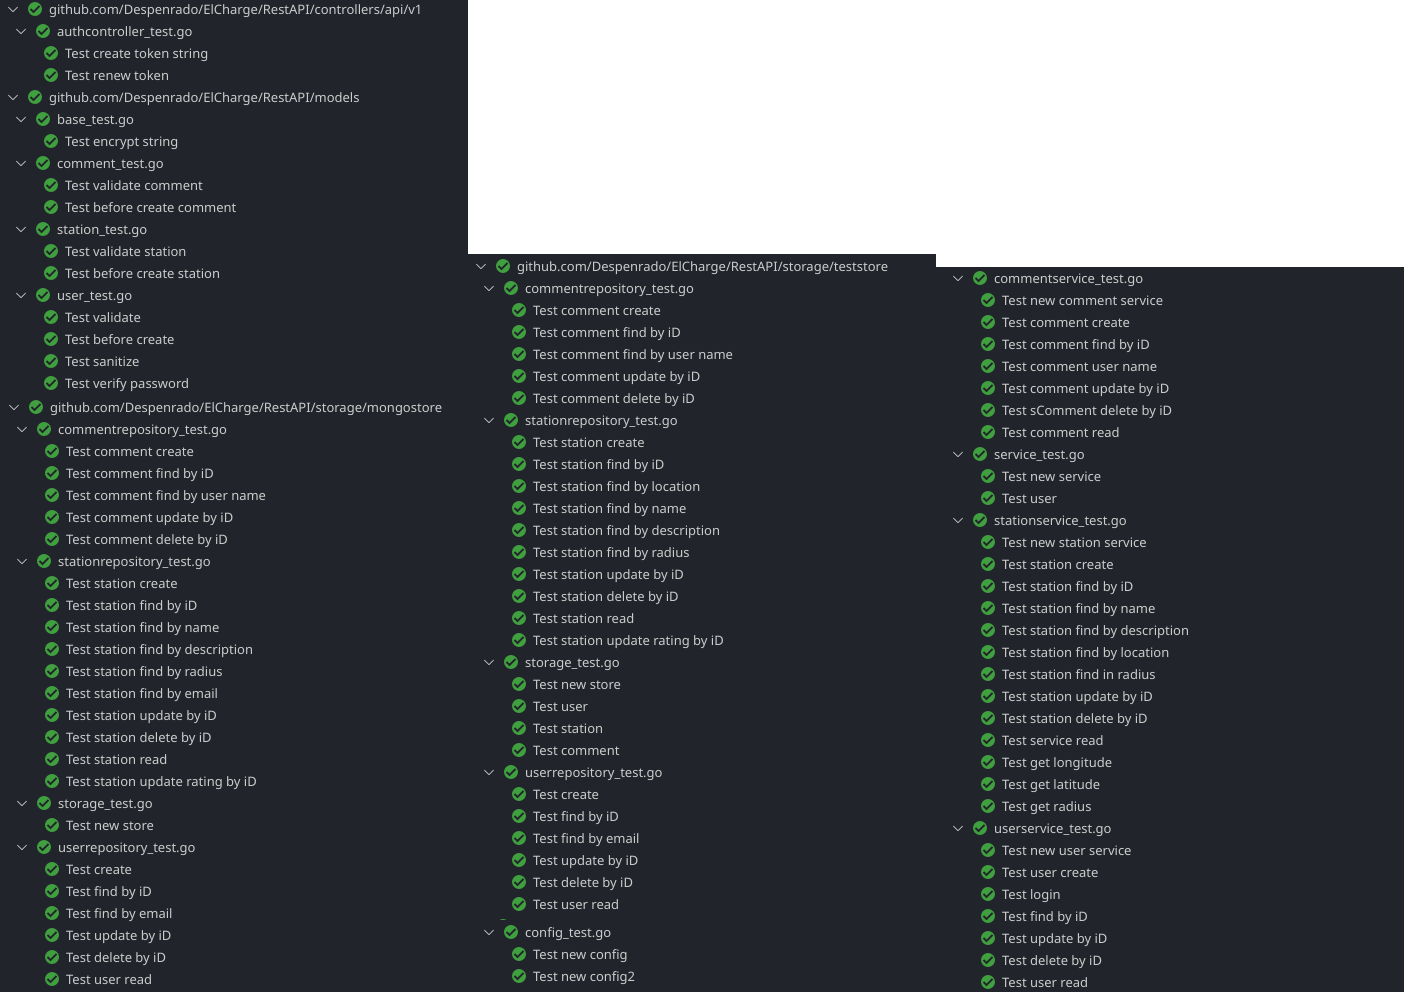
\includegraphics[width=1\linewidth]{rys04/test_list.png}
        \caption{Lista testów jednostkowych}
    \label{fig:test_list}
\end{figure}

% 
\section{Testy API}
Do testowania interfejsu API wykorzystano narzędzie do automatycznego testowania Postman.
Przeprowadzono testy wszystkich endpointów (rys. \ref{fig:postma_list}).
\begin{figure}[ht]
    \centering
        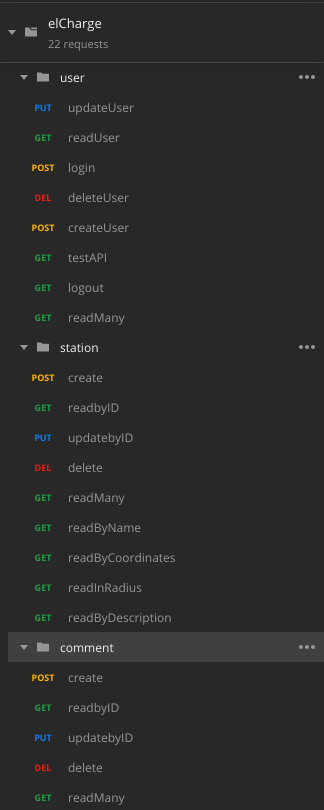
\includegraphics[width=0.3\linewidth]{rys04/postman_list.png}
        \caption{Lista testów API}
    \label{fig:postma_list}
\end{figure}
\newpage

Przykład testowania logowania (rys. \ref{fig:postman_login1}):
\begin{figure}[ht]
    \centering
        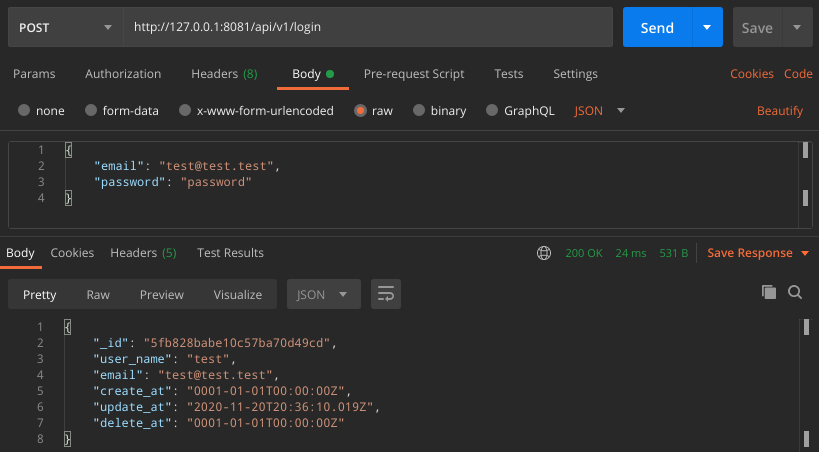
\includegraphics[width=1\linewidth]{rys04/postman_login1.png}
        \caption{Testowanie logowania za pomocą Postman}
    \label{fig:postman_login1}
\end{figure}

% TO DO: proszę zrzuty z Postmana robić przy zawężonym oknie (okienko nie może rozpinać się na całą szerokość ekranu, bo potem jak się wklei obrazek do dokumentu wychodzą za małe literki).
Przykład testowania tworzenia stacji ładującej samochody elektryczne (rys. \ref{fig:postman_create_station}).
\begin{figure}[ht]
    \centering
        \includegraphics[width=1\linewidth]{rys04/postman_create_station.png}
        \caption{Testowanie tworzenia stacji ładowanicej za pomocą Postman}
    \label{fig:postman_create_station}
\end{figure}

% Пример создания еомментария и его модификции.
Przykład tworzenia komentarza (rys. \ref{fig:postman_create_comment}) i jego modyfikacji (rys. \ref{fig:postman_edit_comment}).
\begin{figure}[ht]
    \centering
        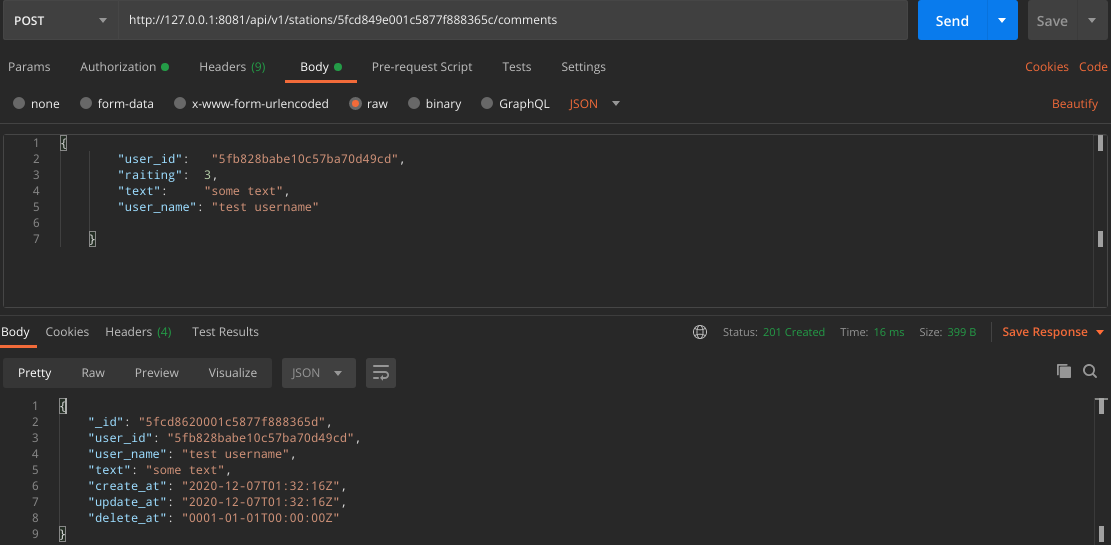
\includegraphics[width=0.9\linewidth]{rys04/postman_create_comment.png}
        \caption{Testowanie tworzenia komentarza za pomocą Postman}
    \label{fig:postman_create_comment}
\end{figure}
\begin{figure}[ht]
    \centering
        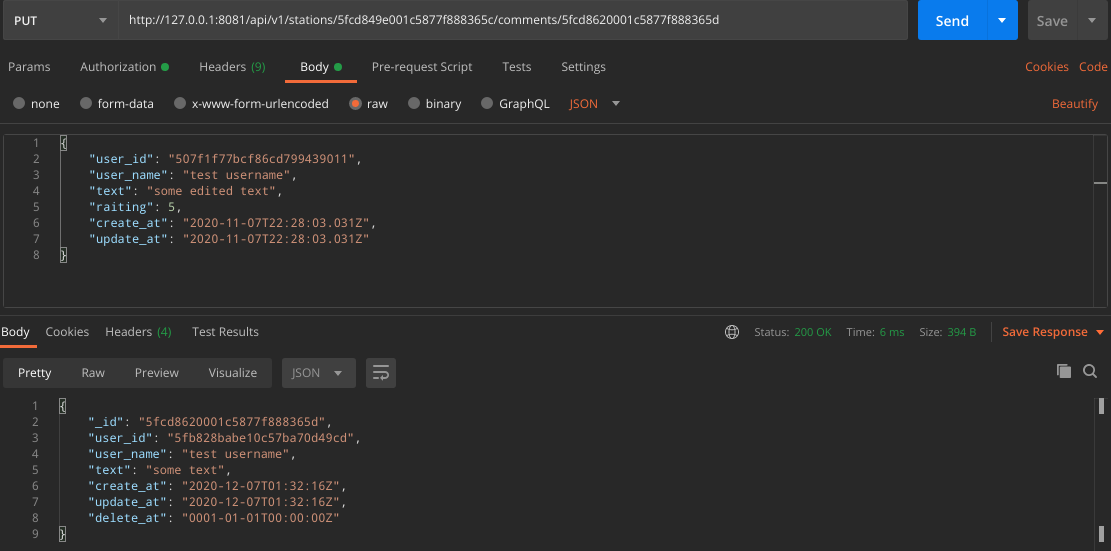
\includegraphics[width=0.9\linewidth]{rys04/postman_edit_comment.png}
        \caption{Testowanie edycji komentarza za pomocą Postman}
    \label{fig:postman_edit_comment}
\end{figure}
\newpage
% пример поиска зарядной станции в радиусе 100 км от установлиенных координат, а также лиммитирования списка:
Przykład wyszukiwania stacji ładującej (rys. \ref{fig:postman_find_stations}) w dystansie 100 km od ustalonych współrzędnych, a także ograniczenia listy:
\begin{figure}[ht]
    \centering
        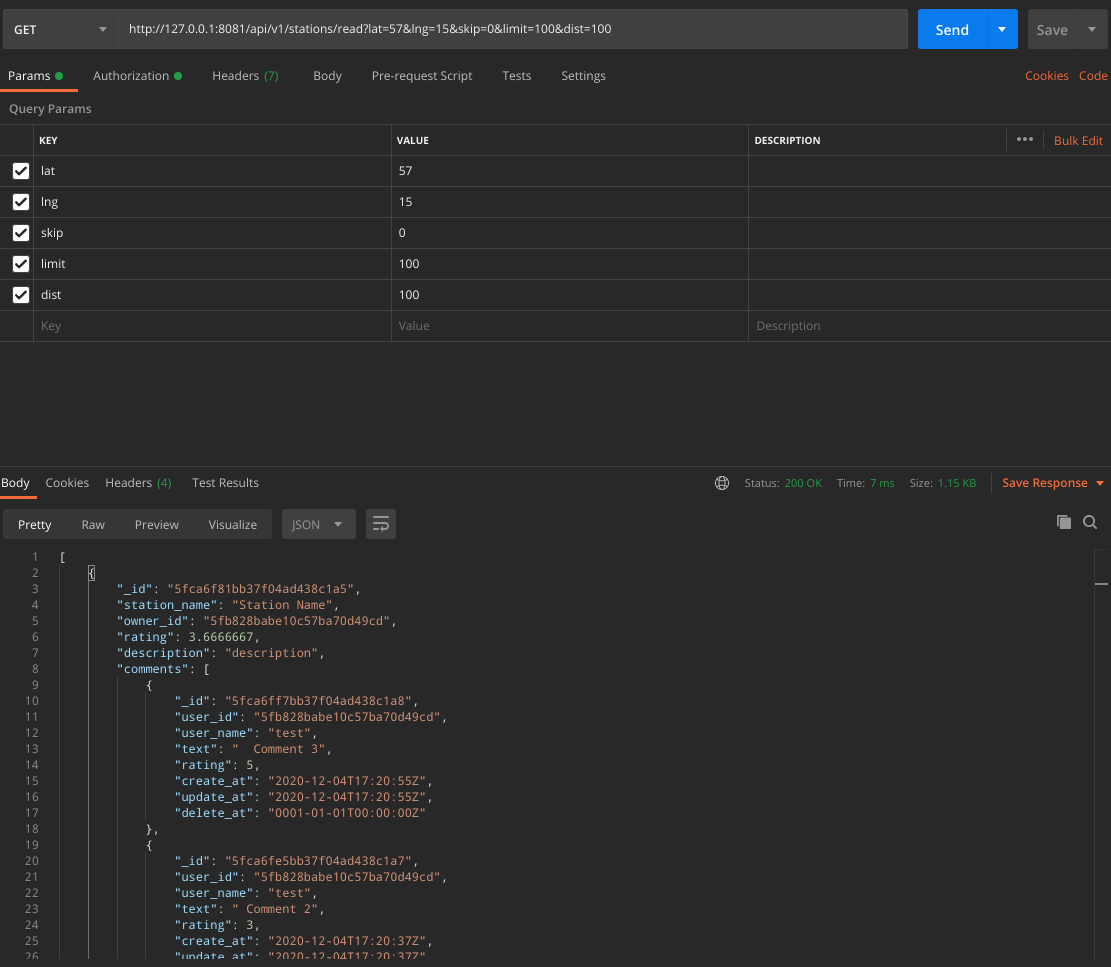
\includegraphics[width=0.9\linewidth]{rys04/postman_find_stations.png}
        \caption{Testowanie złożonego wyszukiwania stacji ładowniczej za pomocą Postman}
    \label{fig:postman_find_stations}
\end{figure}
% \chapter{Wdrożenie części serwerowej}
\paragraph{RestAPI}
% Для развертывая серверной части вместе с базами данных MongoDB и Redis достаточно двух комманд.
% Должны быть установлены docker и docker-compose.

% Первая команда создает 3 образа: образ базы даннх MongoDB, образ базы данных Redis и образ серверной части приложения написаной на Go:
Do wdrożenia części serwerowej wraz z bazami danych MongoDB i Redis wystarczy wykonać dwa polecenia.
Musi być zainstalowany docker i Docker-compose.

Pierwsze polecenie tworzy 3 obrazy: obraz bazy danych dunnh MongoDB, Obraz bazy danych Redis i obraz zaplecza aplikacji napisany w Go:

\texttt{\$ docker-compose build}
% Вторая команда запускает созданные ранее образы в оперделенной последовательности, а также создает каналы для взаимодействия приложений из контейнеров.
Drugie polecenie uruchamia wcześniej utworzone obrazy w określonej kolejności, a także tworzy kanały do interakcji części aplikacji między kontenerami oraz środowyskiem wewnętrznym.

\texttt{\$ docker-compose up}

% Для управления контейнерами ипользуется файл docker-compose:
Do zarządzania kontenerami służy plik \texttt{docker-compose.yml} \ref{list:docker-compose.yml}:
\begin{lstlisting}[label=list:docker-compose.yml,caption=docker-compose.yml,basicstyle=\tiny\ttfamily]
    version: "3.5" # Use version 3.5 syntax
    services: # Here we define our service(s)
        db:
            container_name: mongoDB-elcharge # Container name
            image: mongo # image name to start/build
            ports: # Port mapping
                - "2717:27017"
            volumes: # Volume binding
                - "~/example:/data/db"
        cache-db:
            container_name: redis-elcharge # Container name
            image: redis
            ports:
                - "63799:6379"
            volumes: # Volume binding
                - "/opt/redis/data:/data"
        golang-restapi: # The name of the service
            build:
                context: .
                dockerfile: Dockerfile # Location of our Dockerfile
            image: despenrado/golang-restapi-elcharge:prod.0.1
            container_name: restapi-elcharge # Container name
            depends_on: # start after
                - cache-db
                - db
            ports:
                - "8081:8081"
            links: # list mapping: service_name:name_how_will_see_your_program
                - "db:mymongo"
                - "cache-db:myredis"
    
\end{lstlisting}

% Для этапов устновки зависимостей, компиляции и самого создания образа серверной части приложения использется Dockerfile:
Plik Dockerfile \ref{list:dockerfile} jest używany do etapów instalacji zależności, kompilacji i samego tworzenia obrazu zaplecza aplikacji:
\begin{lstlisting}[label=list:dockerfile,caption=Dockerfile,basicstyle=\tiny\ttfamily]
    FROM golang:1.15 AS builder
    WORKDIR /go/src/github.com/Ddespenrado/ElCharge/RestAPI/
    COPY . .
    RUN go mod tidy
    RUN CGO_ENABLED=0 GOOS=linux GOARCH=amd64 go build -a -tags netgo -ldflags '-w' -o restapi .
    
    FROM scratch
    EXPOSE 8081
    WORKDIR /root/
    COPY deploy/apiserver.yaml .
    COPY --from=builder /go/src/github.com/Ddespenrado/ElCharge/RestAPI/restapi .
    ENTRYPOINT ["./restapi","-config=apiserver.yaml"]
\end{lstlisting}

Plikiem konfiguracyjnym aplikacji, w przypadku używania dockera jest plik \texttt{RestAPI/deploy/apiserver.yaml}.
\chapter{Podsumowanie}
W tym rozdziale znajują się wnioski i plany na rozwój aplikacji.

\section{Wnioski}
% В этом проекте планировалось решить проблему с поиском зарядных станций для автомобилей. Должно было быть создано мобильное приложение, в которм пользователь может не только быстро и удобно искать походящую ему станцию, но и добавлять новые, еще не отмеченные на карте.
% Это позволило бы создать самодостаточное приложение, для которого не требовалось бы больших вложений для поддержания инфраструктуры. Приложение должно было позволить создавать коментарии и выставлять оценку зарядным станциям. Для удобства поиска должна была использоваться карта.
% На карте, кроме зарядных станций должна была отмечаться в том числе позиция пользователя.

% В приложени были реализованы все представленные выше функции, однако в процессе разработки были выявлены некоторые недостатки, о которых будет оговорено в планах на будущее. 

% Благодаря выбранныой базе данных MongoDB приложение можно легко расширять. Также все выбранные технологии оказались очень гибкими и прспособленными для этой задачи.
% Самым полезным источником информации стала официальная документация доступная на страницах \cite{android_doc,godoc,golang2,mongoDB_doc}. Книга по языку Go \cite{LearninGo}. Книга по языку Java \cite{javabook}
% % 
W tym projekcie planowano rozwiązać problem ze znalezieniem stacji ładowania pojazdów elektrycznych. Miała zostać stworzona aplikacja mobilna, w której użytkownik może nie tylko szybko i wygodnie wyszukiwać stację ładownicze, które mu odpowiadają, ale także dodawać nowe, których jeszcze nie ma w systemie.
Umożliwiłoby to stworzenie samowystarczalnej aplikacji, która nie wymagałaby dużych inwestycji w celu utrzymania infrastruktury. Aplikacja miała umożliwić tworzenie komentarzy i ocenianie stacji ładowania pojazdów elekrycznych. Dla ułatwienia wyszukiwania miała być użyta mapa.
Na mapie oprócz stacji ładowania miała być zaznaczona m.in. pozycja użytkownika.

W aplikacji zostały zaimplementowane wszystkie powyższe funkcje, ale w procesie rozwoju zidentyfikowano pewne niezbędne funkcjalności, które zostaną określone w planach \ref{sec:plany} na przyszłość.

Dzięki wybranej bazie danych MongoDB aplikacja może być łatwo rozbudowywana o nowe kolekcje i zmienione już istniejące. Wszystkie wybrane technologie okazały się bardzo elastyczne i odpowiednie przystosowane do tego zadania.
Najbardziej użytecznym źródłem informacji była oficjalna dokumentacja wybranych nażędzi \cite{android_doc,godoc,golang2,mongoDB_doc}. Też była użyteczna książka o języku Go \cite{LearninGo} oraz książka o języku Java \cite{javabook}
%
\section{Plany}
\label{sec:plany}
% % 
% Безопасность: 
% \begin{itemize}
%     \item Создание панели администратора для модерации комментариев;
%     \item Закрытие доступа любого авторезированого пользователя к данным, которые не разрешены через мобильное приложение.
% \end{itemize}

% Удобство пользования: 
% \begin{itemize}
%     \item Добавление возможности удаления комментариев через мобильное приложение;
%     \item Расширение возможностей работы с картой с помощью сервисов google cloud. Например прокладывание маршрута;
% \end{itemize}
Bezpieczeństwo:
\begin{itemize}
    \item Tworzenie panelu admina do moderacji komentarzy;
    \item Zamknięcie dostępu dowolnego użytkownika do danych, które nie są dozwolone za pośrednictwem aplikacji mobilnej, to znaczy zamknięcie API;
    \item Uleprzenie niektórych endpointów, na przykład sposobu wyszukiwania wedłóg parametrów w endpoincie \texttt{/api/v1/stations/read?skip=""\&limit=""\&lat=""\&lng=""\&dist=""\&descr=""\&nam=""}.
\end{itemize}

Wygoda użytkowania aplikacją:
\begin{itemize}
    \item Dodawanie możliwości usuwania komentarzy za pośrednictwem aplikacji mobilnej;
    \item Rozszerzenie możliwości pracy z mapą za pomocą usług google cloud. Na przykład wyznaczanie trasy;
\end{itemize}

%\bibliographystyle{plalpha}
\bibliographystyle{plabbrv}

%UWAGA: bibliotekę referencji należy przygotować samemu. Dobrym do tego narzędziem jest JabRef.
%       Nazwę przygotowanej biblioteki wpisuje się poniżej bez rozszerzenia 
%       (w tym przypadku jest to "dokumentacja.bib")
\setlength{\bibitemsep}{2pt} % - by zacieśnić wykaz literatury
\bibliography{dokumentacja}
\appendix
\chapter{Opis załączonej płyty CD/DVD}
Tutaj jest miejsce na zamieszczenie opisu zawartości załączonej płyty.
Należy wymienić, co zawiera.
\chapter{Wdrożenie aplikacji}
\section{Wdrożenie części serwerowej}
\paragraph{RestAPI}
% Для развертывая серверной части вместе с базами данных MongoDB и Redis достаточно двух комманд.
% Должны быть установлены docker и docker-compose.

% Первая команда создает 3 образа: образ базы даннх MongoDB, образ базы данных Redis и образ серверной части приложения написаной на Go:
Do wdrożenia części serwerowej wraz z bazami danych MongoDB i Redis wystarczy wykonać dwa polecenia.
Musi być zainstalowany Docker i Docker-compose.

Pierwsze polecenie tworzy 3 obrazy: obraz bazy danych dunnh MongoDB, obraz bazy danych Redis i obraz serwerowej części aplikacji napisanej w języku Go:

\texttt{\$ docker-compose build}

% Вторая команда запускает созданные ранее образы в оперделенной последовательности, а также создает каналы для взаимодействия приложений из контейнеров.
Drugie polecenie uruchamia wcześniej utworzone obrazy w~określonej kolejności, a także tworzy kanały do interakcji części aplikacji między kontenerami oraz środowyskiem wewnętrznym.

\texttt{\$ docker-compose up}

% Для управления контейнерами ипользуется файл docker-compose:
Do zarządzania kontenerami służy plik \texttt{docker-compose.yml} \ref{list:docker-compose.yml}:
\begin{lstlisting}[label=list:docker-compose.yml,caption=docker-compose.yml,basicstyle=\tiny\ttfamily]
    version: "3.5" # Use version 3.5 syntax
    services: # Here we define our service(s)
        db:
            container_name: mongoDB-elcharge # Container name
            image: mongo # image name to start/build
            ports: # Port mapping
                - "2717:27017"
            volumes: # Volume binding
                - "~/example:/data/db"
        cache-db:
            container_name: redis-elcharge # Container name
            image: redis
            ports:
                - "63799:6379"
            volumes: # Volume binding
                - "/opt/redis/data:/data"
        golang-restapi: # The name of the service
            build:
                context: .
                dockerfile: Dockerfile # Location of our Dockerfile
            image: despenrado/golang-restapi-elcharge:prod.0.1
            container_name: restapi-elcharge # Container name
            depends_on: # start after
                - cache-db
                - db
            ports:
                - "8081:8081"
            links: # list mapping: service_name:name_how_will_see_your_program
                - "db:mymongo"
                - "cache-db:myredis"
    
\end{lstlisting}

% Для этапов устновки зависимостей, компиляции и самого создания образа серверной части приложения использется Dockerfile:
Plik Dockerfile \ref{list:dockerfile} jest używany do etapów instalacji zależności, kompilacji i samego tworzenia obrazu zaplecza aplikacji:
\begin{lstlisting}[label=list:dockerfile,caption=Dockerfile,basicstyle=\tiny\ttfamily]
    FROM golang:1.15 AS builder
    WORKDIR /go/src/github.com/Ddespenrado/ElCharge/RestAPI/
    COPY . .
    RUN go mod tidy
    RUN CGO_ENABLED=0 GOOS=linux GOARCH=amd64 go build -a -tags netgo -ldflags '-w' -o restapi .
    
    FROM scratch
    EXPOSE 8081
    WORKDIR /root/
    COPY deploy/apiserver.yaml .
    COPY --from=builder /go/src/github.com/Ddespenrado/ElCharge/RestAPI/restapi .
    ENTRYPOINT ["./restapi","-config=apiserver.yaml"]
\end{lstlisting}

Plikiem konfiguracyjnym aplikacji, w przypadku używania dockera jest plik \texttt{RestAPI/deploy/apiserver.yaml}.


\section{Instalacja i uruchomienie aplikacji mobilnej}
Najpierw trzeba skopiować plik \texttt{elCharge.apk} do urządzenia z systemem Android, znaleźć ten plik, otworzyć (kliknąć na niego) oraz zgodzić się na instalację.
Uruchomić aplikację \texttt{TestApp}.

W przypadku uruchomiania za pomocą emulatora, wbudowanego w Android Studio, należy mieć zainstalowany Android Studio oraz Java SDK 8.
Należy otworzyć katalog \texttt{AndroidUI} za pomocą Android Studio, wybrać emulator z systemem Android powyżej wersji 4.1 i uruchomić za pomocą odpowiedniego przycisku.
\chapter{Tytuł dodatku}
Szybki start (dodatek, w którym opisano podstawowy scenariusz użycia rozwiązania - by czytelnik mógł na podstawie tego opisu zacząć pracę z rozwiązaniem).

W szablonie, jaki opublikowałem na mojej stronie, znajduje się opis struktury pracy. Standardowo jest to:

    1. Wstęp
        1.1 Wprowadzenie
            (zwykle 1 - 2 strony wprowadzające w dziedzinę, gdzie mogą pojawić się cytowania (!), oraz zawierające wyjaśnienie odnośnie motywacji do podjęcia tematu)
        1.2 Cel i zakres pracy
            (zwykle 0,5 - 1,5 strony z opisem tego, co ma być zrobione - cel - do czego ma się przyczynić praca, zakres - co zostanie zrobione, by osiągnąć cel. Tutaj powinna być zgodność z tym, co napisano w karcie tematu pracy. Zresztą  z opisu z karty można skorzystać, lekko go przeredagowując)
        1.3 Układ pracy
            (zwykle jeden akapit na jeden rozdział z opisem zawartości danego rozdziału)
    2. Kolejny rozdział
        2.1 Sekcja
        2.1.1 Podsekcja
            Nienumerowana podpodsekcja
                Paragraf
     .....

    A. Zawartość dołączonej płyty CD/DVD
        (dodatek, w którym opisuje się zawartość nagranej płyty z projektem informatycznym oraz dokumentem pdf z tekstem pracy. Może tam się również pojawić instalator bądź obraz dockerowy - zależnie od wybranego sposobu wdrażania stworzonego rozwiązania. Generalnie chodzi o to, by recenzent sięgając po płytę miał możliwość oceny wyników pracy. Na płycie powinno być jakieś Readme)
    B. Instrukcja wdrożeniowa (dodatek, w którym opisano jak wdrożyć/zainstalować/uruchomić rozwiązanie)
    C. Szybki start (dodatek, w którym opisano podstawowy scenariusz użycia rozwiązania - by czytelnik mógł na podstawie tego opisu zacząć pracę z rozwiązaniem).

To, co pojawia się w kolejnych rozdziałach jest w dużej mierze sprawą indywidualną. Zwykle prace inżynierskie mają na początku jakieś założenia i teoretyczne podstawy, a dopiero potem opis implementacji, testów i podsumowanie. Generalnie połowa pracy powinna być o założeniach, połowa o implementacji (jeśli praca jest typowa).

W szczególności:
   - rozdział drugi może zawierać analizę wymagań: funkcjonalnych, niefunkcjonalnych, dziedzinowych plus makiety interfejsu użytkownika. Powinien w nim się pojawić opis architektury rozwiązania (wraz ze szkice jej zarysu). Poszczególne fragmentu opisu można zilustrować diagramami wymagań SysML, opisa przypadków użycia itp. Przy okazji można wspomnieć o przyjętej metodyce prowadzenia projektu
   - rozdział trzeci może zawierać przegląd wykorzystanych technologii (w rozdziale drugim można wymienić wymagania niefunkcjonalne, zaś w rozdziale trzecim podać detale), przy czym nie może to być kopia dostępnych manuali, ale syntetyczny opis tych bibliotek, narzędzi i innych rozwiązań, które wykorzystano w pracy.
   - rozdział czwarty może być o detalach implementacji. Tutaj wykorzystać można diagramy klas, przebiegów, stanów itp. Można też pokazywać fragmenty kodu (niedopuszczalne jest wstawianie całych kodów źródłowych - wystarczy pokazać interesujący fragment, wykropkowując rzeczy nieistotne)
   - rozdziął piąty może zawierać wyniki eksperymentów bądź testów
   - w ostatnim rozdziale powinno pojawić się podsumowanie, w którym jawnie będzie powiedziane w jakim stopniu udało się zrealizować cel pracy (zakładam, że uda się go zrealizować w 100%), jakie napotkano przeszkody i jak je pokonano, jakie są możliwe zastosowania stworzonego rozwiązania oraz jakie są potencjalne kierunki jego rozwoju.

Oczywiście tytuły i zawartość rozdziałów od drugiego do ostatniego nie są z góry narzucone. Wszystko zależy od charakteru pracy inżynierskiej i sposobu jej realizacji. Inaczej wygląda dokumentacja systemu, inaczej biblioteki, a jeszcze inaczej opracowanego jakiegoś szczególnego algorytmu. Zdarzają się prace inżynierskie, w których sam sposób prowadzenia projektu jest tematem wiodącym, a w związku z tym gdzie indziej stawia się akcenty i inaczej tytułuje kolejne rozdziały.

3. Reguły redakcyjne

    1. Praca dyplomowa powinna być napisana w  formie bezosobowej ("w pracy pokazano ..."). Taki styl przyjęto na uczelniach w naszym kraju, choć w krajach anglosaskich preferuje się redagowanie treści w pierwszej osobie.
    2. W tekście pracy można odwołać się do myśli autora, ale nie w pierwszej osobie, tylko poprzez wyrażenia typu: "autor wykazał, że ...".
    3. Odwołując się do rysunków i tabel należy używać zwrotów typu: "na rysunku pokazano ...", "w tabeli zamieszczono ..." (tabela i rysunek to twory nieżywotne, więc "rysunek pokazuje" jest niepoprawnym zwrotem).
    4. Praca powinna być napisana językiem formalnym, bez wyrażeń żargonowych ("sejwowanie" i "downloadowanie"), nieformalnych czy zbyt ozdobnych ("najznamienitszym przykładem tego niebywałego postępu ...")
    5. Pisząc pracę należy dbać o poprawność stylistyczną wypowiedzi
        - trzeba pamiętać, do czego stosuje się "liczba", a do czego "ilość",
        - nie "szereg funkcji" tylko "wiele funkcji",
        - redagowane zdania nie powinny być zbyt długie (lepiej podzielić zdanie wielokrotnie złożone na pojedyncze zdania),
        - itp.
    5. W pracy należy dbać o poprawność redakcyjną
        - nie zostawiać znaku spacji przed znakami interpunkcji ("powiedziano , że ..." -> "powiedziano, że ..."),
        - nie zapominać o dobrym sformatowaniu wyliczenia (należy zaczynać małymi literami lub dużymi oraz kończyć przecinkami, średnikami i kropkami - w zależności od kontekstu danego wyliczenia),
        - nie zostawiać samotnych literek na końcach linii
        - nie zostawiać pojedynczych wierszy na końcu lub początku strony (należy kontrolować "sieroty" i "wdowy")
        - czcionka na rysunkach nie powinna być większa od czcionki wiodącej,
        - na rysunkach nie wolno nadużywać kolorów oraz ozdobników (wiele narzędzi do tworzenia diagramów dostarcza grafikę z cieniowaniem, gradacją kolorów itp. - co niekoniecznie przekłada się na czytelność rysunku),
        - rysunki powinny być tworzone jako grafika wektorowa (pdf) lub rastrowa (png - z kompresją bezstratną); korzystanie z plików jpg kończy się często powstaniem tzw. halo wokół kontrastowych linii.
    6. Cytowania i wykaz literatury muszą być zredagowane poprawnie
      - w pracy dyplomowej inżynierskiej wykaz literatury zwykle ma kilkanaście pozycji (w pracach magisterskich powinno być ich więcej), z czego część może być odwołaniami do stron dotyczących wykorzystanych technologii a część powinna być "twarda" (tj. artykuły lub książki - polecam wyszukiwanie materiałów w e-czasopismach bibliteki PWr http://biblioteka.pwr.edu.pl/e-zasoby/e-czasopisma - zwykle wydawnictwa pozwalają wyeksportować metadane znalezionych pozycji w formacie bibtex lub innym). Niedopuszczalne jest korzystanie jedynie ze stron wiki i tego, co dostarcza przeglądarka google
      - niedopuszczalne są błędy literowe czy też brak metadanych dla cytowanych pozycji (zakres medatanych powinien być pełny, powinien przynajmniej posiadać: autor, tytuł, wydawca, rok wydania)
      - cytowania mają być generowane automatycznie, na podstawie przygotowanego pliku bib (parę słów o tym znajduje się w szablonie pracy).
      - należy zwrócić uwagę na zamieszczanie informacji o dacie dostępu do cytowanego źródła (jeśli to źródło jest zasobem internetowym).
      - wygenerowany wykaz literatury musi być poprawny (często przez nieuwagę w wykazie tym pojawiają się pełne imienia i nazwiska lub tylko inicjały, czasem też nazwiska są przemieszane z imionami - co zdarza się przy źle przygotowanym pliku bib)



\chapterstyle{noNumbered}
\phantomsection % sets an anchor
\addcontentsline{toc}{chapter}{Indeks rzeczowy}
\printindex

\end{document}
